% !TEX program = xelatex
\documentclass[11pt,a4paper]{article}

\usepackage{fix-cm}
\usepackage[a4paper,top=22mm,bottom=22mm,left=22mm,right=22mm]{geometry}
\usepackage{fontspec}
% Prefer the AUB brand typeface when it is installed, with a portable TeX
% fallback so the source does not depend on one contributor's local path.
\IfFontExistsTF{Proxima Nova}{
  \setmainfont[AutoFakeBold=2,AutoFakeSlant=0.2]{Proxima Nova}
  \setsansfont[AutoFakeBold=2,AutoFakeSlant=0.2]{Proxima Nova}
  \newfontface\rationaleheavy[FakeBold=2.5]{Proxima Nova}
}{
  \setmainfont{TeX Gyre Heros}
  \setsansfont{TeX Gyre Heros}
  \newfontface\rationaleheavy{TeX Gyre Heros Bold}
}
\renewcommand{\familydefault}{\sfdefault}

\usepackage{graphicx}
\usepackage[table]{xcolor}
\usepackage{array}
\usepackage{enumitem}
\usepackage{longtable}
\usepackage{tabularx}
\usepackage{booktabs}
\usepackage{microtype}
\usepackage{amsmath}
\usepackage{amssymb}
\usepackage{tikz}
\usetikzlibrary{positioning}
\usepackage{pgfplots}
\pgfplotsset{compat=1.18}
\usepackage{fancyhdr}
\usepackage{lastpage}
\usepackage[hidelinks]{hyperref}

% AUB brand palette (Brand Identity Guidelines, 2024).
\definecolor{AUBRed}{HTML}{840132}
\definecolor{AUBBlack}{HTML}{000000}
\definecolor{AUBGray}{HTML}{808080}
\definecolor{AUBPale}{HTML}{F5ECEF}
\definecolor{AUBLine}{HTML}{D9D9D9}
\definecolor{AUBGreen}{HTML}{26613A}
\definecolor{AUBYellow}{HTML}{EB9F00}
\definecolor{AUBCoral}{HTML}{C85143}
\definecolor{AUBBlue}{HTML}{005E99}

\setlength{\parindent}{0pt}
\setlength{\parskip}{0.55em}
\setlength{\tabcolsep}{4pt}
\renewcommand{\arraystretch}{1.28}

\pagestyle{fancy}
\fancyhf{}
\fancyhead[L]{\small\color{AUBGray}BMEN502 \textbar{} Concept Exploration and Testing}
\fancyhead[R]{\small\color{AUBRed}\bfseries SMART LINER}
\fancyfoot[L]{\small\color{AUBGray}American University of Beirut}
\fancyfoot[R]{\small\color{AUBGray}Page \thepage\ of \pageref{LastPage}}
\renewcommand{\headrulewidth}{0.6pt}
\renewcommand{\headrule}{\hbox to\headwidth{\color{AUBRed}\leaders\hrule height \headrulewidth\hfill}}
\renewcommand{\footrulewidth}{0pt}
\setlength{\headheight}{22pt}

\title{Smart Multimodal Flexible Prosthetic Liner for Real-Time Discomfort-Risk Monitoring}
\author{}
\date{}

\newcommand{\sectiontitle}[1]{%
  \vspace{0.4em}%
  {\color{AUBRed}\Large\bfseries #1}\par
  \vspace{0.25em}%
  {\color{AUBBlack}\rule{\textwidth}{0.8pt}}\par
  \vspace{0.45em}%
}

\newcommand{\focuslabel}[1]{%
  \par\vspace{0.18em}{\fontsize{8}{9}\selectfont\bfseries\color{AUBRed}FOCUS: #1}%
}

\newcommand{\rationalepts}[1]{%
  \begin{itemize}[
    leftmargin=1.15em,
    label=\textcolor{AUBRed}{\textbullet},
    itemsep=0.12em,
    topsep=0pt,
    parsep=0pt,
    partopsep=0pt]
    #1
  \end{itemize}%
}

\newcommand{\rationalelead}[1]{{\rationaleheavy #1}}
\newcolumntype{Y}{>{\raggedright\arraybackslash}X}

\newcommand{\qtwosubsection}[1]{%
  \vspace{0.3em}%
  {\fontsize{13}{15}\selectfont\bfseries\color{AUBRed}#1}\par
  \vspace{0.16em}%
  {\color{AUBLine}\rule{\textwidth}{0.55pt}}\par
  \vspace{0.3em}%
}

\newcommand{\figureplaceholder}[3]{%
  \begingroup
  \setlength{\fboxsep}{0pt}%
  \fcolorbox{AUBLine}{AUBPale}{%
    \parbox[c][#1][c]{\dimexpr\linewidth-2\fboxrule\relax}{%
      \centering
      {\fontsize{8}{9}\selectfont\bfseries\color{AUBRed}FIGURE PLACEHOLDER}\par
      \vspace{0.35em}
      {\fontsize{10}{11.5}\selectfont\bfseries\color{AUBBlack}#2}\par
      \vspace{0.3em}
      {\fontsize{8.4}{9.8}\selectfont\color{AUBGray}#3}\par
    }}%
  \endgroup
}

% Used where the report defines the required structure of an evidence panel.
% The wording identifies an output format without implying that project data
% have already been collected.
\newcommand{\plannedoutput}[3]{%
  \begingroup
  \setlength{\fboxsep}{0pt}%
  \fcolorbox{AUBLine}{AUBPale}{%
    \parbox[c][#1][c]{\dimexpr\linewidth-2\fboxrule\relax}{%
      \centering
      {\fontsize{8}{9}\selectfont\bfseries\color{AUBRed}EVIDENCE OUTPUT FORMAT}\par
      \vspace{0.35em}
      {\fontsize{10}{11.5}\selectfont\bfseries\color{AUBBlack}#2}\par
      \vspace{0.3em}
      {\fontsize{8.4}{9.8}\selectfont\color{AUBGray}#3}\par
    }}%
  \endgroup
}

\newcommand{\evidencebox}[2]{%
  \noindent\colorbox{AUBPale}{%
    \parbox{\dimexpr\linewidth-2\fboxsep\relax}{%
      \fontsize{9.3}{11}\selectfont
      {\bfseries\color{AUBRed}#1}\quad #2}}%
}

% A compact provenance line used beneath project tables and schematics.  It
% makes the boundary between published evidence and project-specific decisions
% explicit without pretending that an original project table was reproduced
% from a paper.
\newcommand{\sourceanchor}[1]{%
  \vspace{0.22em}\noindent
  {\fontsize{7.7}{9}\selectfont\color{AUBGray}\raggedright%
   \textbf{\color{AUBRed}Evidence anchor.} #1\par}}

\begin{document}

% -----------------------------------------------------------------------------
% AUB-branded title page
% -----------------------------------------------------------------------------
\hypersetup{pageanchor=false}
\begin{titlepage}
  \thispagestyle{empty}

  % The AUB guide prioritizes the colored horizontal logo. At 30 mm high this
  % follows the stated A4 stand-alone print size and retains generous clear space.
  \begin{center}
    \includegraphics[height=30mm]{assets/aub-logo-horizontal.png}
  \end{center}

  \vspace{18mm}
  {\color{AUBRed}\rule{22mm}{1.4pt}}\par
  \vspace{7mm}

  {\fontsize{11}{13}\selectfont\bfseries\color{AUBGray}
  BMEN502 \textbar{} SUMMER 2026 \textbar{} GROUP ASSIGNMENT}\par

  \vspace{7mm}
  {\fontsize{25}{29}\selectfont\bfseries\color{AUBBlack}
  Smart Multimodal Flexible Prosthetic Liner\par}
  \vspace{2mm}
  {\fontsize{22}{26}\selectfont\bfseries\color{AUBRed}
  for Real-Time Discomfort-Risk Monitoring\par}

  \vspace{8mm}
  {\large\color{AUBGray}
  A scalable array of 5.2 mm silicone sensor slabs for spatial monitoring of
  pressure, shear, temperature, and humidity.\par}

  \vspace{13mm}
  
\begin{tikzpicture}
    \shade[left color=AUBGreen,right color=AUBYellow]
      (0,0) rectangle (5.2,0.24);
    \shade[left color=AUBYellow,right color=AUBCoral]
      (5.2,0) rectangle (10.4,0.24);
    \shade[left color=AUBCoral,right color=AUBRed]
      (10.4,0) rectangle (15.6,0.24);
    \node[anchor=west,font=\scriptsize\bfseries,text=AUBGray] at (0,-0.42)
      {LOWER INTERFACE RISK};
    \node[anchor=east,font=\scriptsize\bfseries,text=AUBGray] at (15.6,-0.42)
      {HIGHER INTERFACE RISK};
  \end{tikzpicture}

  \vfill
  {\color{AUBRed}\rule{\textwidth}{0.8pt}}\par
  \vspace{4mm}
  \begin{minipage}[t]{0.49\textwidth}
    \small\color{AUBGray}
    \textbf{Course}\par
    BMEN502 - Concept Exploration and Testing
  \end{minipage}\hfill
  \begin{minipage}[t]{0.46\textwidth}
    \raggedleft\small\color{AUBGray}
    \textbf{Academic Year}\par
    2026-2027\par
    \textbf{Instructor}\par
    Dr. Khraiche
  \end{minipage}

  \vspace{7mm}
  {\small\bfseries\color{AUBRed}QUESTIONS 1--4 \textbar{} PROTOTYPE STRATEGY, VALIDATION, AND REQUIREMENTS}
\end{titlepage}
\hypersetup{pageanchor=true}
\setcounter{page}{1}
\newgeometry{top=12mm,bottom=12mm,left=12mm,right=12mm,
             headheight=22pt,headsep=4mm,footskip=8mm}

% -----------------------------------------------------------------------------
% Question 1
% -----------------------------------------------------------------------------
\sectiontitle{Q1. Questions to Be Addressed Through Prototyping}

{\fontsize{10}{11.8}\selectfont
The system under development is a flexible, multimodal prosthetic liner formed
from multiple 5.2 mm silicone sensor slabs. Each slab combines sensing elements
for pressure, shear, temperature, and humidity. The following questions were
selected because their answers would reduce the most consequential technical,
clinical-use, integration, and manufacturing risks before development proceeds
to a complete wearable liner.\par}

\vspace{0.1em}

\begingroup
\fontsize{9.6}{10.9}\selectfont
\setlength{\tabcolsep}{3.5pt}
\renewcommand{\arraystretch}{1.08}
\begin{longtable}{>{\centering\arraybackslash\bfseries\color{AUBRed}}p{0.55cm}
                  >{\raggedright\arraybackslash}p{9.3cm}
                  >{\raggedright\arraybackslash}p{7.55cm}}
\rowcolor{AUBRed}
{\color{white}\textbf{No.}} &
{\color{white}\textbf{Prototype question}} &
{\color{white}\textbf{Rationale for selection}} \\
\endfirsthead

\rowcolor{AUBRed}
{\color{white}\textbf{No.}} &
{\color{white}\textbf{Prototype question}} &
{\color{white}\textbf{Rationale for selection}} \\
\endhead

\rowcolor{AUBPale}
\hypertarget{q1-question-1}{1} &
\textbf{Can pressure, shear, temperature, and humidity sensors be successfully
integrated into the 5.2 mm silicone slab while producing stable and
interpretable signals?}
\focuslabel{Overall technical feasibility} &
\rationalepts{%
  \item \rationalelead{Integration and signal quality:} Confirms that all four sensor types can coexist within the 5.2 mm slab, while checking sensitivity, signal separation, and stability after integration.
  \item \rationalelead{Decision:} Determines whether the overall concept is technically feasible.
} \\

\hypertarget{q1-question-2}{2} &
\textbf{Can the humidity sensors detect moisture changes through a protective
layer without being damaged or saturated by liquid sweat?}
\focuslabel{Environmental protection and vapour access} &
\rationalepts{%
  \item \rationalelead{Vapour access and protection:} Verifies water-vapour access through the protective layer while testing resistance to sweat saturation, leakage, and permanent damage.
  \item \rationalelead{Stability:} Measures drift and recovery after moisture exposure.
} \\

\rowcolor{AUBPale}
\hypertarget{q1-question-3}{3} &
\textbf{Can the integrated slab detect controlled conditions representing
slipping, perspiration, thermal buildup, and potentially harmful localized
loading?}
\focuslabel{Bench and simulated-use detection} &
\rationalepts{%
  \item \rationalelead{Response and detection:} Links each controlled condition to its expected sensor response and tests spatial and temporal detection of slip, moisture, heat, and loading.
  \item \rationalelead{Evidence:} Builds bench evidence before human-subject testing.
} \\

\hypertarget{q1-question-4}{4} &
\textbf{Can the prototype be manufactured using the available materials and
equipment at a reasonable and scalable cost?}
\focuslabel{Manufacturability and cost} &
\rationalepts{%
  \item \rationalelead{Constraints and production:} Identifies material, equipment, alignment, and assembly constraints while estimating fabrication cost, labour, and repeatability.
  \item \rationalelead{Scalability:} Determines whether production can scale to a complete liner.
} \\

\rowcolor{AUBPale}
\hypertarget{q1-question-5}{5} &
\textbf{Can the software accurately combine pressure, shear, temperature, and
humidity signals from multiple 5.2 mm sensor slabs, assign each measurement to
its correct liner coordinates, and generate an interpretable real-time heatmap
of interface-condition or discomfort-risk hotspots?}
\focuslabel{Signal fusion, coordinate mapping, and visualization} &
\rationalepts{%
  \item \rationalelead{Spatial accuracy:} Verifies sensor-to-coordinate mapping and hotspot localization.
  \item \rationalelead{Fusion and performance:} Tests normalization and fusion across four sensing modes and multiple slabs, while assessing real-time speed and stability without hiding sensor disagreement.
} \\

\hypertarget{q1-question-6}{6} &
\textbf{Are the current number and locations of the sensors sufficient to
detect localized pressure, shear, temperature, and moisture hotspots throughout
the monitored liner area?}
\focuslabel{Sensor density and spatial coverage} &
\rationalepts{%
  \item \rationalelead{Localization and coverage:} Compares known stimulus positions with reconstructed hotspots, revealing coverage gaps, spatial blur, and location errors.
  \item \rationalelead{Design decision:} Guides the final sensor count and placement.
} \\

\rowcolor{AUBPale}
\hypertarget{q1-question-7}{7} &
\textbf{How much calibration drift occurs after prolonged exposure to body
temperature, humidity, repeated compression, shear, and bending?}
\focuslabel{Durability and measurement stability} &
\rationalepts{%
  \item \rationalelead{Drift under stress:} Quantifies changes in baseline, sensitivity, hysteresis, and repeatability while evaluating body heat, humidity, compression, shear, and bending.
  \item \rationalelead{Maintenance decision:} Establishes stability limits and recalibration needs.
} \\

\bottomrule
\end{longtable}
\endgroup

\sourceanchor{Progress-report question set. Its measurement boundaries are
anchored to published prosthetic-interface sensing and review evidence
\cite{paterno2020,q3kwak2020,q3armitage2026}; the wording is not copied from
those sources. Use \emph{interface-condition heatmap} until the displayed score
is validated against user-reported discomfort or clinically justified limits.}

\vspace{0.15em}
\begin{center}
\begin{tikzpicture}[>=stealth,node distance=2.8mm]
  \tikzstyle{qflow}=[draw=AUBLine,fill=AUBPale,rounded corners=1pt,
    minimum height=6mm,text width=30mm,align=center,
    font=\fontsize{7.1}{8}\selectfont]
  \node[qflow] (a) {integrate four\\sensor modes};
  \node[qflow,right=of a] (b) {apply known\\bench conditions};
  \node[qflow,right=of b] (c) {recover modality\\and coordinate};
  \node[qflow,right=of c] (d) {verify drift,\\coverage, and cost};
  \draw[->,color=AUBRed,thick] (a)--(b);
  \draw[->,color=AUBRed,thick] (b)--(c);
  \draw[->,color=AUBRed,thick] (c)--(d);
\end{tikzpicture}
\end{center}
{\fontsize{7.6}{8.8}\selectfont\color{AUBGray}
\textbf{Figure Q1-1. Prototype evidence chain.} Each question removes a defined
technical risk before subsequent participant-specific or clinical interpretation.\par}

\clearpage

% -----------------------------------------------------------------------------
% Question 2
% -----------------------------------------------------------------------------
\sectiontitle{Q2. Functional-Block Literature and Development Map}

{\fontsize{9.6}{11.35}\selectfont
The assignment requires more than a general demonstration that the concept can
work: it asks which functional blocks already have reasonable solutions that
can be leveraged, which blocks still require project-specific integration, and
where the strongest technical uncertainty remains. The comparison below treats
published prosthetic-interface systems and printed-sensor studies as
\textbf{similar or competing research solutions}. It does not claim that each
paper reproduces the complete liner described in this report.\par}

\hypertarget{q2-functional-blocks}{}
\qtwosubsection{2.1 Similar and competitive solutions by functional block}

\begingroup
\fontsize{8.2}{9.65}\selectfont
\renewcommand{\arraystretch}{1.09}
\begin{tabularx}{\linewidth}{>{\raggedright\arraybackslash\bfseries\color{AUBRed}}p{2.45cm}Y Y Y}
\rowcolor{AUBRed}
\color{white}\textbf{Functional block} &
\color{white}\textbf{Closest published solution} &
\color{white}\textbf{Reasonable solution to leverage} &
\color{white}\textbf{Project-specific integration work} \\
Pressure and directional shear & Four partially overlapping printed
capacitors separate normal and signed shear response
\cite{albrecht2018conf,albrecht2019}; textile arrays demonstrate distributed
socket-pressure measurement \cite{tabor2021}. & Reuse the four-sector cell
principle, differential capacitance readout, and calibrated directional loading
method. & Print and protect the cell on the 5.2 mm PDMS slab, quantify
cross-axis error, and preserve its physical coordinate in the multimodal map. \\
\rowcolor{AUBPale}
Temperature & A printed silver meander provides a repeatable
resistance--temperature relationship on a flexible substrate \cite{liew2020}. &
Reuse the serpentine resistive geometry and temperature-calibration framework. &
Separate temperature response from bending, compression, conductor strain, and
self-heating after direct printing on PDMS. \\
Humidity and sweat route & An all-inkjet-printed interdigitated capacitive
sensor measures relative humidity through a hygroscopic layer
\cite{aitmammar2020}. & Reuse the IDE geometry, capacitance measurement, and
vapour-step characterization. & Provide vapour access while limiting liquid
sweat, leakage, saturation, slow recovery, and temperature dependence inside
the liner. \\
\rowcolor{AUBPale}
Printed PDMS conductors & Plasma-assisted AgNP printing and partially embedded
silver traces establish two direct-on-PDMS process routes
\cite{albrecht2018stretch,sun2016}. & Use surface treatment, wide-trace process
windows, and bending/strain characterization as starting methods. & Determine
the actual print window, swelling, adhesion, geometry, curing, and durability
for the project's ink, printer, sensor artwork, and molded PDMS. \\
Sensorized liner integration & Embedded temperature/humidity sensing and a
wireless multimodal skin-interface platform show that prosthetic-liner sensing
can be distributed and synchronized \cite{paterno2020,q3kwak2020}. & Reuse
staged integration, channel identification, synchronized acquisition, and
post-assembly calibration. & Combine all four printed modalities in thin slabs,
route connections through a molded liner, and retain calibration under
curvature, pre-strain, donning, and repeated loading. \\
\rowcolor{AUBPale}
Spatial interpretation & Socket pressure maps and movement/pistoning systems
demonstrate spatial display and independent motion ground truth
\cite{q3turner2021,q3yu2024,noll2018}. & Reuse coordinate registration,
known-location stimulation, interpolation checks, and movement reference
measurements. & Fuse pressure, shear, temperature, and humidity without hiding
modality-specific error; report localization error before interpreting a map as
discomfort risk. \\
Skin interface and bench model & Hydrogel--elastomer bonding, hydrogel sweat
collection, and prosthetic socket phantoms provide separate material and test
precedents \cite{yuk2016,lu2025,quinlan2020,phillips2025}. & Reuse established
bonding concepts, controlled moisture comparisons, and mechanically repeatable
phantom loading. & Compare bare and patterned skin-facing structures without
blocking or redistributing the signals, then transfer passing slabs to a curved
liner geometry. \\
\end{tabularx}
\endgroup
\sourceanchor{Functional-block comparison synthesized from printed-sensor,
sensorized-liner, visualization, interface-material, and prosthetic test-rig
literature. Each project-specific statement is bounded to work that remains to
be demonstrated on this design.}

\vspace{0.5em}
\evidencebox{Novelty boundary:}{The individual sensor principles, PDMS printing
methods, hydrogel bonding concepts, and spatial displays are \textbf{not treated
as independently novel}. The candidate project contribution is their
coordinate-preserving integration as directly printed pressure, shear,
temperature, and humidity blocks on modular 5.2 mm PDMS slabs, followed by
multimodal calibration and liner-level mapping. A formal novelty claim would
still require a dedicated patent and systematic prior-art search.}

\vspace{0.45em}
\begin{center}
\begin{tikzpicture}[>=stealth,node distance=2.6mm]
  \tikzstyle{mapstep}=[draw=AUBLine,fill=AUBPale,rounded corners=1pt,
    minimum height=7.5mm,text width=34mm,align=center,
    font=\fontsize{6.9}{7.8}\selectfont]
  \node[mapstep] (m1) {established sensing\\and printing blocks};
  \node[mapstep,right=of m1] (m2) {project PDMS slab\\and CAD coordinates};
  \node[mapstep,right=of m2] (m3) {multimodal calibration\\and protection};
  \node[mapstep,right=of m3] (m4) {curved liner and\\spatial interpretation};
  \draw[->,thick,color=AUBRed] (m1)--(m2);
  \draw[->,thick,color=AUBRed] (m2)--(m3);
  \draw[->,thick,color=AUBRed] (m3)--(m4);
\end{tikzpicture}
\end{center}
{\fontsize{7.5}{8.7}\selectfont\color{AUBGray}
\textbf{Figure Q2-F1. Functional-block strategy.} Existing solutions are used
as engineering starting points; the work concentrates on the interfaces between
blocks and on the evidence required after each mechanical boundary changes.\par}

\clearpage
\sectiontitle{Q2. Work Completed and Current Build}

\hypertarget{q2-current-build}{}
\qtwosubsection{2.2 What has been made and what is active now}

{\fontsize{9.65}{11.4}\selectfont
Work already completed includes printing the full sensor artwork on a large PET
sheet, molding the 5.2 mm PDMS slab, and developing the Fusion/AutoCAD sensor
layouts and slab renders. PET was the available first-stage printing substrate,
not a candidate liner material. The active build transfers the same functional
blocks to the molded PDMS specimen, whose CAD envelope is approximately
\textbf{56 mm $\times$ 55 mm $\times$ 5.2 mm}.\par}

\begingroup
\fontsize{8.85}{10.35}\selectfont
\renewcommand{\arraystretch}{1.14}
\begin{tabularx}{\linewidth}{>{\raggedright\arraybackslash\bfseries\color{AUBRed}}p{3.0cm}Y Y}
\rowcolor{AUBRed}
\color{white}\textbf{Artifact or workstream} &
\color{white}\textbf{Present state} &
\color{white}\textbf{Role in the development sequence} \\
Large PET process print & The complete sensor artwork has been printed on the
available large PET sheet. & Records artwork transfer, printer operation,
trace routing, connection access, and first-stage electrical inspection. It
does not determine the liner substrate. \\
\rowcolor{AUBPale}
Molded PDMS slab & A nominal 5.2 mm PDMS specimen has been formed for direct
printing. & Provides the intended flexible substrate for recording cure state,
surface preparation, printed geometry, swelling, adhesion, and sensor response. \\
Sensor artwork & Pressure/shear capacitor geometry, resistive temperature
meander, capacitive humidity IDE, conductors, and pads are available. & Defines
the four established sensing blocks transferred to the PDMS print and later
checked channel by channel. \\
\rowcolor{AUBPale}
CAD slab and placement design & Fusion/AutoCAD renders define the slab envelope,
relative sensor arrangement, central enclosure region, and conductor exits. &
Supplies the coordinate reference for the printed build; a final dimensioned
export will distinguish nominal from measured dimensions. \\
Acquisition and mapping algorithm & Threshold logic and spatial-map generation
are under development. & Receives calibrated channels only after sensor identity,
units, time synchronization, and CAD coordinates are documented; algorithmic
validation is addressed later in the report. \\
\end{tabularx}
\endgroup
\sourceanchor{Project status derived from the completed PET print, molded PDMS
specimen, supplied Fusion/AutoCAD geometry, slab renders, and stated software
work. The literature supplies transfer methods and measurement precedents, not
evidence that these project artifacts have already been calibrated
\cite{albrecht2019,liew2020,aitmammar2020,albrecht2018stretch}.}

\evidencebox{Drawing requirement:}{The next CAD export must label the coordinate
origin, active footprints, conductor widths, connection pads, edge clearances,
enclosure sections, and verified versus nominal dimensions. Perspective renders
must not be used as dimensional evidence. The supplied render and placement
blueprint are consolidated with the dimensional requirements and published
liner-thickness context in
\hyperlink{q4-implementation-geometry}{\textcolor{AUBRed}{\textbf{Q4 Section 4.2}}}.}

\vspace{0.55em}
\begin{minipage}[t]{0.29\textwidth}
  \vspace{0pt}\centering
  \includegraphics[width=\linewidth,height=66mm,keepaspectratio,
    trim=285 365 285 18,clip]
    {assets/project/pet_sensor_process_print.png}
\end{minipage}\hfill
\begin{minipage}[t]{0.685\textwidth}
  \vspace{0pt}
  {\fontsize{8.55}{10.1}\selectfont\color{AUBGray}\raggedright
  \textbf{Figure Q2-W1. Sensors printed on PET during the first-stage
  fabrication trial.} The visible layouts correspond, from top to bottom, to
  the multi-sector pressure/directional-shear electrode pattern, the resistive
  temperature meander, and the dense capacitive humidity IDE. This project
  photograph documents successful artwork transfer and printing on the
  available PET process substrate.\par
  \vspace{0.45em}
  \textbf{Evidence boundary.} The photograph does not establish ink
  conductivity, calibration, sensitivity, channel isolation, or performance
  after direct printing on molded PDMS; those require electrical inspection
  and the modality-specific validation described later in the report.\par}
\end{minipage}

\clearpage
\sectiontitle{Q2. Functional-Block Literature---Pressure and Shear}

{\fontsize{9.7}{11.5}\selectfont
Across the reviewed force-sensing work, the consensus is that local normal and
directional shear information can be recovered from differential sensor
responses. The methods differ in substrate, enclosure, electrode geometry,
readout, and loading range, so their numerical performance is \emph{source
performance}. The established sensing principle can be reused, but the values
cannot be transferred to the project's PDMS stack without recalibration.\par}

\hypertarget{q2-pressure-shear}{}
\qtwosubsection{2.3 Pressure and directional shear}

\begin{minipage}[t]{0.38\textwidth}
  \vspace{0pt}
  {\fontsize{9.2}{10.8}\selectfont
  Albrecht \textit{et al.} used four partially overlapping printed capacitors
  to distinguish normal loading from directional shear
  \cite{albrecht2018conf,albrecht2019}. The four capacitances, C1--C4, respond
  differently with force direction. The journal device reported an
  approximately linear response over 0.1--8 N, with 5.2 fF/N normal-force and
  13.1 fF/N shear-force sensitivity. Those values belong to the published
  device and cannot be assigned to the present slab before calibration.\par

  \vspace{0.55em}
  \textbf{Transfer requirement.} Apply known normal loads and signed shear in
  both axes. Report sensitivity, linearity, hysteresis, cross-axis response,
  repeatability, and spatial localization for every printed cell.}
\end{minipage}\hfill
\begin{minipage}[t]{0.59\textwidth}
  \vspace{0pt}
  \centering
  \includegraphics[width=\linewidth,height=72mm,keepaspectratio]
    {assets/q2/sensor_literature/pressure_shear_sensor_evidence.png}\par
  \vspace{0.2em}
  {\fontsize{8.15}{9.4}\selectfont\color{AUBGray}\raggedright
  \textbf{Figure Q2-S1. Pressure/shear evidence plate.} Project artwork and the
  published four-capacitor force-cell principle reported by Albrecht
  \textit{et al.} \cite{albrecht2019}.\par}
\end{minipage}

\vspace{0.75em}
\begingroup
\fontsize{8.9}{10.45}\selectfont
\renewcommand{\arraystretch}{1.14}
\begin{tabularx}{\linewidth}{>{\raggedright\arraybackslash\bfseries\color{AUBRed}}p{2.8cm}Y Y}
\rowcolor{AUBRed}
\color{white}\textbf{Comparison dimension} &
\color{white}\textbf{What existing solutions establish} &
\color{white}\textbf{Adaptation in the current project} \\
Normal versus shear & Four capacitor sectors change differently with force
direction. & A calibrated force matrix that reconstructs normal load and signed
shear without unacceptable cross-talk. \\
\rowcolor{AUBPale}
Sensor placement & Local force cells can resolve the load applied at their
footprint. & Coverage and missed-hotspot tests using known locations between
and around the current sensor sites. \\
Durability & Published flexible devices report function under their own
material stacks. & Repeated compression, bidirectional shear, bending, and
recalibration on the molded slab. \\
\end{tabularx}
\endgroup
\sourceanchor{Literature-derived mechanism summary from the four-capacitor
printed force-cell studies \cite{albrecht2018conf,albrecht2019}; the right-hand
column defines the adaptation from the published solution to this project.}

\vspace{0.5em}
\evidencebox{Reuse decision:}{Adopt the four-sector capacitive architecture and
directional calibration logic. Develop only the substrate-specific printing,
PDMS enclosure, strain/cross-axis compensation, and coordinate registration
needed to make that established block operate inside the multimodal slab.}

\clearpage
\sectiontitle{Q2. Functional-Block Literature---Temperature and Humidity}

\hypertarget{q2-temperature}{}
\qtwosubsection{2.4 Printed temperature sensing}

\begin{minipage}[t]{0.38\textwidth}
  \vspace{0pt}
  {\fontsize{9.15}{10.75}\selectfont
  Liew \textit{et al.} printed serpentine silver resistors on PET and observed
  a linear resistance--temperature relationship from 30 to 100~$^\circ$C
  \cite{liew2020}. Their reported design was approximately
  6.9 mm $\times$ 13.2 mm, with 0.5 mm tracks and 0.4 mm gaps. Resistance also
  depends on printed geometry and mechanical strain, so the present meander
  requires temperature calibration while the slab is unloaded and under
  representative bending and compression.\par

  \vspace{0.45em}
  \textbf{Required outputs.} Temperature coefficient, offset, response time,
  repeatability, strain error, self-heating check, and drift after cycling.}
\end{minipage}\hfill
\begin{minipage}[t]{0.59\textwidth}
  \vspace{0pt}
  \centering
  \includegraphics[width=\linewidth,height=54mm,keepaspectratio]
    {assets/q2/sensor_literature/temperature_sensor_evidence.png}\par
  \vspace{0.15em}
  {\fontsize{8.1}{9.35}\selectfont\color{AUBGray}\raggedright
  \textbf{Figure Q2-S2. Temperature evidence plate.} Project meander artwork
  and the published resistive temperature-sensor principle from Liew
  \textit{et al.} \cite{liew2020}.\par}
\end{minipage}

\vspace{0.85em}
\hypertarget{q2-humidity}{}
\qtwosubsection{2.4.1 Printed humidity sensing}

\begin{minipage}[t]{0.38\textwidth}
  \vspace{0pt}
  {\fontsize{9.15}{10.75}\selectfont
  A\"{\i}t-Mammar \textit{et al.} demonstrated an all-inkjet-printed
  capacitive relative-humidity sensor using interdigitated silver electrodes
  and a hygroscopic sensing layer \cite{aitmammar2020}. The supplied plate
  connects the project IDE to the published geometry and micrograph. The paper
  supports the capacitive mechanism, but it does not prove liquid-sweat
  resistance or the response of this device inside a prosthetic liner.\par

  \vspace{0.45em}
  \textbf{Required outputs.} Vapour-response curve, temperature compensation,
  response and recovery time, saturation, liquid-exposure survival, hysteresis,
  drift, and repeatability after drying.}
\end{minipage}\hfill
\begin{minipage}[t]{0.59\textwidth}
  \vspace{0pt}
  \centering
  \includegraphics[width=\linewidth,height=54mm,keepaspectratio]
    {assets/q2/sensor_literature/humidity_sensor_evidence.png}\par
  \vspace{0.15em}
  {\fontsize{8.1}{9.35}\selectfont\color{AUBGray}\raggedright
  \textbf{Figure Q2-S3. Humidity evidence plate.} Project IDE artwork and
  published capacitive humidity-sensor evidence from A\"{\i}t-Mammar
  \textit{et al.} \cite{aitmammar2020}.\par}
\end{minipage}

\vspace{0.7em}
\evidencebox{Consensus, difference, and gap:}{Printed resistive meanders and
capacitive IDEs are established solutions for temperature and humidity,
respectively. Their functional layers and measurands differ: the temperature
trace must reject strain effects, whereas the humidity IDE requires a controlled
vapour route and liquid-sweat protection. The project therefore reuses the two
sensor principles while developing their PDMS-specific calibration, protection,
cross-sensitivity control, and common coordinate mapping.}

\clearpage
\sectiontitle{Q2. Direct-on-PDMS Printing Literature}

\hypertarget{q2-pdms-printing}{}
\qtwosubsection{2.5 Process routes, transfer limits, and project controls}

{\fontsize{9.55}{11.25}\selectfont
Two direct-printing studies provide process solutions that can be leveraged
when transferring the artwork from the successful PET print. Albrecht
\textit{et al.} used oxygen-plasma-treated silicone and inkjet-printed AgNP
conductors; Sun \textit{et al.} printed a silver precursor onto precured PDMS
to create a partially embedded, semi-wrapped conductor
\cite{albrecht2018stretch,sun2016}. The routes agree that PDMS surface and
mechanical behaviour must be designed into the print process, but they use
different chemistries and do not supply calibration for the present sensor
stack.\par}

\begin{minipage}[t]{0.485\textwidth}
  \vspace{0pt}
  \centering
  \includegraphics[width=\linewidth,height=49mm,keepaspectratio]
    {paper_sources/figures_selected/albrecht2018_fig2_pdms_pet_height_profile.png}\par
  \vspace{0.15em}
  {\fontsize{7.95}{9.15}\selectfont\color{AUBGray}\raggedright
  \textbf{Figure Q2-P1. Same-printer height profiles.} Approximate average
  heights were 3.8~$\mu$m on PDMS and 0.6~$\mu$m on PET. The apparent PDMS
  height includes substrate swelling, not only deposited silver
  \cite{albrecht2018stretch}. CC BY 4.0.\par}
\end{minipage}\hfill
\begin{minipage}[t]{0.485\textwidth}
  \vspace{0pt}
  \centering
  \includegraphics[width=\linewidth,height=49mm,keepaspectratio]
    {paper_sources/figures_selected/sun2016_fig6_bending_resistance.png}\par
  \vspace{0.15em}
  {\fontsize{7.95}{9.15}\selectfont\color{AUBGray}\raggedright
  \textbf{Figure Q2-P2. Bending comparison.} Sun \textit{et al.} reported a
  semi-wrapped PDMS conductor with substantially better resistance retention
  during bending than the paper's PET comparison, including repeated bending
  shown by the normalized resistance \cite{sun2016}. CC BY 4.0.\par}
\end{minipage}

\vspace{0.65em}
\begingroup
\fontsize{8.55}{10.05}\selectfont
\renewcommand{\arraystretch}{1.11}
\begin{tabularx}{\linewidth}{>{\raggedright\arraybackslash\bfseries\color{AUBRed}}p{2.5cm}Y Y}
\rowcolor{AUBRed}
\color{white}\textbf{Literature finding} &
\color{white}\textbf{What it means} &
\color{white}\textbf{Project control} \\
Surface wetting & Untreated PDMS is difficult to wet. In the Albrecht process,
oxygen plasma enabled continuous lines and printing occurred within 30 min of
treatment. & Record treatment power/time, contact angle if available, and the
treatment-to-print interval; do not assume the paper's recipe transfers
unchanged. \\
\rowcolor{AUBPale}
Print fidelity & The paper reports satellite drops from printer inaccuracy and
local failures in narrow lines; 1--2 mm lines were selected for reliable
stretchable conductors in that reported process. & Measure printed width,
edge roughness, gaps, shorts, open traces, and yield for the project's actual
sensor geometries. \\
Solvent interaction & The same deposited ink produced a much larger apparent
profile on PDMS. The authors attributed most of the difference to solvent
absorption and swelling within roughly the upper 15~$\mu$m. & Profile untreated,
wet-printed, dried, and equilibrated specimens; separate conductor thickness
from substrate deformation. \\
\rowcolor{AUBPale}
Mechanical survival & Printed silver remained conductive after more than
10,000 reported 20\% stretch cycles, while the semi-wrapped approach maintained
resistance through repeated bending. & Test the present ink and geometry under
compression, bending, and shear; record in-cycle resistance, recovery time,
drift, cracking, and adhesion. \\
Measurement accuracy & These papers demonstrate conductors and process
strategies, not accurate pressure, shear, temperature, and humidity sensing in
this slab. & Establish modality-specific calibration, error, hysteresis,
repeatability, cross-sensitivity, drift, and localization after printing. \\
\end{tabularx}
\endgroup
\sourceanchor{Literature-derived PDMS printing constraints and project controls
from Albrecht \textit{et al.} and Sun \textit{et al.}
\cite{albrecht2018stretch,sun2016}.}

\vspace{0.5em}
\evidencebox{Method selected from the literature:}{Use direct printing on the
molded PDMS slab, beginning with documented surface treatment and a print-window
study. PET remains process evidence only. The Albrecht and Sun routes supply
starting controls for wetting, trace width, swelling, adhesion, bending, and
cycling; the final recipe and all sensor calibration are established on the
project's own ink--printer--PDMS combination.}

\clearpage
\sectiontitle{Q2. Phase 3: Hydrogel Skin-Interface Study}

\hypertarget{q2-hydrogel-study}{}
\qtwosubsection{2.6 Literature evidence and the sensor-interference problem}

{\fontsize{9.55}{11.25}\selectfont
This is an \textbf{evidence-led development stage following successful printing
and calibration on the molded PDMS slab}. A continuous
hydrogel between skin and sensors can improve softness or hold moisture, but it
can also alter every quantity being measured. It is therefore treated
as a separate experimental variable rather than assumed to be a neutral comfort
layer.\par}

\begin{minipage}[t]{0.485\textwidth}
  \vspace{0pt}
  \centering
  \includegraphics[width=\linewidth,height=54mm,keepaspectratio]
    {paper_sources/figures_selected/yuk_fig1_hydrogel_elastomer_fabrication.png}\par
  \vspace{0.15em}
  {\fontsize{7.95}{9.15}\selectfont\color{AUBGray}\raggedright
  \textbf{Figure Q2-H1. Hydrogel--elastomer bonding precedent.} Yuk
  \textit{et al.} preserved microstructures while covalently bonding tough
  hydrogels to elastomers including Sylgard 184 PDMS \cite{yuk2016}. The figure
  supports a bonding method, not prosthetic-liner sensor accuracy. CC BY 4.0.\par}
\end{minipage}\hfill
\begin{minipage}[t]{0.485\textwidth}
  \vspace{0pt}
  \centering
  \includegraphics[width=\linewidth,height=54mm,keepaspectratio]
    {paper_sources/figures_selected/lu_fig2_hydrogel_thickness_sweat_absorption.png}\par
  \vspace{0.15em}
  {\fontsize{7.95}{9.15}\selectfont\color{AUBGray}\raggedright
  \textbf{Figure Q2-H2. Hydrogel thickness and sweat uptake.} Lu
  \textit{et al.} compared agarose--glycerol sheets of different thicknesses;
  water uptake and equilibration changed with thickness \cite{lu2025}. This was
  a wearable patch, not a load-bearing prosthetic liner. CC BY 4.0.\par}
\end{minipage}

\vspace{0.65em}
\begingroup
\fontsize{8.65}{10.15}\selectfont
\renewcommand{\arraystretch}{1.12}
\begin{tabularx}{\linewidth}{>{\raggedright\arraybackslash\bfseries\color{AUBRed}}p{2.65cm}Y Y}
\rowcolor{AUBRed}
\color{white}\textbf{Evidence theme} &
\color{white}\textbf{What the literature supports} &
\color{white}\textbf{What remains unproven here} \\
Bonding to PDMS & Robust covalent interfaces and preserved microstructures are
possible with specific surface chemistry and UV processing
\cite{yuk2016}. & Compatibility with the printed silver, sensor films, curing
history, cleaning, skin contact, and the project's fabrication equipment. \\
\rowcolor{AUBPale}
Moisture uptake & Hydrogel sheets can collect sweat, and uptake depends on
thickness and time \cite{lu2025}. & Whether uptake prevents pooling or instead
stores sweat beside the skin; release, drying, hygiene, and repeat-cycle
behaviour are unknown. \\
Sensor placement & A personalised liner study embedded temperature and humidity
sensors in direct skin contact and found that integration geometry is central
to interpretation \cite{paterno2020}. & The response after inserting a
water-rich intermediate layer cannot be inferred from direct-contact data. \\
\rowcolor{AUBPale}
Material mechanics & Swollen hydrogels are compliant and can change dimensions;
Yuk \textit{et al.} treated interface toughness and microstructure preservation
as design requirements \cite{yuk2016}. & Pressure transmission, shear transfer,
friction, swelling-induced preload, spatial blur, and cyclic durability in this
slab. \\
\end{tabularx}
\endgroup
\sourceanchor{Literature synthesis of hydrogel--elastomer bonding, sweat uptake,
and direct-contact liner sensing \cite{yuk2016,lu2025,paterno2020}.}

\vspace{0.5em}
\evidencebox{Literature conclusion:}{The literature supports a carefully gated
hydrogel experiment, not immediate adoption of a continuous skin-facing layer.
No reviewed paper validates this hydrogel arrangement over the complete
combination of
pressure, directional shear, temperature, and humidity sensors in a prosthetic
liner.}

\clearpage
\sectiontitle{Q2. Phase 3: Hydrogel Study---Continued}

\hypertarget{q2-hydrogel-interactions}{}
\qtwosubsection{2.6.1 Sensor interactions introduced by the hydrogel}

\begingroup
\fontsize{8.8}{10.35}\selectfont
\renewcommand{\arraystretch}{1.13}
\begin{tabularx}{\linewidth}{>{\raggedright\arraybackslash\bfseries\color{AUBRed}}p{2.1cm}Y Y}
\rowcolor{AUBRed}
\color{white}\textbf{Modality} &
\color{white}\textbf{Likely interference mechanism} &
\color{white}\textbf{Required paired test} \\
Humidity & Water absorption and diffusion can buffer a rapid humidity change,
delay recovery, create hysteresis, or saturate the environment near the IDE.
Liquid or ionic pathways may also increase leakage. & Compare H0 bare PDMS, H1
islands, the H2 windowed sheet, and H3 continuous hydrogel under vapour steps,
controlled sweat volume, drying, and repeated wet/dry cycles. \\
\rowcolor{AUBPale}
Temperature & Added thermal mass, thermal resistance, absorbed water, and
evaporation can change both the steady temperature and response time at the
skin interface. & Apply identical temperature steps and heat fluxes; report
offset, time constant, spatial smoothing, and recovery for dry and wet states. \\
Pressure & A soft swollen layer can redistribute normal stress, change contact
area, attenuate peaks, introduce preload, and add viscoelastic hysteresis. & Use
known loads and footprints; compare sensitivity, linearity, hysteresis, drift,
peak attenuation, and hotspot localization before and after swelling. \\
\rowcolor{AUBPale}
Directional shear & Friction, adhesion, slip, and strain transfer change with
water content. A continuous layer may reduce, rotate, or spread the shear
reaching the four-capacitor cell. & Apply signed shear in both axes at controlled
normal preload; quantify vector error, cross-axis coupling, slip, and spatial
blur in dry and wet conditions. \\
Printed silver & Water, ions, swelling strain, and bonding chemistry may affect
insulation, adhesion, continuity, corrosion, or contact resistance. & Measure
leakage, resistance, insulation, adhesion, cracking, and recovery through cyclic
loading and wet/dry exposure. \\
\end{tabularx}
\endgroup
\sourceanchor{Sensor-interference analysis derived from the material
transport and bonding evidence reviewed in Section 2.6
\cite{yuk2016,lu2025,paterno2020}.}

\vspace{0.25em}
\begin{center}
\begin{tikzpicture}[x=1cm,y=1cm]
  \foreach \x/\lab/\col in {0/H0: bare PDMS/AUBGray,
                             4.0/H1: hydrogel islands/AUBGreen,
                             8.0/H2: windowed sheet/AUBYellow,
                             12.0/H3: continuous layer/AUBCoral}{
    \fill[AUBPale] (\x,0) rectangle ++(3.2,0.38);
    \draw[AUBGray] (\x,0) rectangle ++(3.2,0.38);
    \draw[AUBRed,very thick] (\x+0.55,0.18)--(\x+2.65,0.18);
    \node[below,font=\fontsize{6.8}{7.7}\selectfont,align=center]
      at (\x+1.6,-0.08) {\lab};
  }
  \fill[AUBGreen!60] (4.25,0.42) rectangle (4.9,0.65);
  \fill[AUBGreen!60] (6.3,0.42) rectangle (6.95,0.65);
  % H2 is one connected plan-view sheet.  The white cut-outs are aligned
  % sensor windows; they are not separate hydrogel islands.
  \fill[AUBYellow!70] (8.0,0.42) rectangle (11.2,0.72);
  \draw[AUBYellow!90!black] (8.0,0.42) rectangle (11.2,0.72);
  \foreach \wx in {8.55,9.43,10.31}{
    \fill[white] (\wx,0.49) rectangle ++(0.38,0.16);
    \draw[AUBGray] (\wx,0.49) rectangle ++(0.38,0.16);
  }
  \fill[AUBCoral!55] (12.0,0.42) rectangle (15.2,0.65);
  \node[font=\fontsize{6.6}{7.5}\selectfont,text=AUBRed] at (1.6,0.57)
    {sensor plane};
\end{tikzpicture}
\end{center}
{\fontsize{7.5}{8.7}\selectfont\color{AUBGray}
\textbf{Figure Q2-H3. Evidence-informed hydrogel comparison.} H0 is the required
calibration baseline; H1 uses separate pads, H2 is one connected sheet with
aligned sensor windows (white cut-outs), and H3 covers the sensor regions. At
the humidity location, an H2 window would use a hydrophobic vapour-permeable
barrier rather than an open liquid path. The diagram is not to scale.\par}

\vspace{0.75em}
\hypertarget{q2-hydrogel-structures}{}
\qtwosubsection{2.6.2 Selected structures and decision gate}

\begingroup
\fontsize{8.75}{10.3}\selectfont
\renewcommand{\arraystretch}{1.14}
\begin{tabularx}{\linewidth}{>{\centering\arraybackslash\bfseries\color{AUBRed}}p{1.05cm}>{\raggedright\arraybackslash}p{3.3cm}Y Y}
\rowcolor{AUBRed}
\color{white}\textbf{Option} &
\color{white}\textbf{Structure} &
\color{white}\textbf{Purpose} &
\color{white}\textbf{Decision} \\
H0 & Bare printed PDMS with minimum protective geometry. &
Establish the reference calibration and the fastest possible transfer of each
stimulus to its sensor. & \textbf{Mandatory baseline.} Test first. \\
\rowcolor{AUBPale}
H1 & Patterned hydrogel islands outside active sensor footprints and conductor
exits. & Test skin feel and local moisture uptake while minimizing
direct interference with sensing zones. & \textbf{Recommended first hydrogel
experiment.} Compare directly with H0. \\
H2 & Connected windowed hydrogel sheet covering the spaces between sensors;
aligned cut-outs expose pressure, shear, and temperature footprints, while a
hydrophobic vapour-permeable vent protects the humidity route. & Explore broader
skin coverage without placing wet gel directly over active sensing zones. & Test
only if H1 passes; reject H2 if window edges redistribute load, trap liquid, or
shift calibration beyond limits. \\
\rowcolor{AUBPale}
H3 & Continuous hydrogel over all sensor regions. & Maximum continuous soft
contact, but maximum risk of buffering and cross-sensitivity. & \textbf{Not
recommended for the first build.} Activate only after H0--H2 evidence. \\
\end{tabularx}
\endgroup
\sourceanchor{Selected H0--H3 implementation sequence. A bonded
hydrogel/PDMS interface is literature-supported \cite{yuk2016}; its
effect on this multimodal slab remains experimental.}

\vspace{0.65em}
\evidencebox{Phase 3 pass condition:}{Select a hydrogel configuration only if it
has a repeatable PDMS bond, acceptable swelling and drying, no damaging liquid
path to the silver conductors, and predefined limits for humidity delay,
temperature lag, pressure attenuation, shear-vector error, hysteresis, drift,
and localization. Otherwise retain the bare calibrated PDMS interface.}

\clearpage
\sectiontitle{Q2. Whole-Liner Integration Pathway}

\hypertarget{q2-whole-liner}{}
\qtwosubsection{2.7 From the validated slab to a molded silicone liner}

{\fontsize{9.65}{11.4}\selectfont
The whole liner is the subsequent systems-integration stage. Printing and calibrating
the flat PDMS slab first isolates substrate and sensor problems before curvature,
pre-strain, cable routing, user fit, and repeated donning are introduced. The
complete liner will be assembled from validated sensor regions rather than
assuming that a successful flat print can be copied directly onto a curved
surface.\par}

\begingroup
\fontsize{8.8}{10.35}\selectfont
\renewcommand{\arraystretch}{1.14}
\begin{tabularx}{\linewidth}{>{\raggedright\arraybackslash\bfseries\color{AUBRed}}p{3.15cm}Y Y}
\rowcolor{AUBRed}
\color{white}\textbf{Integration route} &
\color{white}\textbf{Advantage} &
\color{white}\textbf{Main risk and gate} \\
Validated PDMS sensor tiles placed during molding & Preserves a tested printing
surface and allows defective tiles to be rejected before liner assembly. &
Tile edges, bonding, local stiffness, wiring exits, and strain transfer must be
tested under liner-like curvature and compression. \\
\rowcolor{AUBPale}
Printed flat PDMS sheet formed or laminated into the liner & Keeps printing on
a planar surface while enabling a larger connected array. & Forming can impose
pre-strain, wrinkle conductors, move coordinates, and change calibration. \\
Direct printing on a curved cured liner & Reduces assembly interfaces in
principle. & Most difficult first route: printhead clearance, drop landing,
wetting, focal distance, curing, and inspection vary with curvature. \\
\rowcolor{AUBPale}
Recommended sequence & Calibrate flat sensor slabs or tiles, test them under
known curvature, then integrate only passing units into a molded liner. &
Recalibrate after integration and compare with the original flat baseline. \\
\end{tabularx}
\endgroup
\sourceanchor{Integration routes selected for comparative implementation.
Published personalized-liner
work supports staged sensor integration and post-assembly testing, not any one
of these manufacturing routes \cite{paterno2020}.}

\vspace{0.35em}
\begin{center}
\begin{tikzpicture}[>=stealth,node distance=3mm]
  \tikzstyle{stage}=[draw=AUBLine,fill=AUBPale,rounded corners=1pt,
    minimum height=7mm,text width=33mm,align=center,
    font=\fontsize{7}{8}\selectfont]
  \node[stage] (s1) {flat PDMS\\calibration};
  \node[stage,right=of s1] (s2) {curvature and\\pre-strain check};
  \node[stage,right=of s2] (s3) {tile/liner\\integration};
  \node[stage,right=of s3] (s4) {post-molding\\recalibration};
  \draw[->,thick,color=AUBRed] (s1)--(s2);
  \draw[->,thick,color=AUBRed] (s2)--(s3);
  \draw[->,thick,color=AUBRed] (s3)--(s4);
\end{tikzpicture}
\end{center}
{\fontsize{7.5}{8.7}\selectfont\color{AUBGray}
\textbf{Figure Q2-L1. Whole-liner evidence ladder.} Coordinate accuracy and
calibration are rechecked whenever the mechanical boundary condition changes.\par}

\vspace{0.8em}
\begin{minipage}[t]{0.485\textwidth}
  \vspace{0pt}
  \figureplaceholder{54mm}{Dimensioned printed-slab section}{
  Add the final orthographic plan and cross-section. Label printed layers,
  active sensor footprints, protective PDMS, conductor exits, coordinate
  origin, nominal 5.2 mm thickness, and verified dimensions.}
\end{minipage}\hfill
\begin{minipage}[t]{0.485\textwidth}
  \vspace{0pt}
  \figureplaceholder{54mm}{Molded-liner integration design}{
  Show validated sensor slabs or tiles placed at defined liner coordinates,
  routing toward the acquisition module, curvature, molding boundaries, and
  the sequence of post-integration calibration tests.}
\end{minipage}

\vspace{0.65em}
\evidencebox{Stage boundary:}{The CAD liner render defines the integration-stage
design. It becomes works-like evidence after the flat printed PDMS slab
passes its electrical, sensor, environmental, mechanical, and coordinate gates.}

\clearpage
\sectiontitle{Q2. Literature Synthesis and Implementation Roadmap}

\hypertarget{q2-synthesis}{}
\qtwosubsection{2.8 Reused solutions, completed work, and integration focus}

\begingroup
\fontsize{8.5}{10}\selectfont
\renewcommand{\arraystretch}{1.1}
\begin{tabularx}{\linewidth}{>{\raggedright\arraybackslash\bfseries\color{AUBRed}}p{2.9cm}Y Y}
\rowcolor{AUBRed}
\color{white}\textbf{Literature-backed block} &
\color{white}\textbf{Project evidence available now} &
\color{white}\textbf{System-specific implementation output} \\
Printed sensor topologies & Pressure/shear, temperature, and humidity artwork
has been created and printed together on the large PET process sheet. & Transfer
the established geometries to PDMS and produce separate calibration,
cross-sensitivity, repeatability, and drift records for every channel. \\
\rowcolor{AUBPale}
Direct PDMS conductors & A 5.2 mm PDMS slab has been molded; two published
printing routes define starting controls for wetting and mechanical survival
\cite{albrecht2018stretch,sun2016}. & Record the project's surface treatment,
print window, profile, continuity, adhesion, curing, swelling, and cyclic
electrical response. \\
Coordinate-aware sensor layout & Fusion/AutoCAD slab renders and a placement
blueprint define relative sensor positions; the acquisition and mapping
algorithm is under development. & Export a dimensioned coordinate table, bind
each electrical channel to one sensor and position, and verify the mapping with
known-location stimuli. \\
\rowcolor{AUBPale}
Sensorized liner systems & Embedded and wireless prosthetic-interface studies
provide precedents for synchronized distributed sensing
\cite{paterno2020,q3kwak2020}. & Preserve channel identity through flat-slab,
curvature, molding, connection routing, and post-integration recalibration. \\
Skin-facing material system & Hydrogel bonding and sweat-collection studies
identify workable material methods and important thickness/time effects
\cite{yuk2016,lu2025}. & Compare bare PDMS with patterned structures only after
the bare slab is calibrated; retain the structure that preserves mechanical,
thermal, and humidity measurements. \\
Spatial interpretation and bench model & Published socket maps, movement
references, and mock limbs provide visualization and controlled-test precedents
\cite{q3turner2021,noll2018,quinlan2020,phillips2025}. & Quantify localization,
spatial blur, update stability, and modality disagreement on a repeatable phantom
before assigning a user-facing discomfort-risk interpretation. \\
\end{tabularx}
\endgroup
\sourceanchor{Synthesis of the functional-block literature in Sections
2.3--2.7 and the project artifacts documented in Section 2.2. The right-hand
column states implementation outputs rather than completed results.}

\vspace{0.65em}
\hypertarget{q2-roadmap}{}
\qtwosubsection{2.9 Research-backed implementation roadmap}

\begingroup
\fontsize{8.3}{9.75}\selectfont
\renewcommand{\arraystretch}{1.09}
\begin{tabularx}{\linewidth}{>{\centering\arraybackslash\bfseries\color{AUBRed}}p{0.8cm}>{\raggedright\arraybackslash\bfseries}p{3.25cm}Y>{\raggedright\arraybackslash}p{2.7cm}}
\rowcolor{AUBRed}
\color{white}\textbf{Stage} &
\color{white}\textbf{Build or study} &
\color{white}\textbf{Evidence transition} &
\color{white}\textbf{Status} \\
A & Functional-block and closest-solution map & Identify the established
solution used for each block and bound the integration gap. & \textbf{Completed
in this review} \\
\rowcolor{AUBPale}
B & Full artwork printed on PET & Preserve the print record, continuity results,
defects, routing, and connection access as process evidence. & \textbf{Completed
build} \\
C & Molded 5.2 mm PDMS slab and direct print & Establish the actual surface
treatment, printed geometry, swelling, adhesion, electrical integrity, and
yield on the intended substrate. & \textbf{Active build} \\
\rowcolor{AUBPale}
D & Separate sensor calibrations & Generate pressure/shear matrices,
temperature calibration, humidity response/recovery, strain effects, and
cross-sensitivity before signal fusion. & \textbf{Follows the stable PDMS print} \\
E & Multimodal slab on controlled phantom & Apply known single and combined
stimuli; measure repeatability, drift, localization, spatial blur, and incorrect
channel activation. & \textbf{Follows separate calibration} \\
\rowcolor{AUBPale}
F & Patterned skin-interface comparison & Compare H0 bare PDMS with H1 islands
and the H2 windowed sheet for moisture handling, transfer error, drying,
adhesion, and cycling. &
\textbf{Follows the bare baseline} \\
G & Curved liner and spatial software integration & Recheck coordinates and
calibration after curvature/molding, then connect the verified channels to the
threshold and spatial-map pipeline. & \textbf{System-integration stage} \\
\end{tabularx}
\endgroup
\sourceanchor{Roadmap ordered from completed artifacts to substrate transfer,
modality calibration, controlled multimodal testing, skin-interface comparison,
and liner/software integration. Phantom and localization methods are informed by
\cite{quinlan2020,phillips2025,q3turner2021,noll2018}.}

\vspace{0.55em}
\evidencebox{Q2 conclusion:}{The literature does not justify re-inventing or
claiming novelty for the individual sensor mechanisms. It supports a build
strategy that leverages established pressure/shear, temperature, humidity,
PDMS-printing, liner-sensing, and spatial-interpretation solutions. The work
specific to this project is the measured integration of those blocks on the
5.2 mm PDMS slab and then in a coordinate-preserving molded liner. The completed
PET print, molded PDMS specimen, sensor artwork, and CAD layouts are reported as
completed work; later roadmap stages are not presented as measured results.}

\clearpage

% =============================================================================
% Question 3 - controlled-condition detection
% =============================================================================
\clearpage
\hypertarget{q3-functional-blocks}{}
\sectiontitle{Q3A. Selection of the Critical Functional Blocks}

\evidencebox{Concept-exploration question:}{\textbf{Can the integrated slab
detect controlled conditions representing slipping, perspiration, thermal
buildup, and potentially harmful localized loading?}}

{\fontsize{9.35}{11.05}\selectfont
A functional block was retained when it (1) transforms a physical input into a
distinct and testable output, (2) contains uncertainty that is not resolved by
the literature for this directly printed 5.2 mm PDMS slab, (3) can fail
independently of the other blocks, and (4) would invalidate a downstream claim
if it failed. This method keeps the decomposition tied to technical feasibility
rather than to arbitrary component names. Published solutions are leveraged
where they already establish a mechanism; project-specific proof is reserved
for transfer to the present geometry, material stack, fabrication process, and
coordinate system \cite{albrecht2019,liew2020,aitmammar2020,q3kwak2020}.\par}

\vspace{0.45em}
\begingroup
\fontsize{7.8}{9.15}\selectfont
\setlength{\tabcolsep}{2.5pt}
\renewcommand{\arraystretch}{1.12}
\begin{tabularx}{\linewidth}{>{\centering\arraybackslash\bfseries\color{AUBRed}}p{0.72cm}
                            >{\raggedright\arraybackslash\bfseries}p{3.25cm}
                            Y
                            >{\raggedright\arraybackslash}p{4.45cm}}
\rowcolor{AUBRed}
\color{white}\textbf{ID} & \color{white}\textbf{Functional block} &
\color{white}\textbf{Why it is isolated} &
\color{white}\textbf{First technical-feasibility question} \\
FB1 & Interface mechanics and contact transfer & Every sensor depends on how
the compliant slab transfers concentrated and distributed loading. & Does the
5.2 mm PDMS geometry preserve a usable local response without unacceptable
spatial spreading or mechanical cross-coupling? \\
\rowcolor{AUBPale}
FB2 & Normal-pressure and directional-shear transduction & Force magnitude and
direction arise from the same deformable interface but require separable
outputs \cite{albrecht2019}. & Can normal and two-axis tangential loading be
recovered over the selected range after integration? \\
FB3 & Temperature transduction & Printed silver resistance is temperature
sensitive, but bending, strain, encapsulation, and thermal mass can alter the
response \cite{liew2020,q3kwak2020}. & Does the embedded element measure local
temperature with adequate accuracy, response, and recovery? \\
\rowcolor{AUBPale}
FB4 & Vapour humidity and liquid-sweat interface & Vapour access is required,
whereas direct liquid exposure can saturate or damage the sensing route
\cite{aitmammar2020,paterno2020}. & Can RH change and liquid exposure be
distinguished while the protected route remains recoverable? \\
FB5 & Printed-PDMS circuit integrity and encapsulation & Wetting, swelling,
adhesion, cracking, leakage, and cyclic strain are material/process risks
\cite{albrecht2018stretch,sun2016}. & Do the printed conductors and insulation
remain continuous and stable after environmental and mechanical exposure? \\
\rowcolor{AUBPale}
FB6 & Signal conditioning, calibration, and synchronization & Multimodal
channels require independent calibration and a common time base before their
outputs can be compared \cite{q3tang2022,q3kwak2020}. & Can raw channels be
converted into traceable physical units without timing or cross-talk errors? \\
FB7 & Slip and relative-motion discrimination & Shear is a force condition;
slip is relative motion and therefore needs an independent displacement
reference \cite{noll2018,q3tang2022}. & Can true translation be distinguished
from high shear without motion? \\
\rowcolor{AUBPale}
FB8 & Coordinate registration and multimodal interpretation & Measurements
become useful only when mapped to the correct slab location while retaining
modality-specific evidence \cite{q3turner2021}. & Can event type and location
be recovered without misleading interpolation or averaging? \\
\end{tabularx}
\endgroup

\sourceanchor{Functional blocks selected from the concept's physical signal
path and from unresolved transfer risks identified in the sensor, prosthetic
interface, and printed-PDMS literature
\cite{albrecht2019,liew2020,aitmammar2020,albrecht2018stretch,
q3tang2022,noll2018,q3turner2021}.}

\vspace{0.55em}
\evidencebox{Selection result:}{Eight blocks are retained, exceeding the six
required by the assignment. FB1--FB6 establish whether the slab can produce
traceable measurements; FB7--FB8 establish whether those measurements support
the stated condition and coordinate. A failure in an upstream block is not
averaged into a downstream software score.}

\clearpage
\sectiontitle{Q3B. Definition and Boundaries of the Functional Blocks}

{\fontsize{9.35}{11.05}\selectfont
Each block below has an explicit input, transformation, and output and is tied
to the engineering discipline that governs its dominant uncertainty. The
boundaries prevent one successful subsystem from being used as evidence for a
different subsystem. The validation fixtures and reference instruments are
not product blocks; they are the independent means used later to examine the
eight product blocks.\par}

\vspace{0.45em}
\begingroup
\fontsize{7.75}{9.1}\selectfont
\setlength{\tabcolsep}{2.5pt}
\renewcommand{\arraystretch}{1.12}
\begin{tabularx}{\linewidth}{>{\raggedright\arraybackslash\bfseries\color{AUBRed}}p{2.75cm}
                            >{\raggedright\arraybackslash}p{5.55cm}
                            >{\raggedright\arraybackslash}p{3.15cm}Y}
\rowcolor{AUBRed}
\color{white}\textbf{Block} &
\color{white}\textbf{Input $\rightarrow$ transformation $\rightarrow$ output} &
\color{white}\textbf{Dominant discipline} &
\color{white}\textbf{Boundary of responsibility} \\
FB1: interface transfer & Contact force, heat, and moisture $\rightarrow$ PDMS
deformation/diffusion $\rightarrow$ condition delivered at an active region. &
Mechanical engineering; transport phenomena. & Ends at the local stimulus
reaching the sensor plane; it does not include electrical conversion. \\
\rowcolor{AUBPale}
FB2: pressure/shear & Normal and tangential stress $\rightarrow$ four-capacitor
geometry $\rightarrow$ calibrated $F_z,F_x,F_y$ or stresses. & Mechanical and
electrical engineering. & Includes axis separation and mechanical cross-talk;
excludes deciding whether motion occurred. \\
FB3: temperature & Local heat flux/temperature $\rightarrow$ resistance change
$\rightarrow$ calibrated temperature trace. & Thermal and electrical
engineering. & Includes thermal lag and strain sensitivity; excludes clinical
interpretation of temperature. \\
\rowcolor{AUBPale}
FB4: humidity/sweat route & Water vapour or liquid exposure $\rightarrow$
protected dielectric response $\rightarrow$ RH-related signal plus liquid-state
flag. & Materials science; electrical engineering. & Includes vapour access,
saturation, drying, and protection; RH is not treated as sweat rate. \\
FB5: printed hardware & Printing, curing, bending, wetting, and cycling
$\rightarrow$ conductor/insulator state $\rightarrow$ continuity, leakage,
adhesion, and baseline stability. & Materials science; manufacturing. & Covers
the physical circuit stack, not sensor calibration or software compensation. \\
\rowcolor{AUBPale}
FB6: measurement chain & Raw capacitance/resistance and timestamps $\rightarrow$
conditioning, calibration, filtering, and synchronization $\rightarrow$
physical-unit channels with quality flags. & Electrical, instrumentation, and
data engineering. & Ends before event classification; retains raw data and
calibration provenance. \\
FB7: slip discrimination & Synchronized pressure/shear patterns plus an
independent displacement reference $\rightarrow$ event comparison
$\rightarrow$ slip/no-slip, direction, and onset error. & Mechatronics and
signal processing. & Requires motion evidence; high shear alone remains a
force event. \\
\rowcolor{AUBPale}
FB8: spatial interpretation & Calibrated channels plus CAD coordinates
$\rightarrow$ registration/localization $\rightarrow$ modality-specific event
location and bounded interface-condition display. & Computer science/software
engineering. & Includes coverage and confidence; excludes a validated clinical
discomfort or injury score. \\
\end{tabularx}
\endgroup

\vspace{0.55em}
\begin{center}
\begin{tikzpicture}[>=stealth,node distance=4mm]
  \tikzstyle{fbbox}=[draw=AUBLine,fill=AUBPale,rounded corners=1pt,
    minimum height=10mm,text width=32mm,align=center,
    font=\fontsize{7}{8}\selectfont]
  \node[fbbox] (input) {controlled interface\\condition};
  \node[fbbox,right=of input] (physical) {FB1--FB5\\physical transfer\\and sensors};
  \node[fbbox,right=of physical] (chain) {FB6\\traceable\\measurement chain};
  \node[fbbox,right=of chain] (meaning) {FB7--FB8\\event and coordinate};
  \draw[->,thick,color=AUBRed] (input)--(physical);
  \draw[->,thick,color=AUBRed] (physical)--(chain);
  \draw[->,thick,color=AUBRed] (chain)--(meaning);
  \draw[->,thick,dashed,color=AUBGray]
    ([yshift=-4mm]meaning.south west) to[bend left=20]
    node[below,font=\fontsize{6.8}{7.8}\selectfont]{independent reference closes the validation loop}
    ([yshift=-4mm]input.south east);
\end{tikzpicture}
\end{center}
{\fontsize{7.55}{8.75}\selectfont\color{AUBGray}
\textbf{Figure Q3-0A. Functional-block signal path.} Physical transduction,
measurement conversion, and interpretation remain separate claim layers. The
external reference evaluates the chain but is not itself part of the product.\par}

\clearpage
\sectiontitle{Q3C. Literature Evidence and Project-Specific Proof}

{\fontsize{9.25}{10.95}\selectfont
The literature establishes that the individual sensing and interpretation
mechanisms are plausible, but no reviewed study implements this exact set of
directly printed sensors in the present 5.2 mm slab. The matrix therefore
separates \textbf{knowledge that can be leveraged} from the limited set of
\textbf{project-specific relationships that must be established}. The detailed
literature plots, fixtures, equations, protocols, and decision metrics in the
remainder of Q3 provide the evidence route for these relationships.\par}

\vspace{0.4em}
\begingroup
\fontsize{7.55}{8.9}\selectfont
\setlength{\tabcolsep}{2.35pt}
\renewcommand{\arraystretch}{1.1}
\begin{tabularx}{\linewidth}{>{\raggedright\arraybackslash\bfseries\color{AUBRed}}p{2.5cm}
                            >{\raggedright\arraybackslash}p{6.15cm}Y}
\rowcolor{AUBRed}
\color{white}\textbf{Functional block} &
\color{white}\textbf{Known and leveraged from prior work} &
\color{white}\textbf{Relationship established for this prototype} \\
FB1: interface transfer & Prosthetic-interface loading is cyclic,
multidirectional, location-dependent, and sensitive to contact geometry; PDMS
also introduces viscoelastic recovery \cite{q3sanders1992,q3tang2022,
albrecht2019}. & Transfer from a known contact area and coordinate through the
5.2 mm slab, including spatial spread, recovery, and coupling between adjacent
regions. \\
\rowcolor{AUBPale}
FB2: pressure/shear & A four-capacitor printed cell can separate common-mode
normal loading from directional shear over a demonstrated force range, while
also exhibiting priming, drift, and hysteresis \cite{albrecht2019}. & The
specimen-specific sensitivity matrix, usable range, axis error, hysteresis, and
cross-sensitivity after printing and integration. \\
FB3: temperature & Printed silver meanders show an approximately linear
resistance--temperature relationship, and soft prosthetic sensors can track
skin-interface temperature \cite{liew2020,q3kwak2020}. & Calibration near the
skin-relevant range, thermal response/recovery, spatial leakage, and separation
of temperature from force- and strain-induced resistance changes. \\
\rowcolor{AUBPale}
FB4: humidity/sweat route & Printed capacitive RH sensors respond to vapour;
prosthetic-liner RH can continue rising after temperature begins to recover
\cite{aitmammar2020,paterno2020}. & Vapour response through the selected
protection, liquid-sweat saturation and drying behaviour, temperature coupling,
and post-exposure drift or damage. \\
FB5: printed hardware & Oxygen-plasma treatment enables AgNP printing on PDMS;
solvent absorption can swell PDMS, and partially embedded conductors improve
mechanical retention \cite{albrecht2018stretch,sun2016}. & Continuity,
insulation, adhesion, resistance, cracking, and calibration stability for the
actual ink--printer--PDMS process under bending, heat, moisture, and cycling. \\
\rowcolor{AUBPale}
FB6: measurement chain & Published systems synchronize stress with motion and
multiple skin-interface modalities while retaining independent signals
\cite{q3tang2022,q3kwak2020}. & Channel calibration, common-clock accuracy,
sampling and packet-loss behaviour, filtering delay, and traceability from raw
channel to physical unit. \\
FB7: slip discrimination & Relative limb--socket motion can be measured against
an independent displacement reference, and stress and motion are related but
not interchangeable \cite{noll2018,q3tang2022}. & Separation of translated
contact from high-shear/no-motion trials, including direction, onset time,
preload dependence, and forward/reverse consistency. \\
\rowcolor{AUBPale}
FB8: spatial interpretation & Socket pressure data can be registered to sensor
coordinates and displayed using several interpolation methods
\cite{q3turner2021}. & Correct sensor-to-CAD mapping, localization error at
sensor centres and gaps, validated coverage, combined-event separation, and a
display that preserves disagreement between modalities. \\
\end{tabularx}
\endgroup

\sourceanchor{Known mechanisms and transferable solutions are drawn from the
printed-sensor, prosthetic-interface, multimodal monitoring, relative-motion,
and spatial-visualization literature. Only the right-hand column is specific to
the present prototype \cite{albrecht2019,liew2020,aitmammar2020,
albrecht2018stretch,sun2016,q3kwak2020,noll2018,q3turner2021}.}

\vspace{0.55em}
\evidencebox{Risk-order consequence:}{FB1--FB6 are examined before FB7--FB8.
This follows the assignment's feasibility logic: an event classifier or smooth
map cannot rescue inaccurate transduction, damaged conductors, unsynchronized
channels, or an unprotected humidity route.}

\clearpage
\sectiontitle{Q3C. Operational Definitions and Claim Boundary}

{\fontsize{9.55}{11.3}\selectfont
Q3 is a \textbf{bench-validation question}. A known physical condition is
applied at a known time and coordinate, and the integrated 5.2 mm PDMS slab is
evaluated for the correct sensing modality, direction where applicable,
location, magnitude, and duration. This stage addresses bench performance;
participant discomfort and skin-injury thresholds belong to a subsequent
clinical-validation stage. Accordingly, the admissible claim is detection of
\emph{simulated interface-condition events}; a clinical discomfort-risk claim
requires comparison with user-reported discomfort, skin observations, and
anatomically justified thresholds \cite{q3armitage2026}.\par}

\hypertarget{q3-operational-definitions}{}
\qtwosubsection{3.1 Operational meaning of each condition}

\begingroup
\fontsize{8.55}{10.05}\selectfont
\setlength{\tabcolsep}{3.2pt}
\renewcommand{\arraystretch}{1.14}
\begin{tabularx}{\linewidth}{>{\raggedright\arraybackslash\bfseries\color{AUBRed}}p{2.6cm}
                            >{\raggedright\arraybackslash}p{4.0cm}Y Y}
\rowcolor{AUBRed}
\color{white}\textbf{Reported condition} &
\color{white}\textbf{Controlled ground truth} &
\color{white}\textbf{Required evidence from the slab} &
\color{white}\textbf{Evidence boundary at this stage} \\
Localized loading & Known normal force, contact area, coordinate, and loading
time. & Pressure channel responds at the correct coordinate; magnitude follows
calibration; neighbouring and non-pressure channels remain bounded. & The load
is painful, unsafe, or tissue-damaging. \\
\rowcolor{AUBPale}
Directional shear & Known tangential force in $+x,-x,+y,-y$ under a documented
normal preload. & Correct shear direction and magnitude are recovered without
being confused with normal compression. & A shear peak by itself proves that
the liner slipped. \\
Slipping or pistoning & Known relative translation measured independently by a
stage, displacement gauge, encoder, or video reference. & A time-linked change
in shear, pressure distribution, or detected coordinate agrees with the
reference displacement. & Slip is inferred from one high shear reading without
independent motion evidence. \\
\rowcolor{AUBPale}
Thermal buildup & Known temperature step, ramp, or sustained heated contact at
a known coordinate. & Temperature follows the reference with measured error,
response time, recovery time, and limited mechanical cross-sensitivity. & The
temperature constitutes a clinical burn or injury threshold. \\
Perspiration-related condition & Vapour exposure expressed as relative humidity
(RH), tested separately from a known liquid artificial-sweat dose. & The
humidity channel detects vapour; liquid exposure, saturation, drying, recovery,
and permanent drift are separately reported. & RH is treated as sweat rate, or
liquid presence is assumed from RH alone. \\
\end{tabularx}
\endgroup
\sourceanchor{Operational definitions used for the current validation, anchored to published
prosthetic-interface pressure, shear, temperature, and microclimate evidence
\cite{q3sanders1992,q3tang2022,paterno2020,q3kwak2020}.}

\vspace{0.2em}
\begin{center}
\begin{tikzpicture}[>=stealth,node distance=3mm]
  \tikzstyle{opbox}=[draw=AUBLine,fill=AUBPale,rounded corners=1pt,
    minimum height=7mm,text width=34mm,align=center,
    font=\fontsize{7}{8}\selectfont]
  \node[opbox] (g) {independent\\ground truth};
  \node[opbox,right=of g] (s) {slab modality\\and coordinate};
  \node[opbox,right=of s] (c) {reference\\comparison};
  \node[opbox,right=of c] (b) {bounded engineering\\claim};
  \draw[->,thick,color=AUBRed] (g)--(s);
  \draw[->,thick,color=AUBRed] (s)--(c);
  \draw[->,thick,color=AUBRed] (c)--(b);
\end{tikzpicture}
\end{center}
{\fontsize{7.5}{8.7}\selectfont\color{AUBGray}
\textbf{Figure Q3-0. Claim-control chain.} The sensor output cannot label its
own test; every event requires an external reference and a limited claim.\par}

\vspace{0.55em}
\evidencebox{Central distinction:}{\textbf{Shear is a force condition; slip is a
motion condition.} Slip can generate shear, but slip detection requires a
displacement ground truth. Likewise, humidity describes water vapour, whereas
perspiration can also produce liquid sweat. These conditions are therefore
labelled and tested separately.}

\clearpage
\sectiontitle{Q3C. Quantitative Literature Evidence}

\hypertarget{q3-mechanical-evidence}{}
\qtwosubsection{3.2 Mechanical loading and motion}

{\fontsize{9.55}{11.3}\selectfont
Simultaneous pressure and shear measurement is necessary because interface
loading is multidirectional. Sanders \textit{et al.} measured resultant shear
of 5.6--39.0 kPa at the tibial flares and 5.0--40.7 kPa posteriorly during
walking; the waveforms were commonly double-peaked, with peaks occurring at
25--40\% and 65--85\% of stance \cite{q3sanders1992}. Tang \textit{et al.}
combined multidirectional stress sensing with three-dimensional motion capture
and reported posterior-proximal peak pressure of 55--59 kPa and shear of
12--19 kPa across nine sessions over 12 months in one transfemoral participant
\cite{q3tang2022}. Figure Q3-1 summarizes these reported ranges. They are
\textbf{context values, not universal pass/fail thresholds}.\par}

\begin{minipage}[t]{0.55\textwidth}
  \vspace{0pt}
  \centering
  \begin{tikzpicture}
  \begin{axis}[
    width=0.90\linewidth,
    height=63mm,
    xmin=0,xmax=65,
    xlabel={Reported interface stress (kPa)},
    ytick={1,2,3,4},
    yticklabels={Tang $p$,Tang $\tau$,Sanders tibial $\tau$,Sanders posterior $\tau$},
    y dir=reverse,
    tick label style={font=\fontsize{7.6}{8.6}\selectfont},
    label style={font=\fontsize{8.2}{9.2}\selectfont},
    xmajorgrids,
    grid style={AUBLine},
    axis line style={AUBGray},
    every axis plot/.append style={thick}]
    \addplot[only marks,mark=*,mark size=2.4pt,color=AUBRed,
      error bars/.cd,x dir=both,x explicit]
      coordinates {
        (57,1) +- (2,0)
        (15.5,2) +- (3.5,0)
        (22.3,3) +- (16.7,0)
        (22.85,4) +- (17.85,0)
      };
  \end{axis}
  \end{tikzpicture}
\end{minipage}\hfill
\begin{minipage}[t]{0.42\textwidth}
  \vspace{0pt}
  \centering
  {\fontsize{8.4}{9.7}\selectfont\bfseries\color{AUBRed}
  Reported shear-peak timing during stance}\par
  \vspace{1.0em}
  \begin{tikzpicture}[x=0.075\linewidth,y=1cm]
    \draw[->,color=AUBGray] (0,0) -- (10.35,0);
    \foreach \x/\lab in {0/0,2.5/25,4/40,6.5/65,8.5/85,10/100}{
      \draw[color=AUBGray] (\x,0.08)--(\x,-0.08)
        node[below,font=\fontsize{7}{8}\selectfont] {\lab};}
    \fill[AUBPale] (2.5,0.18) rectangle (4,0.82);
    \draw[AUBRed,thick] (2.5,0.18) rectangle (4,0.82);
    \fill[AUBPale] (6.5,0.18) rectangle (8.5,0.82);
    \draw[AUBRed,thick] (6.5,0.18) rectangle (8.5,0.82);
    \node[font=\fontsize{7.3}{8.3}\selectfont] at (3.25,0.5) {Peak 1};
    \node[font=\fontsize{7.3}{8.3}\selectfont] at (7.5,0.5) {Peak 2};
    \node[below,font=\fontsize{7.3}{8.4}\selectfont] at (5,-0.55)
      {Stance phase (\%)};
  \end{tikzpicture}
  \vspace{1.1em}

  {\fontsize{8.2}{9.7}\selectfont\raggedright
  The Q3 dynamic protocol therefore contains repeated loading and unloading
  rather than only a static maximum. Cyclic loading also exposes
  hysteresis, priming, and recovery in the PDMS force cell
  \cite{albrecht2019}.\par}
\end{minipage}

\vspace{0.3em}
{\fontsize{8.25}{9.6}\selectfont\color{AUBGray}
\textbf{Figure Q3-1. Literature-derived mechanical context.} Left: reported
min--max ranges from Tang \textit{et al.} and Sanders \textit{et al.}; right:
reported stance-phase windows for the two common shear peaks
\cite{q3sanders1992,q3tang2022}. Values describe their participants, sensor
locations, and protocols and are not transferred as clinical thresholds.\par}

\vspace{0.6em}
{\fontsize{9.4}{11.1}\selectfont
Zhang and Roberts reported a 226 kPa finite-element peak pressure at the
patellar tendon and a 50 kPa peak shear stress at the anterolateral tibia in
their participant-specific model and measurements \cite{q3zhang2001}. The
large difference between reported studies reinforces the need to record
anatomical location, activity, contact area, and duration and to avoid a single
global pressure threshold. The 2026 systematic review by Armitage
\textit{et al.} similarly found no consistent pressure threshold for comfort or
discomfort across regions and activities \cite{q3armitage2026}.\par}

\clearpage
\sectiontitle{Q3C. Thermal and Moisture Literature}

\hypertarget{q3-microclimate-evidence}{}
\qtwosubsection{3.3 Expected time-dependent microclimate behaviour}

{\fontsize{9.5}{11.25}\selectfont
Patern\`o \textit{et al.} instrumented a personalized transtibial liner with
12 temperature/RH loggers and used a protocol comprising 50 min seated rest,
30 min treadmill walking, and 50 min recovery \cite{paterno2020}. Temperature
rose during activity and decreased after activity, while RH continued to rise.
Figure Q3-2 replots their tabulated means and standard deviations. This pattern
supports time-series assessment rather than reliance on a single end-point.\par}

\begin{minipage}[t]{0.49\textwidth}
  \vspace{0pt}\centering
  \begin{tikzpicture}
  \begin{axis}[
    width=\linewidth,height=64mm,
    xmin=0.75,xmax=4.25,ymin=29.5,ymax=37,
    ylabel={Temperature ($^{\circ}$C)},
    xtick={1,2,3,4},
    xticklabels={R1 start,R1 end,Walk end,R2 end},
    tick label style={font=\fontsize{7.3}{8.3}\selectfont},
    xticklabel style={font=\fontsize{6.7}{7.6}\selectfont},
    label style={font=\fontsize{8.1}{9.1}\selectfont},
    legend style={font=\fontsize{7}{7.9}\selectfont,draw=none,at={(0.5,1.02)},anchor=south,legend columns=2},
    ymajorgrids,grid style={AUBLine},axis line style={AUBGray}]
    \addplot[color=AUBRed,mark=*,thick,error bars/.cd,y dir=both,y explicit]
      coordinates {(1,31.42) +- (0,0.86) (2,31.20) +- (0,1.01)
                   (3,34.62) +- (0,0.57) (4,33.91) +- (0,0.63)};
    \addlegendentry{Personalized liner}
    \addplot[color=AUBGray,mark=square*,thick,error bars/.cd,y dir=both,y explicit]
      coordinates {(1,32.91) +- (0,0.32) (2,33.52) +- (0,0.38)
                   (3,35.72) +- (0,0.28) (4,34.80) +- (0,0.49)};
    \addlegendentry{Pe-lite system}
  \end{axis}
  \end{tikzpicture}
\end{minipage}\hfill
\begin{minipage}[t]{0.49\textwidth}
  \vspace{0pt}\centering
  \begin{tikzpicture}
  \begin{axis}[
    width=\linewidth,height=64mm,
    xmin=0.75,xmax=4.25,ymin=60,ymax=89,
    ylabel={Relative humidity (\%RH)},
    xtick={1,2,3,4},
    xticklabels={R1 start,R1 end,Walk end,R2 end},
    tick label style={font=\fontsize{7.3}{8.3}\selectfont},
    xticklabel style={font=\fontsize{6.7}{7.6}\selectfont},
    label style={font=\fontsize{8.1}{9.1}\selectfont},
    legend style={font=\fontsize{7}{7.9}\selectfont,draw=none,at={(0.5,1.02)},anchor=south,legend columns=2},
    ymajorgrids,grid style={AUBLine},axis line style={AUBGray}]
    \addplot[color=AUBRed,mark=*,thick,error bars/.cd,y dir=both,y explicit]
      coordinates {(1,68.13) +- (0,1.33) (2,77.37) +- (0,2.11)
                   (3,79.87) +- (0,2.39) (4,83.48) +- (0,2.28)};
    \addlegendentry{Personalized liner}
    \addplot[color=AUBGray,mark=square*,thick,error bars/.cd,y dir=both,y explicit]
      coordinates {(1,71.25) +- (0,3.54) (2,77.94) +- (0,3.48)
                   (3,80.37) +- (0,3.01) (4,83.07) +- (0,3.34)};
    \addlegendentry{Pe-lite system}
  \end{axis}
  \end{tikzpicture}
\end{minipage}

\vspace{0.25em}
{\fontsize{8.2}{9.55}\selectfont\color{AUBGray}
\textbf{Figure Q3-2. Published temperature and RH progression.} Replotted from
Tables 2 and 3 of Patern\`o \textit{et al.}; points are the reported mean across
12 sensors and error bars are the reported standard deviation
\cite{paterno2020}. R1 start: initial rest; R1 end: end of 50-min rest;
Walk end: end of 30-min walking; R2 end: end of 50-min recovery. This was a
single-participant case study and does not define universal thresholds.\par}

\vspace{0.55em}
\begingroup
\fontsize{8.7}{10.3}\selectfont
\renewcommand{\arraystretch}{1.12}
\begin{tabularx}{\linewidth}{>{\raggedright\arraybackslash\bfseries\color{AUBRed}}p{3.0cm}Y Y}
\rowcolor{AUBRed}
\color{white}\textbf{Literature observation} &
\color{white}\textbf{Implication for Q3} &
\color{white}\textbf{Necessary control} \\
Temperature plateaued after donning and rose rapidly during walking
\cite{paterno2020}. & Include equilibration, a controlled heat step or ramp,
and a recovery interval. & Reference thermocouple/RTD at the same contact
location; record ambient temperature. \\
\rowcolor{AUBPale}
RH continued rising through activity and recovery \cite{paterno2020}. & Do not
expect humidity response to follow the temperature waveform or recover at the
same rate. & Reference hygrometer or calibrated chamber; document airflow and
sealed volume. \\
Multimodal pressure, temperature, and moisture surface with independent event observations
\cite{q3woo2022}. & Validate event labels against external observations rather
than declaring success from the sensor output itself. & Blinded event log or
automated fixture log containing true event time and location. \\
\rowcolor{AUBPale}
Soft prosthetic-interface platform with concurrent pressure and temperature
\cite{q3kwak2020}. & Time-synchronize modalities and
retain separate physical-unit traces before any combined display. & Common
clock, timestamp audit, and packet-loss report. \\
\end{tabularx}
\endgroup
\sourceanchor{Literature-derived observations and project test controls from
prosthetic-liner and multimodal interface-monitoring studies
\cite{paterno2020,q3woo2022,q3kwak2020}.}

\clearpage
\sectiontitle{Q3C. Evidence Architecture and Ground Truth}

\hypertarget{q3-ground-truth}{}
\qtwosubsection{3.4 Specimens, fixtures, and ground truth}

{\fontsize{9.55}{11.3}\selectfont
The primary test article is the directly printed 56 mm $\times$ 55 mm
$\times$ 5.2 mm PDMS slab defined in Q2. The PET print remains a fabrication
control where a comparable electrical measurement is possible; it is not a
liner-material alternative. At least three independently fabricated PDMS
specimens and five repeated cycles per condition define the replication target.
The specimen register records the achieved count and keeps independent slabs
distinct from repeated cycles.
Every file records specimen ID, channel ID, CAD coordinate, calibration
version, stimulus program, reference-instrument ID, sampling rate, and ambient
conditions.\par}

\begin{center}
\begin{tikzpicture}[node distance=7mm,>=stealth]
  \tikzstyle{qbox}=[draw=AUBLine,fill=AUBPale,rounded corners=1.5pt,
    minimum height=11mm,text width=30mm,align=center,
    font=\fontsize{8}{9}\selectfont]
  \node[qbox] (stim) {Programmed stimulus\\force, motion, heat, RH};
  \node[qbox,right=of stim] (slab) {Printed PDMS slab\\known CAD coordinate};
  \node[qbox,right=of slab] (daq) {Synchronized acquisition\\raw sensor channels};
  \node[qbox,right=of daq] (eval) {Blind comparison\\signal vs. ground truth};
  \draw[->,thick,color=AUBRed] (stim)--(slab);
  \draw[->,thick,color=AUBRed] (slab)--(daq);
  \draw[->,thick,color=AUBRed] (daq)--(eval);
  \draw[->,thick,dashed,color=AUBGray]
    ([yshift=-4mm]stim.south east) to[bend right=18]
    node[below,font=\fontsize{7}{8}\selectfont]{reference instrument and fixture log}
    ([yshift=-4mm]eval.south west);
\end{tikzpicture}
\end{center}

{\fontsize{8.2}{9.5}\selectfont\color{AUBGray}
\textbf{Figure Q3-3. Ground-truth validation architecture.} The slab output is
not used to label its own test. Stimulus magnitude, time, direction, and
coordinate are measured independently and then compared with the synchronized
sensor record.\par}

\vspace{0.55em}
\begingroup
\fontsize{8.1}{9.45}\selectfont
\setlength{\tabcolsep}{2.8pt}
\renewcommand{\arraystretch}{1.11}
\begin{tabularx}{\linewidth}{>{\centering\arraybackslash\bfseries\color{AUBRed}}p{0.75cm}
                            >{\raggedright\arraybackslash\bfseries}p{2.65cm}
                            >{\raggedright\arraybackslash}p{4.35cm}
                            >{\raggedright\arraybackslash}p{4.0cm}Y}
\rowcolor{AUBRed}
\color{white}\textbf{ID} & \color{white}\textbf{Condition} &
\color{white}\textbf{Programmed input} &
\color{white}\textbf{Independent reference} &
\color{white}\textbf{Primary evidence} \\
B0 & Baseline & Unloaded slab after thermal/RH equilibration; electronics on
and fixture untouched. & Reference temperature/RH; zero-force check; logged
DAQ offset. & Noise, zero drift, channel covariance, false-event rate. \\
\rowcolor{AUBPale}
P1 & Local pressure & Normal-force staircase and cyclic load at sensor centres,
between sensors, and near slab boundaries; fixed contactor area. & Calibrated
load cell or force gauge plus measured contact area. & Pressure sensitivity,
linearity, hysteresis, recovery, coordinate response. \\
S1 & Directional shear & Constant normal preload followed by signed tangential
force in both slab axes. & Two-axis force reference or tangential force gauge;
stage direction log. & Shear magnitude/direction, cross-axis error, pressure
cross-talk. \\
\rowcolor{AUBPale}
SL1 & Slip/pistoning & Programmed translation under contact, initially spanning
0.5--4.5 mm as a literature-anchored pilot range \cite{q3yu2024}. & Encoder,
LVDT/digital indicator, or calibrated video displacement. & Event detection,
direction, onset-time error, and displacement-linked spatial change. \\
T1 & Thermal buildup & Equilibrated baseline followed by 25--45 $^{\circ}$C
steps or a body-relevant subset; localized and uniform heating. & Contact
thermocouple or traceable RTD at the same coordinate. & Temperature RMSE,
response/recovery time, spatial leakage, force sensitivity. \\
\rowcolor{AUBPale}
H1 & Vapour humidity & 20--95\%RH chamber steps or the available validated
subset, following the calibration range used by Patern\`o \textit{et al.}
\cite{paterno2020}. & Calibrated chamber or reference hygrometer positioned
beside the slab. & RH RMSE, response/recovery, saturation, temperature coupling. \\
W1 & Liquid sweat & Known artificial-sweat dose normalized by exposed area;
separate deposition, dwell, and drying stages. & Calibrated pipette or gravimetric
mass; image/time log of wetted area. & Detection, saturation, leakage current,
recovery, permanent drift, damage. \\
\rowcolor{AUBPale}
C1 & Combined events & Pressure+shear, temperature+RH, pressure+liquid, then all
available modalities at one or separated coordinates. & All corresponding
references synchronized to one clock. & Missed events, false events,
cross-sensitivity, and degradation from isolated-condition performance. \\
\end{tabularx}
\endgroup
\sourceanchor{Implementation-ready test matrix. Reference methods and pilot ranges
are anchored to published force, motion, and liner microclimate studies
\cite{q3sanders1992,q3yu2024,paterno2020}; they are not clinical thresholds.}

\clearpage
\sectiontitle{Q3C. Published Phantom Precedents and Resources}

\hypertarget{q3-phantom-precedents}{}
\qtwosubsection{3.4.1 Three literature precedents retained as build options}

{\fontsize{9.3}{11}\selectfont
No single phantom reproduces pressure, shear, liquid sweat, vapour humidity,
temperature, and residual-limb volume change. The three candidates below are
therefore retained as complementary, published build options. The photographs
are reproduced from the cited papers, and every unchecked box means
\emph{availability at AUB Biomedical Engineering has not yet been confirmed}.\par}

\qtwosubsection{Candidate A --- Patern\`o variable-volume transfemoral simulator}

\noindent
\begin{minipage}[t]{0.385\linewidth}
\vspace{0pt}
\centering
\includegraphics[width=\linewidth]{assets/q3/phantoms/paterno2025_fig5a.png}
\vspace{0.2em}

{\fontsize{7.45}{8.7}\selectfont\raggedright\color{AUBGray}
\textbf{Figure Q3-4A. Published transfemoral simulator.} Cropped from
Patern\`o \textit{et al.}, Figure~5a: anatomical hip model, silicone tissue
layers, hydraulic chamber, and two syringe pumps \cite{paterno2025socket}.
CC BY 4.0; only the panel boundary was cropped.\par}
\end{minipage}\hfill
\begin{minipage}[t]{0.59\linewidth}
\vspace{0pt}
{\fontsize{8.05}{9.35}\selectfont
\textbf{Best-matched role.} Controlled whole-limb volume/preload change and
pressure-map response in transfemoral geometry. The published chamber produced
reversible changes up to approximately $\pm7.5\%$, with volume checked by 3D
scanning \cite{paterno2025socket}.\par}
\vspace{0.15em}
\begingroup
\fontsize{7.55}{8.75}\selectfont
\setlength{\tabcolsep}{2.3pt}
\renewcommand{\arraystretch}{1.08}
\begin{tabularx}{\linewidth}{>{\bfseries\color{AUBRed}}p{2.05cm}Y
 >{\centering\arraybackslash}p{1.05cm}}
\rowcolor{AUBRed}
\color{white}\textbf{Subsystem} & \color{white}\textbf{Required items} &
\color{white}\textbf{AUB?} \\
Geometry & Functional hip-joint model or equivalent; 3D-printed proximal
attachment; rigid mounting frame. & $\square$ \\
\rowcolor{AUBPale}
Tissue body & Molds and graded silicone layers representing muscle, fat, and
skin; release agent and casting tools. & $\square$ \\
Hydraulics & Sealed internal water chamber, tubing, fittings, valves, and
leak-test supplies. & $\square$ \\
\rowcolor{AUBPale}
Actuation & Two motorized syringe pumps (published: NE-1010) or validated
equivalent; syringes and water reservoir. & $\square$ \\
Ground truth & 3D scanner or validated geometric-volume method; reference
pressure and displacement instruments. & $\square$ \\
\end{tabularx}
\endgroup
\end{minipage}

\vspace{0.45em}
\qtwosubsection{Candidate B --- McGrath sweating residuum/socket simulator}

\noindent
\begin{minipage}[t]{0.385\linewidth}
\vspace{0pt}
\centering
\includegraphics[width=\linewidth]{assets/q3/phantoms/mcgrath2021_fig1.jpg}
\vspace{0.2em}

{\fontsize{7.45}{8.7}\selectfont\raggedright\color{AUBGray}
\textbf{Figure Q3-4B. Published sweating-interface simulator.} McGrath
\textit{et al.}, Figure~1: printed bones, porous silicone residuum, water inlet,
liner/check socket, and cyclic test-machine mounting
\cite{mcgrath2021sweat}. CC BY 4.0.\par}
\end{minipage}\hfill
\begin{minipage}[t]{0.59\linewidth}
\vspace{0pt}
{\fontsize{8.05}{9.35}\selectfont
\textbf{Best-matched role.} Liquid-moisture and moisture-induced axial slip
testing. The paper applied 20~mL of water through molded pores and compared dry
and wet cyclic displacement with standard and perforated liners
\cite{mcgrath2021sweat}. This is not a vapour-RH calibration chamber.\par}
\vspace{0.15em}
\begingroup
\fontsize{7.55}{8.75}\selectfont
\setlength{\tabcolsep}{2.3pt}
\renewcommand{\arraystretch}{1.08}
\begin{tabularx}{\linewidth}{>{\bfseries\color{AUBRed}}p{2.05cm}Y
 >{\centering\arraybackslash}p{1.05cm}}
\rowcolor{AUBRed}
\color{white}\textbf{Subsystem} & \color{white}\textbf{Required items} &
\color{white}\textbf{AUB?} \\
Geometry & Cast/scan-derived transtibial shape; printed bone model; two-part
negative mold. & $\square$ \\
\rowcolor{AUBPale}
Porous body & Silicone soft-tissue body; 3-mm pore-forming straws/rods; silicone
adhesive and seals. & $\square$ \\
Water delivery & Graduated syringe, rubber tubing, proximal inlet, measured
water dose, and drying arrangement. & $\square$ \\
\rowcolor{AUBPale}
Socket interface & Pin-lock check socket, lock, standard liner, and perforated
comparison liner. & $\square$ \\
Cyclic reference & Universal test machine or controlled axial load fixture;
force and displacement logging. & $\square$ \\
\end{tabularx}
\endgroup
\end{minipage}

\clearpage
\sectiontitle{Q3C. Phantom Selection Logic}

\qtwosubsection{Candidate C --- Phillips dual-hardness, water-bladder mock limb}

\noindent
\begin{minipage}[t]{0.56\linewidth}
\vspace{0pt}
\centering
\includegraphics[width=\linewidth]{assets/q3/phantoms/phillips2025_fig1.png}
\vspace{0.2em}

{\fontsize{7.45}{8.7}\selectfont\raggedright\color{AUBGray}
\textbf{Figure Q3-4C. Published low-cost adjustable mock limb.} Phillips
\textit{et al.}, Figure~1: urethane casting sequence, TPU bladder, sensor
placement, rigid socket, Arduino, and motorized syringe system
\cite{phillips2025}. CC BY 4.0; only page margins were cropped.\par}
\end{minipage}\hfill
\begin{minipage}[t]{0.415\linewidth}
\vspace{0pt}
{\fontsize{8.0}{9.3}\selectfont
\textbf{Best-matched role.} A reproducible, relatively accessible adjustable
limb for pressure/preload and volume-change studies. The published build used
three water-filled bladders, reached controlled changes up to $\pm5\%$, and cost
less than CAD~400 \cite{phillips2025}.\par}
\vspace{0.15em}
\begingroup
\fontsize{7.35}{8.55}\selectfont
\setlength{\tabcolsep}{2.15pt}
\renewcommand{\arraystretch}{1.07}
\begin{tabularx}{\linewidth}{>{\bfseries\color{AUBRed}}p{1.7cm}Y
 >{\centering\arraybackslash}p{0.9cm}}
\rowcolor{AUBRed}
\color{white}\textbf{Subsystem} & \color{white}\textbf{Required items} &
\color{white}\textbf{AUB?} \\
Core/body & 30-mm aluminum mandrel; VytaFlex 60 core and VytaFlex 20 outer
layer or characterized equivalents. & $\square$ \\
\rowcolor{AUBPale}
Molds & Printed PLA inner, outer, lid, and bladder-cavity molds; epoxy seal,
release agent, and clamp stand. & $\square$ \\
Bladders & Three heat-sealed 6$\times$10-cm TPU bladders; 6.4-mm fittings,
tubing, Parafilm/seals, and water. & $\square$ \\
\rowcolor{AUBPale}
Actuation & Motorized syringe system, linear actuator, Arduino, motor driver,
power supply, and computer. & $\square$ \\
Interface / ref. & 5-mm PLA socket; reference pressure film/system;
volume and circumference measurements. & $\square$ \\
\end{tabularx}
\endgroup
\end{minipage}

\vspace{0.55em}
\qtwosubsection{3.4.2 Evidence-based selection for the project tests}

\begingroup
\fontsize{7.85}{9.15}\selectfont
\setlength{\tabcolsep}{2.5pt}
\renewcommand{\arraystretch}{1.09}
\begin{tabularx}{\linewidth}{>{\bfseries\color{AUBRed}}p{2.25cm}Y Y Y}
\rowcolor{AUBRed}
\color{white}\textbf{Published option} & \color{white}\textbf{Use it for} &
\color{white}\textbf{Evidence already demonstrated} &
\color{white}\textbf{Boundary requiring a separate fixture} \\
Patern\`o 2025 & Transfemoral volume/preload steps and sensor-map response to
global fit change. & Hydraulic chamber, two pumps, repeated 3D volume
measurement, and approximately $\pm7.5\%$ range. & Does not generate liquid
sweat or controlled vapour RH; comparatively complex fabrication. \\
\rowcolor{AUBPale}
McGrath 2021 & Liquid-sweat exposure and wet-interface slip under axial cyclic
loading. & Porous silicone body, measured 20-mL water dose, dry/wet liner
comparison, and displacement reference. & Transtibial geometry; no controlled
vapour RH or temperature field; liquid distribution was not perfectly uniform. \\
Phillips 2025 & Low-cost volume/preload and localized pressure changes using
independent bladders. & Dual-hardness body, three water bladders, Arduino
actuation, $\pm5\%$ change, and build cost below CAD~400. & No sweating pores or
RH control; published pressure film exhibited long-duration drift. \\
\end{tabularx}
\endgroup
\sourceanchor{The three options are published implementations, not speculative
phantom sketches \cite{paterno2025socket,mcgrath2021sweat,phillips2025}. Their
functions are complementary: volume/preload, liquid-moisture slip, and low-cost
localized adjustability, respectively.}

\vspace{0.35em}
\evidencebox{Implementation rule:}{Retain all three as possible constructions,
then select the first build through the AUB inventory register. Use the
Patern\`o or Phillips architecture for pressure/volume localization and the
McGrath architecture for liquid-sweat/slip. Vapour humidity and contact
temperature still require the separate calibrated chamber and reference probes
defined in Test Matrix H1/T1; no phantom substitutes for those ground truths.}

\vspace{0.35em}
\evidencebox{Safety and scope:}{Use guards, hard stops, and leak checks; begin
with small loads and place no person in the fixture. These phantoms validate
sensor response, coordinate mapping, and controlled interface conditions. They
do not establish human comfort, tissue equivalence, or clinical safety.}

\clearpage
\sectiontitle{Q3C. Measurement Models}

\hypertarget{q3-measurement-models}{}
\qtwosubsection{3.5 Converting raw channels into testable measurements}

{\fontsize{9.4}{11.1}\selectfont
All comparisons use baseline-corrected raw measurements. For channel $j$
of slab $i$, the baseline-corrected signal is
\begin{equation}
  \widetilde{s}_{ij}(t)=s_{ij}(t)-\overline{s}_{ij,0},
  \qquad
  \overline{s}_{ij,0}=\frac{1}{N_0}\sum_{k=1}^{N_0}s_{ij}(t_k),
  \label{eq:q3baseline}
\end{equation}
where the baseline window $N_0$ is recorded before the stimulus. Filtering may
remove electrical noise, while both raw and filtered data are retained and
the filter type, cutoff, phase delay, and missing samples reported. Thus,
Equation~\eqref{eq:q3baseline} makes the zeroing operation explicit and
reproducible.\par

\textbf{Pressure and shear.} The four-capacitor force cell is calibrated as a
multivariable system because normal and tangential loads can affect more than
one capacitor. For the calibration vector
$\Delta\mathbf c=[\Delta C_1,\Delta C_2,\Delta C_3,\Delta C_4]^T$,
\begin{equation}
  \Delta\mathbf c=\mathbf K
  \begin{bmatrix}F_x&F_y&F_z\end{bmatrix}^{T}+\boldsymbol\varepsilon,
  \qquad
  \widehat{\mathbf F}=\mathbf K^{+}\Delta\mathbf c,
  \label{eq:q3forcecal}
\end{equation}
where $\mathbf K$ is fitted from signed, known loads and $\mathbf K^{+}$ is its
pseudoinverse. This empirical matrix accommodates unequal printed channels and
is safer than assuming perfect geometric symmetry. Equation~\eqref{eq:q3forcecal}
is therefore the primary force-recovery model. The engineering stresses
under a documented contact area $A$ are
\begin{equation}
  p=\frac{F_z}{A},\qquad
  \tau_x=\frac{F_x}{A},\qquad
  \tau_y=\frac{F_y}{A},\qquad
  \tau=\sqrt{\tau_x^2+\tau_y^2}.
  \label{eq:q3stress}
\end{equation}
Albrecht \textit{et al.} found linear response between 0.1 and 8 N in their
printed cell, but also reported priming, drift, and shear hysteresis linked to
the viscoelastic PDMS spacer \cite{albrecht2019}; the project's own
$\mathbf K$ and working range are therefore obtained from the present slab
before applying
Equation~\eqref{eq:q3stress}.\par

\textbf{Temperature and humidity.} Calibration coefficients are fitted against
reference instruments rather than copied from the source papers:
\begin{equation}
 \widehat{T}=a_0+a_1R_T+a_2R_T^2,
 \qquad
 \widehat{RH}=b_0+b_1C_H+b_2C_H^2+b_3\widehat{T},
 \label{eq:q3microcal}
\end{equation}
where $R_T$ is the printed meander resistance and $C_H$ is the humidity-IDE
capacitance. Equation~\eqref{eq:q3microcal} allows curvature and thermal
compensation to be tested rather than presumed. The temperature term in the RH equation is retained only if
model comparison shows that it reduces reference error; otherwise it is
removed to avoid unnecessary fitting. Calibration, cross-validation, and Q3
testing data are held separate.\par

\textbf{Exposure over time.} A peak alone cannot describe a sustained event.
For a window $[t_0,t_1]$, report the pressure-time and shear-time integrals
\begin{equation}
 PTI=\int_{t_0}^{t_1}\max[p(t)-p_0,0]\,\mathrm{d}t,
 \qquad
 STI=\int_{t_0}^{t_1}\max[\tau(t)-\tau_0,0]\,\mathrm{d}t,
 \label{eq:q3dose}
\end{equation}
along with peak, mean, and dwell time. Here $p_0$ and $\tau_0$ are engineering
noise or event-detection levels established during B0, not clinical injury
thresholds; Equation~\eqref{eq:q3dose} therefore describes exposure above a
measured detection level, not biological damage.\par

\textbf{Slip label.} A trial is labelled as true controlled slip only when the
independent reference satisfies
\begin{equation}
 y_{\mathrm{slip}}(t)=
 \begin{cases}
 1,&|d_{\mathrm{ref}}(t)-d_{\mathrm{ref}}(t-\Delta t)|\ge d_{\min},\\
 0,&\text{otherwise},
 \end{cases}
 \label{eq:q3slip}
\end{equation}
where $d_{\min}$ is the verified resolution of the displacement fixture.
Sensor-based detection is then compared with the external label in
Equation~\eqref{eq:q3slip}. Without
$d_{\mathrm{ref}}$, the result is reported as a \emph{shear event}, not slip.\par}

\vspace{0.45em}
\begin{center}
\begin{tikzpicture}[>=stealth,node distance=2.7mm]
  \tikzstyle{calbox}=[draw=AUBLine,fill=AUBPale,rounded corners=1pt,
    minimum height=7mm,text width=31mm,align=center,
    font=\fontsize{6.9}{7.8}\selectfont]
  \node[calbox] (r) {raw channels +\\fixture references};
  \node[calbox,right=of r] (b) {baseline and\\quality audit};
  \node[calbox,right=of b] (m) {calibration matrix /\\microclimate model};
  \node[calbox,right=of m] (u) {physical units +\\uncertainty};
  \node[calbox,right=of u] (e) {event and\\location metrics};
  \draw[->,thick,color=AUBRed] (r)--(b);
  \draw[->,thick,color=AUBRed] (b)--(m);
  \draw[->,thick,color=AUBRed] (m)--(u);
  \draw[->,thick,color=AUBRed] (u)--(e);
\end{tikzpicture}
\end{center}
{\fontsize{7.5}{8.7}\selectfont\color{AUBGray}
\textbf{Figure Q3-5. Calibration-to-decision pipeline.} Raw channels remain
traceable to the external reference before any event label or map is produced.\par}
\sourceanchor{The equations are project calibration definitions. Sensor-specific
transfer functions are estimated from the present slab; published devices
provide mechanisms and candidate forms, not transferable coefficients
\cite{albrecht2019,liew2020,aitmammar2020}.}

\clearpage
\sectiontitle{Q3C. Condition-by-Condition Evidence Protocol}

\hypertarget{q3-execution-sequence}{}
\qtwosubsection{3.6 Defined execution sequence}

\begingroup
\fontsize{8.35}{9.8}\selectfont
\setlength{\tabcolsep}{3pt}
\renewcommand{\arraystretch}{1.13}
\begin{tabularx}{\linewidth}{>{\raggedright\arraybackslash\bfseries\color{AUBRed}}p{2.8cm}
                            >{\raggedright\arraybackslash}p{5.0cm}Y Y}
\rowcolor{AUBRed}
\color{white}\textbf{Protocol} &
\color{white}\textbf{Stimulus sequence} &
\color{white}\textbf{Control and negative test} &
\color{white}\textbf{Required plots} \\
P1: localized normal loading & Apply an unloaded baseline, increasing force
steps, dwell, decreasing steps, recovery, and repeated cyclic loading. Repeat
at every active footprint, at inter-sensor midpoints, and near slab edges. &
Repeat the fixture motion without contact; rotate or replace the contactor while
keeping force and area documented. & Raw and calibrated traces; applied versus
estimated force; residual plot; hysteresis loop; coordinate-response map. \\
\rowcolor{AUBPale}
S1: directional shear & Establish constant $F_z$, then apply $+x,-x,+y,-y$
force staircases and cycles. Include at least one priming cycle before the
reported cycles because PDMS viscoelasticity can cause first-cycle differences
\cite{albrecht2019}. & Normal preload without tangential motion; tangential
fixture motion without contact; repeat after rotating the slab 180 degrees. &
$\widehat F_x,\widehat F_y,\widehat F_z$ versus references; vector-angle error;
cross-axis matrix; loading/unloading curves. \\
SL1: controlled slip & Translate the contactor by known distances at several
speeds under low, medium, and high normal preload. Program forward, reverse,
stop-start, and no-slip high-shear trials. & High shear with no displacement is
the critical negative control; free motion without contact checks fixture
artefacts. Yu \textit{et al.} support direct displacement characterization
\cite{q3yu2024}. & Reference displacement and sensor traces on
one time axis; detected versus true event raster; onset-time and distance error. \\
\rowcolor{AUBPale}
T1: thermal buildup & Equilibrate, apply temperature steps or a controlled ramp,
hold, then remove heat and continue through recovery. Test localized contact
and whole-environment heating separately. & Reference sensor at the active
location; heater motion with heater off; force-only contact at constant
temperature. & Estimated versus reference temperature; RMSE; response and
recovery curves; spatial thermal spread. \\
H1: vapour humidity & Equilibrate at low RH, apply increasing chamber steps,
decreasing steps, and recovery. Repeat at two or more temperatures to expose
temperature coupling. & Sealed dry-air step; chamber program with unpowered
sensor; reference probe placed beside the active region. & Capacitance and
calibrated RH; reference residuals; hysteresis; response/recovery time. \\
\rowcolor{AUBPale}
W1: artificial sweat & Deposit a recorded areal dose, hold, remove surface
liquid, dry, and repeat after recovery. Inspect protection, conductors, leakage,
and permanent offset before the next dose. & Equal-volume deionized-water test
only if chemically relevant and approved; dry pipette contact; protected versus
unprotected route from Q2. & Wetting-area image; raw signal; saturation duration;
drying/recovery; pre/post calibration and leakage. \\
C1: combinations & Begin with pressure+shear and temperature+RH; progress to
events applied at the same coordinate, then separated coordinates, and finally
all available modalities. Randomize trial order. & Repeat each constituent as
an isolated event on the same specimen and day. & Synchronized small multiples;
isolated-versus-combined error; confusion matrix; missed and false event map. \\
\end{tabularx}
\endgroup
\sourceanchor{Execution protocol anchored to published printed
force-cell behaviour, direct displacement validation, and liner microclimate
measurements \cite{albrecht2019,noll2018,paterno2020}.}

\vspace{0.6em}
\evidencebox{Order of testing:}{Run B0, isolated P1/S1/T1/H1, and the protected
liquid test W1 before slip and combined-condition trials. This order identifies
individual calibration and damage before several sources are superimposed.
Randomize trials within each completed block and do not tune thresholds on the
same repetitions used for final reporting.}

\vspace{0.65em}
\begin{center}
\begin{tikzpicture}[>=stealth,node distance=4mm]
  \tikzstyle{tracebox}=[draw=AUBLine,fill=AUBPale,rounded corners=1pt,
    minimum height=11mm,text width=40mm,align=center,
    font=\fontsize{7.2}{8.2}\selectfont]
  \node[tracebox] (branch) {select Figure Q3-4\\validation branch};
  \node[tracebox,right=of branch] (truth) {record independent\\ground truth};
  \node[tracebox,right=of truth] (sync) {synchronize with\\raw slab channels};
  \node[tracebox,right=of sync] (plots) {produce Section 3.8\\reference plots};
  \draw[->,thick,color=AUBRed] (branch)--(truth);
  \draw[->,thick,color=AUBRed] (truth)--(sync);
  \draw[->,thick,color=AUBRed] (sync)--(plots);
\end{tikzpicture}
\end{center}
{\fontsize{7.6}{8.8}\selectfont\color{AUBGray}
\textbf{Figure Q3-6. Fixture-to-evidence trace.} Each validation branch records
a separately measured reference channel, synchronizes it with the raw slab
output, and carries both into the final plots.\par}

\clearpage
\sectiontitle{Q3C. Evidence Metrics and Decision Gates}

\hypertarget{q3-metrics}{}
\qtwosubsection{3.7 Measurement quality, detection, and localization}

{\fontsize{9.25}{10.95}\selectfont
For each condition, report the calibration model, full test range, number of
specimens, repetitions, mean, standard deviation, raw traces, and rejected
trials with reasons. The core accuracy and localization quantities are
\begin{align}
 RMSE_m &=\sqrt{\frac{1}{N}\sum_{k=1}^{N}
   \left(\widehat{x}_{m,k}-x_{m,k}^{\mathrm{ref}}\right)^2},
 & NRMSE_m&=\frac{RMSE_m}{x_{m,\max}^{\mathrm{ref}}-x_{m,\min}^{\mathrm{ref}}},
 \label{eq:q3rmse}\\
 \widehat{\mathbf r}(t)&=
 \frac{\sum_i w_i(t)\mathbf r_i}{\sum_i w_i(t)},
 & e_{\mathrm{loc}}&=\left\|\widehat{\mathbf r}-\mathbf r_{\mathrm{true}}\right\|_2,
 \label{eq:q3loc}
\end{align}
where $m$ denotes modality, $\mathbf r_i$ is the CAD coordinate of sensor $i$,
and $w_i$ is a non-negative baseline-corrected response for the modality under
test. Equation~\eqref{eq:q3rmse} evaluates reference agreement, while
Equation~\eqref{eq:q3loc} evaluates spatial recovery. The centroid is an
engineering localization estimator used for Q3; Q5 evaluates and selects the
final interpolation algorithm.\par

\begin{equation}
 H_m=\frac{\max_x|y_{\uparrow}(x)-y_{\downarrow}(x)|}{y_{\mathrm{FS}}},
 \qquad
 XT_{m\rightarrow n}=\frac{\max|\Delta y_n|}{\max|\Delta y_m|},
 \label{eq:q3hystxt}
\end{equation}
Equation~\eqref{eq:q3hystxt} defines full-scale-normalized hysteresis and
cross-sensitivity from stimulated
modality $m$ into non-target modality $n$. Response time $t_{90}$ is the time
to reach 90\% of the final step response; recovery time is defined analogously
after removal. For event labels, report sensitivity, specificity, precision,
and F1 score from the complete confusion matrix rather than accuracy alone.\par}

\begingroup
\fontsize{8.25}{9.7}\selectfont
\setlength{\tabcolsep}{3pt}
\renewcommand{\arraystretch}{1.12}
\begin{tabularx}{\linewidth}{>{\raggedright\arraybackslash\bfseries\color{AUBRed}}p{3.2cm}
                            >{\raggedright\arraybackslash}p{4.1cm}Y Y}
\rowcolor{AUBRed}
\color{white}\textbf{Gate} &
\color{white}\textbf{Provisional engineering target} &
\color{white}\textbf{Report required} &
\color{white}\textbf{Interpretation if failed} \\
Calibration fit & $R^2\ge0.95$ and NRMSE $\le10\%$ of calibrated full scale
for each modality. & Per-specimen fit and held-out-test error; residuals versus
input and time. & Revise geometry, electronics, range, or calibration model;
do not hide nonlinear regions. \\
\rowcolor{AUBPale}
Repeatability & Coefficient of variation $\le10\%$ at repeated levels after
the stated priming procedure. & Within-cycle, between-cycle, and
between-specimen variation. & Manufacturing or viscoelastic response is not
yet sufficiently controlled. \\
Hysteresis & $H_m\le10\%$ full scale over the declared operating range. & Full
loading/unloading loops at slow and dynamic rates. & Restrict the range or use
history-aware calibration; report the limitation. \\
\rowcolor{AUBPale}
Cross-sensitivity & Non-target response $\le15\%$ of the target full-scale
response in isolated tests. & Complete modality-by-modality and axis-by-axis
cross-talk matrix. & Independent interpretation requires redesign or
multivariate compensation when this gate is not met. \\
Event detection & Sensitivity and specificity each $\ge90\%$ on held-out
repetitions. & Confusion matrix with event counts, not percentages alone. &
Thresholds or features are not transferable to unseen repetitions. \\
\rowcolor{AUBPale}
Localization & Median error no greater than half the nearest-neighbour sensor
pitch; 95th percentile also reported. & Error by coordinate, boundary location,
and isolated/combined condition. & Sensor density or coordinate mapping is
insufficient; this result feeds Q6. \\
Combined-condition robustness & No more than 10 percentage-point loss in event
sensitivity relative to isolated tests. & Paired isolated/combined comparison
on the same specimens. & Cross-sensitivity or signal fusion masks a modality. \\
\rowcolor{AUBPale}
Damage and recovery & No open/short circuit, leakage, delamination, permanent
saturation, or greater than 10\% full-scale baseline shift after recovery. &
Electrical inspection and pre/post calibration for every specimen. & Stop
progression to combined tests or liner integration. \\
\end{tabularx}
\endgroup

\vspace{0.4em}
{\fontsize{8.25}{9.55}\selectfont\color{AUBGray}
\textbf{Table note.} These numerical gates are the selected engineering
targets for preregistration before data collection. They are not published
clinical safety or discomfort thresholds and may be revised only before the
held-out Q3 evaluation, with the revision documented.\par}
\sourceanchor{Preregistration gates selected for this development stage. They are not
presented as clinical limits; the literature review reports substantial
participant, location, and protocol variability \cite{q3armitage2026}.}

\vspace{0.35em}
\begin{center}
\begin{tikzpicture}[>=stealth,node distance=3mm]
  \tikzstyle{gatebox}=[draw=AUBLine,fill=AUBPale,rounded corners=1pt,
    minimum height=8mm,text width=39mm,align=center,
    font=\fontsize{7}{8}\selectfont]
  \node[gatebox] (g1) {1. isolated-modality\\calibration pass};
  \node[gatebox,right=of g1] (g2) {2. combined-event\\separation pass};
  \node[gatebox,right=of g2] (g3) {3. post-exposure\\integrity pass};
  \node[gatebox,right=of g3] (g4) {4. proceed to\\curved integration};
  \draw[->,thick,color=AUBRed] (g1)--(g2);
  \draw[->,thick,color=AUBRed] (g2)--(g3);
  \draw[->,thick,color=AUBRed] (g3)--(g4);
\end{tikzpicture}
\end{center}
{\fontsize{7.5}{8.7}\selectfont\color{AUBGray}
\textbf{Figure Q3-7. Sequential engineering gates.} Failure at an earlier
gate blocks the more complex claim rather than being averaged into a total
score.\par}

\clearpage
\sectiontitle{Q3C. Validation Outputs and Interpretation}

\hypertarget{q3-validation-outputs}{}
\qtwosubsection{3.8 Evidence output formats and interpretation criteria}

{\fontsize{9.25}{10.95}\selectfont
The assignment asks what remains to be learned or proven and how the prototype
is evaluated, including tools, rationale, expected outcome, and design impact.
The panels below consolidate the reporting outputs paired with the
project-specific proof relationships in the Q3C matrix. They define the
evidence format and are not presented as completed measurements.\par}

\begin{minipage}[t]{0.485\textwidth}
  \plannedoutput{42mm}{Calibration and transient plots}{
  Required contents: reference-versus-estimate plots with held-out points,
  raw and filtered traces, hysteresis, response/recovery markers, error bars,
  and specimen IDs for pressure, shear, temperature, and RH.}
\end{minipage}\hfill
\begin{minipage}[t]{0.485\textwidth}
  \plannedoutput{42mm}{Known versus detected event locations}{
  Required contents: CAD sensor coordinates, true stimulus coordinates,
  detected centroids, error vectors, sensor footprints, and a
  confidence/coverage mask. Do not interpolate outside validated coverage.}
\end{minipage}

\vspace{0.45em}
\begin{minipage}[t]{0.485\textwidth}
  \plannedoutput{39mm}{Slip ground-truth comparison}{
  Required contents: synchronized reference displacement, normal pressure, signed
  shear, detected event state, onset-time error, and forward/reverse trials.}
\end{minipage}\hfill
\begin{minipage}[t]{0.485\textwidth}
  \plannedoutput{39mm}{Combined-condition small multiples}{
  Required contents: separate physical-unit traces and maps before any
  combined score; show disagreement, false events, missed events, and
  isolated-condition baselines.}
\end{minipage}

\vspace{0.5em}
\begingroup
\fontsize{8.55}{10.05}\selectfont
\setlength{\tabcolsep}{3pt}
\renewcommand{\arraystretch}{1.14}
\begin{tabularx}{\linewidth}{>{\raggedright\arraybackslash\bfseries\color{AUBRed}}p{3.4cm}Y Y}
\rowcolor{AUBRed}
\color{white}\textbf{Evidence field} &
\color{white}\textbf{Recorded evidence} &
\color{white}\textbf{Design interpretation} \\
Test population & Number of independently fabricated slabs, cycles, stimulus
coordinates, and accepted/rejected trials. & Do not treat repeated cycles on
one slab as independent specimens. \\
\rowcolor{AUBPale}
Reference agreement & $R^2$, RMSE/NRMSE, bias, 95\% limits of agreement where
sample size supports them, and residual plots. & A high $R^2$ does not remove
systematic bias; always report an error metric. \\
Dynamic response & Peak, mean, integral, $t_{90}$, recovery, hysteresis, and
drift for each modality. & Compare with the condition's reference timescale;
do not require humidity to respond as fast as pressure. \\
\rowcolor{AUBPale}
Detection performance & Full confusion matrix, sensitivity, specificity,
precision, and F1 by event type. & Results are engineering event recognition,
not diagnostic sensitivity for injury or discomfort. \\
Spatial performance & Median, interquartile range, and 95th-percentile
localization error; boundary and inter-sensor errors shown separately. & A
visually smooth map is not evidence of correct localization. \\
\rowcolor{AUBPale}
Combined-condition effect & Difference between isolated and combined trials in
error, sensitivity, response time, and baseline. & If modalities disagree,
retain separate outputs; do not average away the disagreement. \\
Post-exposure integrity & Continuity, insulation/leakage, visible damage,
baseline and sensitivity changes after liquid, heat, shear, and cyclic load. &
Passing detection before damage does not establish reusability. \\
\end{tabularx}
\endgroup
\sourceanchor{Evidence reporting template aligned with the external
reference architecture in Figure Q3-3 and the published distinction between
force and relative motion \cite{q3tang2022,noll2018}.}

\vspace{0.65em}
\evidencebox{Connection to Q5 software work:}{Q3 uses the CAD
coordinates only to verify whether a known event was detected at the correct
location. Detailed interpolation, threshold fusion, real-time rendering, and
the selected interface-condition heatmap architecture are developed in Q5.
Turner \textit{et al.} provide a key reference for comparing radial-basis,
Clough--Tocher, nearest-neighbour, and linear interpolation on a prosthetic
socket model \cite{q3turner2021}.}

\clearpage
\sectiontitle{Q3C. F = Interim Functional-Block Verdict}

\begin{center}
\begin{tikzpicture}[>=stealth,node distance=2.7mm]
  \tikzstyle{maturity}=[draw=AUBLine,fill=AUBPale,rounded corners=1pt,
    minimum height=8mm,text width=36mm,align=center,
    font=\fontsize{7}{8}\selectfont]
  \node[maturity] (m1) {literature\\plausibility};
  \node[maturity,right=of m1] (m2) {flat-slab\\calibration};
  \node[maturity,right=of m2] (m3) {phantom\\condition detection};
  \node[maturity,right=of m3] (m4) {subsequent participant-\\specific validation};
  \draw[->,thick,color=AUBRed] (m1)--(m2);
  \draw[->,thick,color=AUBRed] (m2)--(m3);
  \draw[->,thick,dashed,color=AUBGray] (m3)--(m4);
\end{tikzpicture}
\end{center}
{\fontsize{7.6}{8.8}\selectfont\color{AUBGray}
\textbf{Figure Q3-8. Claim maturity at the present project stage.} Q3 ends at
controlled phantom detection; the dashed clinical step is outside the current
evidence.\par}

\begingroup
\setlength{\fboxsep}{7pt}
\fcolorbox{AUBRed}{AUBPale}{%
\begin{minipage}{0.96\linewidth}
{\fontsize{12.2}{14.2}\selectfont\bfseries\color{AUBRed}
F = FUNCTIONAL BLOCKS DEFINED; LITERATURE BASIS ESTABLISHED}
\par
\vspace{0.35em}
{\fontsize{9.45}{11.15}\selectfont
\begin{itemize}[leftmargin=1.25em,itemsep=0.3em,topsep=0.1em]
  \item \textbf{Leveraged knowledge:} prior studies support the underlying
  mechanical, thermal, humidity, printed-PDMS, relative-motion, and spatial
  visualization mechanisms
  \cite{q3sanders1992,q3tang2022,paterno2020,q3kwak2020,q3armitage2026}.
  \item \textbf{Prototype-specific proof:} the right-hand column of the Q3C
  matrix identifies the relationships that are not transferable from those
  studies: calibration, separation, localization, recovery, and integrity for
  this slab and sensor placement.
  \item \textbf{Decision rule:} report ``yes,'' ``partial,'' or ``no'' from the
  preregistered gates in Sections 3.6--3.8. A partial result names the
  passing and failing modalities; an overall average cannot conceal failed
  localization, separation, recovery, or integrity.
  \item \textbf{Clinical boundary:} even a complete engineering pass supports
  only detection of controlled interface conditions. The words
  \emph{discomfort}, \emph{harmful}, or \emph{skin risk} require subsequent
  participant-specific validation and clinical oversight.
  \item \textbf{Evidence sequence:} B0 and isolated-condition calibration
  precede blinded slip, combined-condition, heatmap, and whole-liner claims.
\end{itemize}
\textbf{Current verdict: Q3A identifies the eight critical blocks, Q3B defines
their engineering boundaries, and Q3C distinguishes leveraged literature from
the specimen-level evidence required for the present prototype.}}
\end{minipage}}
\endgroup

\vspace{0.75em}
\evidencebox{Claim-evidence statement:}{This is the appropriate boundary for an
open-ended project progress report: the functional architecture, literature
basis, candidate fixtures, ground-truth comparisons, metrics, and evidence
formats are established. A claim that the slab \textbf{successfully detects}
the four conditions is reserved for specimen-level experimental results.}

\clearpage

% =============================================================================
% Q4 -- detailed design requirements and technical specifications
% =============================================================================
\clearpage
\sectiontitle{Q4. Detailed Design Requirements and Technical Specifications}

\hypertarget{q4-requirement-basis}{}
\qtwosubsection{4.1 Requirement basis and evidence boundary}

{\fontsize{9.5}{11.2}\selectfont
Q4 converts the functional blocks isolated in Q3 into testable engineering
requirements. A specification is included only when its evidence status is
clear: \textbf{P} denotes a result demonstrated in a published precedent,
\textbf{D} denotes a value selected for the present design, and \textbf{V}
denotes a value that must be verified on the fabricated slab. A paper can
support a mechanism or a starting process without proving the performance of
the present ink--printer--PDMS--sensor combination.\par}

\evidencebox{Critical evidence boundary:}{No reviewed paper reports the exact
56\,$\times$\,55\,$\times$\,5.2~mm slab with directly printed silver
pressure/shear, temperature, and humidity sensors. The 5.2~mm thickness is a
project CAD and molding requirement. Published work separately supports molded
PDMS, direct Ag printing, multimodal prosthetic sensing, and prosthetic-liner
thickness effects; Q5 must verify their integration.}

\vspace{0.45em}
\begingroup
\fontsize{7.8}{9.15}\selectfont
\setlength{\tabcolsep}{3pt}\renewcommand{\arraystretch}{1.06}
\begin{tabularx}{\linewidth}{>{\raggedright\arraybackslash}p{3.35cm}Y >{\raggedright\arraybackslash\bfseries\color{AUBRed}}p{4.55cm}}
\rowcolor{AUBRed}
\color{white}\textbf{Q1 origin $\rightarrow$ linked Q2 evidence} &
\color{white}\textbf{Requirement purpose} &
\color{white}\textbf{Q4 specification families} \\
\textbf{Q1-1} $\rightarrow$ \hyperlink{q2-functional-blocks}{\textcolor{AUBRed}{\bfseries\underline{Q2 \S2.1}}} / \hyperlink{q2-synthesis}{\textcolor{AUBRed}{\bfseries\underline{\S2.8}}} &
Four-mode integration in the 5.2~mm slab & GEO, MAT, PRT, SYS \\
\rowcolor{AUBPale}
\textbf{Q1-2} $\rightarrow$ \hyperlink{q2-humidity}{\textcolor{AUBRed}{\bfseries\underline{Q2 \S2.4.1}}} &
Humidity vapour access and liquid protection & HUM, ENV, SAFE \\
\textbf{Q1-3} $\rightarrow$ \hyperlink{q2-pressure-shear}{\textcolor{AUBRed}{\bfseries\underline{Q2 \S2.3}}} / \hyperlink{q2-temperature}{\textcolor{AUBRed}{\bfseries\underline{\S2.4}}} / \hyperlink{q2-humidity}{\textcolor{AUBRed}{\bfseries\underline{\S2.4.1}}} &
Detection of controlled interface conditions & MECH, TEMP, HUM \\
\rowcolor{AUBPale}
\textbf{Q1-4} $\rightarrow$ \hyperlink{q2-current-build}{\textcolor{AUBRed}{\bfseries\underline{Q2 \S2.2}}} / \hyperlink{q2-pdms-printing}{\textcolor{AUBRed}{\bfseries\underline{\S2.5}}} &
Manufacturability, available equipment, and cost & MFG \\
\textbf{Q1-5} $\rightarrow$ \hyperlink{q2-whole-liner}{\textcolor{AUBRed}{\bfseries\underline{Q2 \S2.7}}} / \hyperlink{q2-synthesis}{\textcolor{AUBRed}{\bfseries\underline{\S2.8}}} &
Synchronized coordinate mapping and interpretation & DAQ, MAP, ALG \\
\rowcolor{AUBPale}
\textbf{Q1-6} $\rightarrow$ \hyperlink{q2-current-build}{\textcolor{AUBRed}{\bfseries\underline{Q2 \S2.2}}} / \hyperlink{q2-whole-liner}{\textcolor{AUBRed}{\bfseries\underline{\S2.7}}} &
Sensor density, coverage, and localization & MAP \\
\textbf{Q1-7} $\rightarrow$ \hyperlink{q2-pdms-printing}{\textcolor{AUBRed}{\bfseries\underline{Q2 \S2.5}}} / \hyperlink{q2-hydrogel-interactions}{\textcolor{AUBRed}{\bfseries\underline{\S2.6.1}}} &
Drift, environmental exposure, and durability & DUR, ENV \\
\end{tabularx}
\endgroup
{\fontsize{7.55}{8.7}\selectfont\color{AUBGray}
\textbf{Table Q4-1. Clickable Q1--Q2--Q4 traceability.} Q1 identifies the
requirement origin; each underlined red Q2 reference opens the detailed design,
literature, or implementation evidence used to define its Q4 specification.\par}

\vspace{0.55em}
\begingroup
\fontsize{8.4}{9.85}\selectfont
\setlength{\tabcolsep}{3pt}
\renewcommand{\arraystretch}{1.12}
\begin{tabularx}{\linewidth}{>{\raggedright\arraybackslash\bfseries\color{AUBRed}}p{1.15cm}Y Y Y}
\rowcolor{AUBRed}
\color{white}\textbf{ID} & \color{white}\textbf{Project requirement} &
\color{white}\textbf{Basis and status} & \color{white}\textbf{Acceptance evidence} \\
GEO-01 & Active slab envelope shall be 56\,$\times$\,55~mm with nominal total
thickness 5.2~mm. & \textbf{D:} fixed by current CAD/mold. Published 4 and
6~mm liner models provide context only \cite{q4addacherif2025}. & Dimensioned
CAD export; caliper thickness at centre and four corners. \\
\rowcolor{AUBPale}
GEO-02 & Total thickness shall be $5.2\pm0.2$~mm; five-point range shall not
exceed 0.4~mm. & \textbf{D/V:} preliminary manufacturing tolerance, not a
literature-derived clinical limit. & Five recorded measurements for every
slab; reject visible voids, incomplete fill, or out-of-tolerance specimens. \\
GEO-03 & Baseline stack shall allocate 0.20~mm skin-side cover, 3.50~mm sensor
carrier, and 1.50~mm back encapsulation, summing to 5.20~mm. & \textbf{D/V:}
current engineering allocation; layer transfer and local stiffness require
verification. & Cross-sectional coupon or mold witness; report each layer and
sensor-plane depth rather than total thickness alone. \\
\rowcolor{AUBPale}
MAT-01 & The first calibrated build shall use bare PDMS as H0; hydrogel is not
part of the baseline specification. & \textbf{D:}
\hyperlink{q2-hydrogel-study}{\textcolor{AUBRed}{\underline{Q2 Section 2.6 evidence gate}}}. Hydrogel
changes moisture transport and stress transfer \cite{yuk2016,lu2025}. & H0
calibration completed before any H1/H2 material comparison. \\
\end{tabularx}
\endgroup
\sourceanchor{Thickness context from Adda Cherif \textit{et al.}
\cite{q4addacherif2025}; dimensions and tolerances are explicitly identified
as project decisions rather than published outcomes.}

\clearpage
\hypertarget{q4-implementation-geometry}{}
\sectiontitle{Q4. Implementation Geometry and Liner Context}

\qtwosubsection{4.2 Project slab, sensor placement, and thickness precedent}

{\fontsize{9.25}{10.95}\selectfont
The two supplied CAD views are implementation inputs: the render communicates
the physical arrangement, while the blueprint supplies the coordinate and
enclosure reference used by MAP-01. They are shown here with the published
liner-thickness precedent because Q4 defines how the geometry becomes a
measurable specification. Neither perspective view replaces a dimensioned
manufacturing drawing.\par}

\begin{minipage}[t]{0.485\textwidth}
  \vspace{0pt}\centering
  \includegraphics[width=\linewidth,height=63mm,keepaspectratio]
    {assets/q2/q2-a_slab_design_render.png}\par
  {\fontsize{7.6}{8.75}\selectfont\color{AUBGray}\raggedright
  \textbf{Figure Q4-1A. Slab design render.} Supplied three-dimensional view
  of the distributed sensing elements and central enclosure region.\par}
\end{minipage}\hfill
\begin{minipage}[t]{0.485\textwidth}
  \vspace{0pt}\centering
  \includegraphics[width=\linewidth,height=63mm,keepaspectratio]
    {assets/q2/q2-d_sensor_placement_blueprint.png}\par
  {\fontsize{7.6}{8.75}\selectfont\color{AUBGray}\raggedright
  \textbf{Figure Q4-1B. Sensor-placement blueprint.} Supplied CAD view showing
  relative sensor placement, the enclosure principle, and conductor exits.\par}
\end{minipage}

\vspace{0.55em}
\begin{center}
  \includegraphics[width=0.72\linewidth,height=61mm,keepaspectratio]
    {paper_sources/figures_selected/fem_fig2_liner_thickness_models.png}\par
\end{center}
{\fontsize{7.7}{8.9}\selectfont\color{AUBGray}
\textbf{Figure Q4-1C. Published liner-thickness context.} Adda Cherif
\textit{et al.} compared 2, 4, and 6~mm transfemoral liner models
\cite{q4addacherif2025}. The study brackets the project's 5.2~mm value but does
not validate the printed sensor stack or the exact selected thickness. CC BY
4.0.\par}

\vspace{0.45em}
\evidencebox{Required drawing output:}{Release to fabrication requires one
orthographic plan and one cross-section labelled with the 56\,$\times$\,55~mm
envelope, 5.2~mm total thickness, layer depths, sensor IDs and footprints,
coordinate origin, conductor widths, pad positions, edge clearances, enclosure
boundary, and nominal versus measured dimensions.}

\clearpage
\sectiontitle{Q4. PDMS Molding and Direct Silver Printing}

\hypertarget{q4-fabrication}{}
\qtwosubsection{4.3 A literature-backed fabrication window}

{\fontsize{9.15}{10.8}\selectfont
The closest direct precedent is not a 5.2~mm prosthetic slab. Abu-Khalaf
\textit{et al.} molded 1~mm Sylgard~184 specimens in acrylic molds, using a
10:1 base-to-curing-agent ratio, 30~min vacuum degassing, and 70~$^{\circ}$C
curing for 2~h before direct AgNP printing \cite{q4abukhalaf2018}. Albrecht
\textit{et al.} established a separate low-temperature printing route using
oxygen-plasma-treated PDMS, printing within 30~min, and drying at
60~$^{\circ}$C for 30~min \cite{albrecht2018stretch}. These are \emph{separate
published starting recipes}; their parameters must not be combined silently.\par}

\vspace{0.25em}
\begin{center}
\begin{tikzpicture}[x=1cm,y=1cm,>=stealth]
  \tikzstyle{source}=[draw=AUBLine,fill=AUBPale,rounded corners=1pt,
    text width=44mm,minimum height=9mm,align=left,
    font=\fontsize{6.5}{7.4}\selectfont]
  \tikzstyle{action}=[draw=AUBRed!60,fill=white,rounded corners=1pt,
    text width=35mm,minimum height=10mm,align=center,
    font=\fontsize{6.7}{7.6}\selectfont]
  \node[source] (a) at (2.4,3.2) {\textbf{Molding precedent}\quad 10:1
    Sylgard 184; 30~min vacuum; 70~$^{\circ}$C, 2~h; 1~mm coupon
    \cite{q4abukhalaf2018}};
  \node[source] (b) at (2.4,1.8) {\textbf{Surface/print precedent}\quad oxygen
    plasma; print within 30~min; 60~$^{\circ}$C, 30~min
    \cite{albrecht2018stretch}};
  \node[source] (c) at (2.4,0.4) {\textbf{Geometry precedent}\quad
    $\sim$1.8~mm interconnect and horseshoe DOE; precure-dependent embedding
    \cite{q4abukhalaf2019,sun2016}};
  \node[action] (doe) at (7.6,1.8) {\textbf{Project coupon matrix}\\material
    recipe $\times$ treatment $\times$ print delay $\times$ trace geometry};
  \node[action] (select) at (12.1,1.8) {\textbf{Select one recorded window}\\
    yield, dimensions, resistance, adhesion, insulation};
  \node[action] (slab) at (16.5,1.8) {\textbf{Release to 5.2~mm slab}\\only
    after coupon acceptance};
  \draw[->,thick,color=AUBRed] (a.east)--(doe.west);
  \draw[->,thick,color=AUBRed] (b.east)--(doe.west);
  \draw[->,thick,color=AUBRed] (c.east)--(doe.west);
  \draw[->,thick,color=AUBRed] (doe)--(select);
  \draw[->,thick,color=AUBRed] (select)--(slab);
\end{tikzpicture}
\end{center}
{\fontsize{7.4}{8.55}\selectfont\color{AUBGray}
\textbf{Figure Q4-2. Evidence-to-process decision route.} The published routes
remain separate inputs. A project coupon matrix selects one compatible process
before the full slab is printed; this is an implementation diagram, not a
reproduction of the paper figures already shown in Q2.\par}

\vspace{0.3em}
\begingroup
\fontsize{8.0}{9.35}\selectfont
\setlength{\tabcolsep}{3pt}\renewcommand{\arraystretch}{1.07}
\begin{tabularx}{\linewidth}{>{\raggedright\arraybackslash\bfseries\color{AUBRed}}p{1.2cm}Y Y Y}
\rowcolor{AUBRed}
\color{white}\textbf{ID} & \color{white}\textbf{Published precedent} &
\color{white}\textbf{Project specification} & \color{white}\textbf{Pass evidence} \\
MFG-01 & Sylgard~184, 10:1, 30~min vacuum, 70~$^{\circ}$C for 2~h on 1~mm
specimens \cite{q4abukhalaf2018}. & Use as the documented candidate recipe if
the current PDMS is Sylgard~184; otherwise record material, ratio, degassing,
cure, and hardness as a separate recipe. & Complete fill; no visible bubbles in
active areas; GEO-01/02 measurements pass. \\
\rowcolor{AUBPale}
PRT-01 & Continuous AgNP lines required plasma; printing occurred within
30~min and drying was 60~$^{\circ}$C for 30~min
\cite{albrecht2018stretch}. & Run untreated and treated coupons with fixed
treatment-to-print delay before committing the slab. & Printed width/profile,
open/short count, sheet resistance, and yield reported by treatment. \\
PRT-02 & Reliable low-cost-printer interconnects were 1--2~mm; an independent
DOE found a 1.78~mm straight trace optimum and 4~mm-amplitude horseshoe traces
for strain tolerance \cite{albrecht2018stretch,q4abukhalaf2019}. & Retain the
functional sensor fingers from their source designs; use $\geq1.8$~mm where
space permits for long interconnects. & 100\% intended paths continuous, no
adjacent shorts, and printed dimensions within $\pm10\%$ of artwork. \\
\rowcolor{AUBPale}
PRT-03 & Bare nanostructured Ag traces failed tape adhesion; thin coating or a
PDMS sandwich was recommended \cite{albrecht2018stretch}. & No skin-contacting
silver. Encapsulate all traces except the controlled RH vapour window. & Visual
inspection, dry/wet insulation test, adhesion test, and pre/post resistance. \\
\end{tabularx}
\endgroup
\sourceanchor{Direct molding and Ag-printing parameters are traceable to
Abu-Khalaf \textit{et al.} and Albrecht \textit{et al.}
\cite{q4abukhalaf2018,q4abukhalaf2019,albrecht2018stretch}; the full 5.2~mm
process remains a project verification item.}

% -----------------------------------------------------------------------------
% Supplied PDMS mixing tutorial
% Source: PDMS_Mixing_Tutorial.docx
% Wording and source-image order are preserved.
% -----------------------------------------------------------------------------

\clearpage
\hypertarget{q4-pdms-mixing-tutorial}{}
\sectiontitle{Q4. PDMS Mixing Tutorial (Polydimethylsiloxane)}
\qtwosubsection{Practical mixing procedure}

\begingroup
\fontsize{9.0}{10.45}\selectfont
\newcommand{\pdmshead}[1]{\par\vspace{0.48em}{\bfseries #1}\par\vspace{0.15em}}

This tutorial describes the general process for mixing PDMS silicone elastomer
for molding, coatings, and laboratory applications.

\pdmshead{Materials}
\begin{itemize}[leftmargin=1.45em,itemsep=0.15em,topsep=0.25em]
  \item PDMS base (silicone prepolymer)
  \item Curing agent (crosslinker)
  \item Mixing cup and spatula
  \item Balance or measuring tools
  \item Vacuum desiccator (for degassing)
  \item Oven or hot plate for curing
\end{itemize}

\pdmshead{Step 1: Measure the Components}
We used Sylgard 184 mixing ratio which is 10:1 by weight (base:curing agent).
Example: 10 g PDMS base mixed with 1 g curing agent. Different ratios can change
the softness, curing time, and mechanical properties.

\pdmshead{Step 2: Mix Thoroughly}
Add the curing agent to the PDMS base and mix slowly for 5--10 minutes. Scrape
the sides and bottom of the container during mixing. Avoid vigorous stirring
because it introduces air bubbles.

\pdmshead{Step 3: Degas the PDMS}
Place the mixed PDMS in a vacuum chamber. Apply vacuum until trapped air bubbles
expand and disappear. This usually takes 15--60 minutes depending on the volume
and viscosity. Release the vacuum slowly to prevent overflow.

\pdmshead{Step 4: Pour or Coat}
Transfer the degassed PDMS onto the mold or substrate carefully. Pour slowly to
reduce the chance of trapping new air bubbles.

\pdmshead{Step 5: Cure the PDMS}
Typical Sylgard 184 curing conditions are 60--80~$^{\circ}$C for 1--2 hours.
PDMS can also cure at room temperature, but this may require about 24 hours or
longer depending on conditions.

\pdmshead{Step 6: Demold and Finish}
Allow the PDMS to cool after curing. Carefully remove it from the mold and trim
edges or excess material as required.

\pdmshead{Important Tips}
\begin{itemize}[leftmargin=1.45em,itemsep=0.15em,topsep=0.25em]
  \item More curing agent generally produces a harder and faster-curing PDMS.
  \item Less curing agent generally produces softer and more flexible PDMS.
  \item Proper degassing is important for removing bubbles.
  \item Use clean tools because contamination may affect curing.
\end{itemize}
\endgroup

\clearpage
\sectiontitle{Q4. PDMS Mixing Tutorial -- Laboratory Images}
\begin{center}
  \centering
  \includegraphics[angle=270,origin=c,width=0.47\linewidth,height=0.36\textheight,keepaspectratio]{assets/pdms_mixing/01_balance_setup.jpeg}\hfill
  \includegraphics[angle=270,origin=c,width=0.47\linewidth,height=0.36\textheight,keepaspectratio]{assets/pdms_mixing/02_component_handling.jpeg}

  \vspace{0.8em}
  \includegraphics[angle=270,origin=c,width=0.47\linewidth,height=0.36\textheight,keepaspectratio]{assets/pdms_mixing/03_curing_agent_mass.jpeg}\hfill
  \includegraphics[angle=270,origin=c,width=0.47\linewidth,height=0.36\textheight,keepaspectratio]{assets/pdms_mixing/04_pdms_base_mass.jpeg}
\end{center}

\clearpage
\sectiontitle{Q4. PDMS Mixing Tutorial -- Laboratory Images}
\begin{center}
  \centering
  \includegraphics[angle=270,origin=c,width=0.47\linewidth,height=0.70\textheight,keepaspectratio]{assets/pdms_mixing/05_manual_mixing.jpeg}\hfill
  \includegraphics[angle=270,origin=c,width=0.47\linewidth,height=0.70\textheight,keepaspectratio]{assets/pdms_mixing/06_vacuum_oven.jpeg}
\end{center}


\clearpage
\sectiontitle{Q4. Pressure and Directional-Shear Requirements}

\hypertarget{q4-mechanical}{}
\qtwosubsection{4.4 Mechanical sensing envelope, accuracy, and separation}

{\fontsize{9.2}{10.85}\selectfont
Albrecht \textit{et al.} demonstrated the selected four-capacitor topology on
170~$\mu$m PET with a 40~$\mu$m PDMS dielectric---not on a 5.2~mm molded PDMS
slab. The reported cell separated normal and two shear directions over
0.1--8~N, with approximately 5.2~fF/N normal and 13.1~fF/N shear sensitivity,
but also showed viscoelastic drift and shear hysteresis
\cite{albrecht2019}. The topology is therefore reusable; its calibration is
not.\par}

\begin{minipage}[t]{0.61\textwidth}
  \vspace{0pt}\centering
  \begin{tikzpicture}[x=0.86cm,y=0.016cm]
    \fill[AUBGreen!10] (0,0) rectangle (10,100);
    \fill[AUBYellow!10] (0,100) rectangle (10,250);
    \draw[->,thick] (0,0)--(10.7,0);
    \draw[->,thick] (0,0)--(0,270);
    \node[below=3.8mm,font=\fontsize{6.7}{7.5}\selectfont]
      at (5,0) {signed shear (kPa)};
    \node[rotate=90,font=\fontsize{6.7}{7.5}\selectfont]
      at (-0.85,125) {normal pressure (kPa)};
    \foreach \x/\lab in {0/-50,2.5/-25,5/0,7.5/25,10/50}{
      \draw[AUBLine] (\x,0)--(\x,250);
      \node[below,font=\fontsize{6.3}{7}\selectfont] at (\x,0) {\lab};
    }
    \foreach \y in {0,25,50,75,100,150,200,250}{
      \draw[AUBLine] (0,\y)--(10,\y);
      \node[left,font=\fontsize{6.3}{7}\selectfont] at (0,\y) {\y};
    }
    \foreach \x in {0,2.5,5,7.5,10}{
      \foreach \y in {0,25,50,75,100,150,200,250}{
        \fill[AUBRed] (\x,\y) circle (1.6pt);
      }
    }
    \node[anchor=north east,font=\fontsize{6.4}{7.2}\selectfont\bfseries,
      text=AUBGreen] at (9.8,96) {routine band};
    \node[anchor=north east,font=\fontsize{6.4}{7.2}\selectfont\bfseries,
      text=AUBYellow!70!black] at (9.8,246) {extended characterization};
  \end{tikzpicture}
\end{minipage}\hfill
\begin{minipage}[t]{0.35\textwidth}
  \vspace{3mm}
  \begin{tikzpicture}[>=stealth,node distance=2.4mm]
    \tikzstyle{mechstep}=[draw=AUBLine,fill=AUBPale,rounded corners=1pt,
      text width=42mm,minimum height=7mm,align=center,
      font=\fontsize{6.7}{7.6}\selectfont]
    \node[mechstep] (s1) {set normal preload};
    \node[mechstep,below=of s1] (s2) {apply signed $x/y$ shear};
    \node[mechstep,below=of s2] (s3) {dwell 5, 30, 300~s};
    \node[mechstep,below=of s3] (s4) {unload and record recovery};
    \node[mechstep,below=of s4] (s5) {reverse direction; repeat};
    \draw[->,color=AUBRed,thick] (s1)--(s2);
    \draw[->,color=AUBRed,thick] (s2)--(s3);
    \draw[->,color=AUBRed,thick] (s3)--(s4);
    \draw[->,color=AUBRed,thick] (s4)--(s5);
  \end{tikzpicture}
\end{minipage}
{\fontsize{7.4}{8.55}\selectfont\color{AUBGray}
\textbf{Figure Q4-3. Planned mechanical characterization matrix.} Red points
are required pressure--shear combinations, not measured results. The envelope
is selected from the interface ranges reviewed in Q3
\cite{q3sanders1992,q3tang2022,q3zhang2001}; the sequence exposes hysteresis,
cross-axis response, and PDMS recovery.\par}

\vspace{0.5em}
\begingroup
\fontsize{8.2}{9.6}\selectfont
\setlength{\tabcolsep}{3pt}\renewcommand{\arraystretch}{1.11}
\begin{tabularx}{\linewidth}{>{\raggedright\arraybackslash\bfseries\color{AUBRed}}p{1.25cm}Y Y Y}
\rowcolor{AUBRed}
\color{white}\textbf{ID} & \color{white}\textbf{Requirement} &
\color{white}\textbf{Why this value was selected} & \color{white}\textbf{Verification and gate} \\
MECH-01 & Characterize normal pressure from 0 to 250~kPa; designate 0--100~kPa
as the routine operating band. & \textbf{D:} published interfaces include
measured tens-of-kPa values and a reported 226~kPa finite-element peak
\cite{q3sanders1992,q3tang2022,q3zhang2001}. These are context, not universal
injury limits. & Dead weights/load cell and known footprint; report full-range
and routine-band calibration, residuals, saturation, and overload recovery. \\
\rowcolor{AUBPale}
MECH-02 & Characterize signed shear from $-50$ to $+50$~kPa in both slab axes
under at least three normal preloads. & \textbf{D:} selected to include
published shear values up to roughly 40--50~kPa
\cite{q3sanders1992,q3zhang2001}. & Independent tangential force/displacement
reference; report vector magnitude, angle, cross-axis coupling, and slip onset. \\
MECH-03 & Within each calibrated band: $R^2\geq0.95$, NRMSE $\leq10\%$,
hysteresis $\leq10\%$ full scale, repeatability CV $\leq10\%$. & \textbf{D/V:}
predeclared engineering gates; not clinical limits and not inherited from the
published PET cell. & At least three independently fabricated slabs, increasing
and decreasing steps, three cycles per level, and held-out verification points. \\
\rowcolor{AUBPale}
MECH-04 & Non-target axis response shall be $\leq15\%$ of target full-scale
response; baseline shall recover to within 10\% full scale after unloading. &
\textbf{D/V:} matches Q3 separation and recovery gates. PDMS viscoelasticity
makes both checks necessary \cite{albrecht2019}. & Modality-by-modality matrix;
5, 30, and 300~s dwell/recovery records; failure cannot be averaged into a
combined score. \\
MECH-05 & Shear signals may indicate a possible slip event but shall not label
slip without an independent relative-motion reference. & \textbf{P/D:} force
and pistoning are related but distinct measurements \cite{q3tang2022,noll2018}. &
Synchronized camera/encoder trace; onset-time error and confusion matrix on
held-out repetitions. \\
\end{tabularx}
\endgroup
\sourceanchor{Mechanical envelope drawn from prosthetic-interface literature;
sensor topology and its transfer limitation from Albrecht \textit{et al.}
\cite{albrecht2019,q3sanders1992,q3tang2022,q3zhang2001}.}

\clearpage
\sectiontitle{Q4. Temperature and Humidity Requirements}

\hypertarget{q4-temp-humidity}{}
\qtwosubsection{4.5 Separate measurands, separate protection, common coordinates}

{\fontsize{8.75}{10.25}\selectfont
The source temperature meander and humidity IDE were demonstrated on PET and
Kapton, respectively---not on molded PDMS. Their geometry and response ranges
are starting specifications; transfer, protection, and calibration remain
project verification items \cite{liew2020,aitmammar2020}.\par}

\begin{minipage}[t]{0.485\textwidth}
  \vspace{0pt}\centering
  \begin{tikzpicture}
  \begin{axis}[
    width=\linewidth,height=38mm,
    xmin=0,xmax=10,ymin=20,ymax=50,
    xlabel={step index},ylabel={temperature ($^{\circ}$C)},
    xtick={0,2,4,6,8,10},ytick={25,30,35,40,45},
    grid=both,axis line style={AUBGray},tick label style={font=\fontsize{6}{6.8}\selectfont},
    label style={font=\fontsize{6.5}{7.3}\selectfont}]
    \addplot+[const plot,very thick,color=AUBRed,mark=*]
      coordinates {(0,25)(1,25)(1,30)(2,30)(2,35)(3,35)(3,40)(4,40)
      (4,45)(5,45)(5,40)(6,40)(6,35)(7,35)(7,30)(8,30)(8,25)(10,25)};
  \end{axis}
  \end{tikzpicture}
\end{minipage}\hfill
\begin{minipage}[t]{0.485\textwidth}
  \vspace{0pt}\centering
  \begin{tikzpicture}
  \begin{axis}[
    width=\linewidth,height=38mm,
    xmin=0,xmax=10,ymin=10,ymax=100,
    xlabel={step index},ylabel={relative humidity (\%RH)},
    xtick={0,2,4,6,8,10},ytick={20,40,60,80,95},
    grid=both,axis line style={AUBGray},tick label style={font=\fontsize{6}{6.8}\selectfont},
    label style={font=\fontsize{6.5}{7.3}\selectfont}]
    \addplot+[const plot,very thick,color=AUBBlue,mark=*]
      coordinates {(0,20)(1,20)(1,40)(2,40)(2,60)(3,60)(3,80)(4,80)
      (4,95)(5,95)(5,80)(6,80)(6,60)(7,60)(7,40)(8,40)(8,20)(10,20)};
  \end{axis}
  \end{tikzpicture}
\end{minipage}
{\fontsize{7.35}{8.45}\selectfont\color{AUBGray}
\textbf{Figure Q4-4. Planned chamber profiles.} Left: increasing, decreasing,
and recovery temperature levels. Right: the corresponding RH sequence, repeated
at two or more temperatures. These are prescribed reference inputs, not project
measurements; the levels follow the calibration ranges reviewed in Q2
\cite{liew2020,aitmammar2020,paterno2020}.\par}

\vspace{0.3em}
\begingroup
\fontsize{7.7}{9.0}\selectfont
\setlength{\tabcolsep}{3pt}\renewcommand{\arraystretch}{1.02}
\begin{tabularx}{\linewidth}{>{\raggedright\arraybackslash\bfseries\color{AUBRed}}p{1.2cm}Y Y Y}
\rowcolor{AUBRed}
\color{white}\textbf{ID} & \color{white}\textbf{Project specification} &
\color{white}\textbf{Published anchor} & \color{white}\textbf{Verification} \\
TEMP-01 & Calibrate every temperature channel from 25 to 45~$^{\circ}$C at
5~$^{\circ}$C steps; target error $\leq0.5$~$^{\circ}$C and displayed
resolution $\leq0.1$~$^{\circ}$C. & Liew used 30--100~$^{\circ}$C; Patern\`o
calibrated liner sensors over 25--45~$^{\circ}$C and demonstrated substantially
smaller post-correction error using different devices
\cite{liew2020,paterno2020}. & Co-located traceable RTD/thermocouple; increasing,
decreasing, and held-out temperatures; RMSE, bias, $t_{90}$, and recovery. \\
\rowcolor{AUBPale}
TEMP-02 & Use the project meander geometry (6.9\,$\times$\,13.2~mm, 0.5~mm
track, 0.4~mm gap) and quantify strain cross-sensitivity. & Geometry taken from
Liew \textit{et al.}; their sensitivities were 0.0543 and 0.1086~$\Omega$/
$^{\circ}$C for two inks \cite{liew2020}. & Compare resistance under temperature
only, strain only, and combined loading; published sensitivity is not the
project calibration coefficient. \\
HUM-01 & Calibrate vapour response from 20\% to 95\%RH at two or more
temperatures; target error $\leq5$\%RH, hysteresis $\leq10$\% full scale, and
vapour $t_{90}\leq100$~s before final protection selection. & Published CAB IDE
covered 20--90\%RH and reported response below 100~s and recovery below 5~s;
prosthetic liner calibration extended to 95\%RH with different devices
\cite{aitmammar2020,paterno2020}. & Reference hygrometer; increasing/decreasing
RH, held-out levels, temperature compensation, and dry recovery. \\
\rowcolor{AUBPale}
HUM-02 & The humidity region shall receive vapour through a hydrophobic,
vapour-permeable barrier; liquid shall not directly contact Ag traces or
electrical joints. & Patern\`o protected non-waterproof sensors with breathable
waterproof fabric; the printed IDE paper did not test prosthetic sweat
\cite{paterno2020,aitmammar2020}. & Vapour steps followed by controlled
artificial-sweat droplets; inspect leakage, saturation, baseline recovery, and
post-exposure calibration. \\
HUM-03 & Vapour RH and liquid sweat shall remain separate software states; a
saturated or nonrecovering IDE shall be flagged, not converted to a higher
``discomfort'' score. & \textbf{D/V:} measurement-quality requirement arising
from the different transport mechanisms. & Quality flag triggered by out-of-
range capacitance, recovery failure, leakage, or reference disagreement. \\
\end{tabularx}
\endgroup
\sourceanchor{Temperature and RH geometry/performance precedents from Liew,
A\"{\i}t-Mammar, and Patern\`o \textit{et al.}
\cite{liew2020,aitmammar2020,paterno2020}.}

\clearpage
\sectiontitle{Q4. Acquisition, Coordinates, and Interface-Condition Mapping}

\hypertarget{q4-mapping}{}
\qtwosubsection{4.6 Data integrity is part of the sensor specification}

{\fontsize{9.25}{10.9}\selectfont
The physical slab does not produce a meaningful map by itself. Every channel
must retain its units, calibration version, timestamp, and CAD coordinate
before interpolation. Kwak \textit{et al.} demonstrated a wireless prosthetic
interface at 30~Hz; Patern\`o \textit{et al.} logged slower temperature/RH
channels every 5~s; Turner \textit{et al.} compared interpolation methods on a
three-dimensional prosthetic socket \cite{q3kwak2020,paterno2020,q3turner2021}.
These precedents justify a multirate pipeline rather than forcing every
modality to the same physical response speed.\par}

\begin{center}
\begin{tikzpicture}[>=stealth,node distance=3mm]
  \tikzstyle{data}=[draw=AUBLine,fill=AUBPale,rounded corners=1pt,
    minimum height=9mm,text width=31mm,align=center,
    font=\fontsize{6.9}{7.9}\selectfont]
  \node[data] (d1) {raw channels\\and reference};
  \node[data,right=of d1] (d2) {calibration +\\quality flags};
  \node[data,right=of d2] (d3) {sensor ID $\rightarrow$\\CAD coordinate};
  \node[data,right=of d3] (d4) {separate physical-\\unit maps};
  \node[data,right=of d4] (d5) {optional sourced\\condition score};
  \draw[->,thick,color=AUBRed] (d1)--(d2);
  \draw[->,thick,color=AUBRed] (d2)--(d3);
  \draw[->,thick,color=AUBRed] (d3)--(d4);
  \draw[->,thick,color=AUBRed] (d4)--(d5);
  \draw[->,dashed,color=AUBGray] (d2.south) to[bend right=25]
    node[below,font=\fontsize{6.2}{7}\selectfont]{failed quality gate stops interpretation} (d5.south);
\end{tikzpicture}
\end{center}
{\fontsize{7.5}{8.7}\selectfont\color{AUBGray}
\textbf{Figure Q4-5. Traceable mapping pipeline.} A smooth image is the last
step, not the evidence source; failed calibration or coordinate registration
cannot be hidden by interpolation.\par}

\vspace{0.45em}
\begingroup
\fontsize{8.2}{9.6}\selectfont
\setlength{\tabcolsep}{3pt}\renewcommand{\arraystretch}{1.11}
\begin{tabularx}{\linewidth}{>{\raggedright\arraybackslash\bfseries\color{AUBRed}}p{1.25cm}Y Y Y}
\rowcolor{AUBRed}
\color{white}\textbf{ID} & \color{white}\textbf{Requirement} &
\color{white}\textbf{Literature/design basis} & \color{white}\textbf{Acceptance evidence} \\
DAQ-01 & Pressure/shear shall be sampled at $\geq50$~Hz; temperature/RH at
$\geq0.2$~Hz. All records shall share one monotonic clock. & \textbf{D:}
50~Hz gives margin over a published 30~Hz prosthetic system; 0.2~Hz follows a
5~s liner microclimate precedent \cite{q3kwak2020,paterno2020}. & Timestamp
audit; channel rate, jitter, and lost samples reported during a 30~min run. \\
\rowcolor{AUBPale}
DAQ-02 & Inter-channel time skew shall be $\leq20$~ms for pressure/shear; packet
loss shall be $<1\%$; raw and filtered values shall both be retained. &
\textbf{D/V:} engineering synchronization and traceability targets. & Inject a
common electrical/mechanical event; verify timestamps, sample count, and filter
delay. \\
MAP-01 & Each channel shall have a unique ID, modality, unit, slab ID, CAD
$(x,y,z)$ coordinate, active footprint, orientation, and calibration version. &
Personalized liner work demonstrates the importance of registered placement
\cite{paterno2020}; this schema is project-specific. & Automated manifest-to-CAD
check: zero duplicate IDs, missing units, or unassigned coordinates. \\
\rowcolor{AUBPale}
MAP-02 & Known hotspot median localization error shall not exceed half the
nearest-neighbour sensor pitch; the 95th percentile and boundary errors shall
also be reported. & \textbf{D/V:} Q3 preregistered gate; Turner demonstrates
interpolation choices but not this array's accuracy \cite{q3turner2021}. &
Blinded stimulus positions; true/detected coordinates, error vectors, and
confidence/coverage mask. \\
MAP-03 & Display pressure, signed shear, temperature, and RH separately before
any fusion. Show sensor markers and measured coverage; do not extrapolate a
clinical conclusion outside validated coverage. & Prosthetic maps can be
smoothly interpolated, but interpolation is not measurement
\cite{q3turner2021}. & Screenshot plus numerical test: known inputs, correct
units, correct coordinates, no value outside coverage without a flag. \\
\rowcolor{AUBPale}
ALG-01 & Any combined interface-condition score shall publish its equation,
normalization range, threshold source, version, and missing-channel rule. It
shall not be labelled a validated discomfort-risk score without participant
evidence. & \textbf{D:} claim boundary established in Q1--Q3 and supported by
the variability reported in interface-pressure reviews
\cite{q3armitage2026}. & Software unit tests, versioned configuration, and a
display disclaimer until participant validation is completed. \\
\end{tabularx}
\endgroup
\sourceanchor{Sampling precedents from Kwak and Patern\`o; spatial mapping
precedent from Turner \textit{et al.}
\cite{q3kwak2020,paterno2020,q3turner2021}.}

\clearpage
\sectiontitle{Q4. Durability, Safety, Manufacturability, and Traceability}

\hypertarget{q4-design-gate}{}
\qtwosubsection{4.7 Master design gate before Q5 testing}

\begin{center}
\vspace{-0.2em}
\begin{tikzpicture}[>=stealth,node distance=3mm]
  \tikzstyle{gate}=[draw=AUBLine,fill=AUBPale,rounded corners=1pt,
    minimum height=7mm,text width=36mm,align=center,
    font=\fontsize{7}{8}\selectfont]
  \node[gate] (g1) {coupon process\\gate};
  \node[gate,right=of g1] (g2) {flat 5.2~mm slab\\calibration gate};
  \node[gate,right=of g2] (g3) {environmental +\\cyclic gate};
  \node[gate,right=of g3] (g4) {curved phantom /\\liner gate};
  \draw[->,thick,color=AUBRed] (g1)--(g2);
  \draw[->,thick,color=AUBRed] (g2)--(g3);
  \draw[->,thick,color=AUBRed] (g3)--(g4);
\end{tikzpicture}
\end{center}
{\fontsize{7.25}{8.4}\selectfont\color{AUBGray}
\textbf{Figure Q4-6. Build-and-test release sequence.} A failed process coupon
or flat-slab calibration blocks curved integration. Published benchmarks
include 1,000-cycle prosthetic-sensor and $>10{,}000$-cycle printed-PDMS
conductor tests \cite{q3kwak2020,albrecht2018stretch}.\par}

\vspace{0.25em}
\begingroup
\fontsize{8.0}{9.35}\selectfont
\setlength{\tabcolsep}{3pt}\renewcommand{\arraystretch}{1.06}
\begin{tabularx}{\linewidth}{>{\raggedright\arraybackslash\bfseries\color{AUBRed}}p{1.25cm}Y Y Y}
\rowcolor{AUBRed}
\color{white}\textbf{ID} & \color{white}\textbf{Requirement} &
\color{white}\textbf{Evidence basis} & \color{white}\textbf{Release criterion} \\
DUR-01 & Stage cyclic characterization at 1,000 then 10,000 cycles using
compression, signed shear, and liner-relevant bending. & 1,000-cycle soft
prosthetic-sensor and $>10{,}000$-cycle printed-PDMS conductor precedents
\cite{q3kwak2020,albrecht2018stretch}. & No open/short, delamination, exposed
silver, or leakage; report $\Delta R/R_0$, calibration shift, hysteresis, and
24~h recovery. Do not substitute continuity for sensor accuracy. \\
\rowcolor{AUBPale}
ENV-01 & Repeat calibration after 35--37~$^{\circ}$C conditioning, 95\%RH,
artificial sweat, and combined cyclic loading. & Prosthetic microclimate and
biofluid exposure are established integration concerns
\cite{paterno2020,q3kwak2020}. & No damage and no $>10\%$ full-scale baseline
shift after defined recovery; failing modalities are reported separately. \\
SAFE-01 & No conductive silver, sharp transition, or fluid path shall contact
skin. Skin-side materials, cleaning method, and adhesives shall be identified
before participant use. & Silicone encapsulation and protected sensor
integration are published precedents \cite{q3kwak2020,paterno2020}; this is an
engineering prototype, not yet cleared for human use. & Dry/wet insulation,
visual/tactile inspection, documented material list, and institutional safety
review before any participant protocol. \\
\rowcolor{AUBPale}
MFG-02 & Every slab shall carry a traveler recording material batch, mix ratio,
degassing, cure, plasma settings, print delay, ink batch, print passes, drying,
encapsulation, and inspection. & Direct-PDMS studies show sensitivity to
surface treatment, geometry, precure, and solvent interaction
\cite{albrecht2018stretch,sun2016,q4abukhalaf2019}. & No missing process fields;
specimen ID links traveler, calibration files, and CAD coordinate manifest. \\
MFG-03 & A bill of materials shall list quantity, supplier, unit cost, reusable
equipment, AUB availability, and fabrication time; cost is reported, not
guessed. & \textbf{D/V:} directly answers Q1 manufacturability; literature
cannot establish local inventory or 2026 pricing. & Completed department
availability table, receipts/quotes, labour log, yield, and cost per passing
slab. \\
\rowcolor{AUBPale}
SYS-01 & A slab passes only if geometry, electrical continuity, modality
calibration, cross-sensitivity, coordinate registration, environmental
recovery, and data integrity all pass. & \textbf{D:} system-level gate derived
from Q1 and the eight Q3 functional blocks. & Signed requirements matrix with
P/D/V status, raw evidence path, pass/partial/fail result, and corrective
action. \\
\end{tabularx}
\endgroup
\sourceanchor{Durability precedents from printed PDMS conductors and soft
prosthetic-interface sensors \cite{albrecht2018stretch,q3kwak2020}; process
traceability is required because those source processes are not identical to
the present build.}

\vspace{0.35em}
\begingroup
\setlength{\fboxsep}{7pt}
\fcolorbox{AUBRed}{AUBPale}{%
\begin{minipage}{0.96\linewidth}
{\fontsize{11.6}{13.6}\selectfont\bfseries\color{AUBRed}
V = REQUIREMENTS DEFINED; COMPLETE 5.2 mm SYSTEM NOT YET VERIFIED}
\par\vspace{0.28em}
{\fontsize{8.6}{10.1}\selectfont
The literature supports every major functional mechanism and supplies concrete
starting processes, geometries, ranges, and validation methods. It does
\textbf{not} supply a completed equivalent of the present slab. The final Q4
decision is therefore to fabricate the 5.2~mm H0 PDMS slab under a recorded
process window, apply the modality and system gates above, and advance to
curved phantom or whole-liner integration only after the flat specimen passes.
Hydrogel remains a later controlled comparison; the map remains an
\emph{interface-condition map} until participant evidence supports a discomfort
or clinical-risk interpretation.}
\end{minipage}}
\endgroup

\clearpage

% =============================================================================
% Q5 -- bench and simulated-use testing
% =============================================================================
\clearpage
\hypertarget{q5-overview}{}
\sectiontitle{Q5. Bench and Simulated-Use Testing}

\providecommand{\reportlink}[2]{%
  \hyperlink{#1}{\textcolor{AUBRed}{\bfseries\underline{#2}}}}

% Compact, non-floating literature panels used throughout Q5. A fixed image
% height keeps each multi-paper plate on one page while preserving aspect ratio.
\providecommand{\qfivelitpanel}[3]{%
  \begin{minipage}[t]{0.485\linewidth}
    \centering
    \includegraphics[width=\linewidth,height=#1,keepaspectratio]{#2}\par
    \vspace{0.18em}
    \raggedright{\fontsize{7.0}{8.05}\selectfont #3\par}
  \end{minipage}}

\qtwosubsection{5.1 Literature-backed test programme and evidence boundary}

{\fontsize{9.3}{10.95}\selectfont
Q5 converts the literature synthesis, functional blocks, and specifications
into a controlled test programme. The cited papers establish sensing
principles, reference apparatus, loading sequences, environmental ranges, and
reporting metrics. They do not establish the performance of the present
ink--printer--PDMS--sensor combination. The project must generate its own raw
records, calibration models, uncertainty estimates, plots, and pass/partial/
fail decisions. This structure follows the assignment requirement to state the
test, materials and tools, rationale, expected outcome, and impact on the
overall design.\par}

\evidencebox{Interpretation rule:}{An ``expected outcome'' below is a
predeclared engineering expectation, not a measured result. A literature value
is marked as precedent; a Q4 value is a project specification; only a recorded
project measurement can close a verification item.}

\vspace{0.45em}
\begingroup
\fontsize{7.55}{8.85}\selectfont
\setlength{\tabcolsep}{2.5pt}\renewcommand{\arraystretch}{1.05}
\begin{tabularx}{\linewidth}{>{\centering\arraybackslash\bfseries}p{1.25cm}Y >{\raggedright\arraybackslash}p{4.2cm} >{\raggedright\arraybackslash\bfseries\color{AUBRed}}p{2.5cm}}
\rowcolor{AUBRed}
\color{white}\textbf{Origin} & \color{white}\textbf{Clickable evidence chain} &
\color{white}\textbf{Q4 requirement family} & \color{white}\textbf{Q5 test IDs} \\
\reportlink{q1-question-1}{Q1-1} &
\reportlink{q2-functional-blocks}{Q2 2.1} $\rightarrow$
\reportlink{q3-functional-blocks}{Q3A} & GEO, MAT, PRT, SYS & F0, X1, SYS1 \\
\rowcolor{AUBPale}
\reportlink{q1-question-2}{Q1-2} &
\reportlink{q2-humidity}{Q2 2.4.1} $\rightarrow$
\reportlink{q3-microclimate-evidence}{Q3 3.3} & HUM, ENV, SAFE & H1, H2, D1 \\
\reportlink{q1-question-3}{Q1-3} &
\reportlink{q2-pressure-shear}{Q2 2.3} / \reportlink{q2-temperature}{2.4}
$\rightarrow$ \reportlink{q3-operational-definitions}{Q3 3.1} &
MECH, TEMP, HUM & M1--M3, T1, H1 \\
\rowcolor{AUBPale}
\reportlink{q1-question-4}{Q1-4} &
\reportlink{q2-current-build}{Q2 2.2} $\rightarrow$
\reportlink{q2-pdms-printing}{Q2 2.5} & MFG, PRT, MAT & F0, R1 \\
\reportlink{q1-question-5}{Q1-5} &
\reportlink{q2-whole-liner}{Q2 2.7} $\rightarrow$
\reportlink{q3-measurement-models}{Q3 3.5} & DAQ, MAP, ALG & X1, MAP1, SYS1 \\
\rowcolor{AUBPale}
\reportlink{q1-question-6}{Q1-6} &
\reportlink{q2-current-build}{Q2 2.2} $\rightarrow$
\reportlink{q3-metrics}{Q3 3.7} & MAP, GEO & MAP1, S1 \\
\reportlink{q1-question-7}{Q1-7} &
\reportlink{q2-pdms-printing}{Q2 2.5} $\rightarrow$
\reportlink{q3-validation-outputs}{Q3 3.8} & DUR, ENV, SAFE & D1, D2, R1 \\
\end{tabularx}
\endgroup
{\fontsize{7.45}{8.6}\selectfont\color{AUBGray}
\textbf{Table Q5-1. Clickable Q1--Q5 traceability.} The links open the detailed
literature, operational definitions, and metrics instead of repeating those
sections. The complete specification set is in
\reportlink{q4-requirement-basis}{Q4 Section 4.1}.\par}

\vspace{0.55em}
\begin{center}
\begin{tikzpicture}[>=stealth,node distance=2.5mm]
  \tikzstyle{qfivegate}=[draw=AUBLine,fill=AUBPale,rounded corners=1pt,
    text width=29mm,minimum height=10mm,align=center,
    font=\fontsize{6.7}{7.6}\selectfont]
  \node[qfivegate] (a) {F0\quad print, geometry, continuity};
  \node[qfivegate,right=of a] (b) {M/T/H\quad individual calibration};
  \node[qfivegate,right=of b] (c) {X/MAP\quad integration and location};
  \node[qfivegate,right=of c] (d) {D\quad environmental and cyclic};
  \node[qfivegate,right=of d] (e) {S/SYS\quad phantom and release};
  \draw[->,thick,color=AUBRed] (a)--(b);
  \draw[->,thick,color=AUBRed] (b)--(c);
  \draw[->,thick,color=AUBRed] (c)--(d);
  \draw[->,thick,color=AUBRed] (d)--(e);
\end{tikzpicture}
\end{center}
{\fontsize{7.5}{8.7}\selectfont\color{AUBGray}
\textbf{Figure Q5-1. Gated execution sequence.} A failure at an earlier gate
triggers rework or a documented partial result; it cannot be hidden by a later
combined score. This implements the sequence defined in
\reportlink{q3-execution-sequence}{Q3 Section 3.6} and
\reportlink{q4-design-gate}{Q4 Section 4.7}.\par}

% -----------------------------------------------------------------------------
\clearpage
\hypertarget{q5-release}{}
\sectiontitle{Q5. Specimen Release and Print-Quality Bench Tests}

\qtwosubsection{5.2 F0 --- release each printed specimen before calibration}

{\fontsize{9.15}{10.75}\selectfont
The PET sheet in \reportlink{q2-current-build}{Q2 Section 2.2} demonstrates
first-stage artwork transfer; it is not the calibration specimen. F0 applies
to direct-on-PDMS coupons and then to the complete 56\,$\times$\,55\,$\times$
5.2~mm slab. Liew \textit{et al.} used optical microscopy and design-to-print
dimensional comparison before electrical temperature characterization
\cite{liew2020}. Albrecht \textit{et al.} combined optical inspection,
profilometry, and electrical monitoring for printed electrodes and PDMS-based
conductors \cite{albrecht2019,albrecht2018stretch}. These methods support the
inspection categories below; the acceptance limits remain those declared in
\reportlink{q4-fabrication}{Q4 Section 4.3}.\par}

\begingroup
\fontsize{7.8}{9.15}\selectfont
\setlength{\tabcolsep}{2.7pt}\renewcommand{\arraystretch}{1.07}
\begin{tabularx}{\linewidth}{>{\raggedright\arraybackslash\bfseries\color{AUBRed}}p{1.05cm}Y Y Y}
\rowcolor{AUBRed}
\color{white}\textbf{Step} & \color{white}\textbf{Materials and tools} &
\color{white}\textbf{Recorded evidence and rationale} &
\color{white}\textbf{Expected outcome and design impact} \\
F0-1 & Printed coupon/slab, CAD export, caliper, optical microscope or USB
microscope, scale target. & Photograph every modality and pad; measure line
width, gap, active footprint, edge clearance, slab dimensions, and layer
thickness. This detects print spreading, nozzle loss, mold error, and
misregistration before electrical fitting. & Complete image set and dimension
table. Out-of-tolerance geometry changes the print file, surface treatment,
drop spacing, mold, or alignment method before calibration. \\
\rowcolor{AUBPale}
F0-2 & Four-wire meter where available; otherwise calibrated DMM, guarded LCR
meter, probes, documented cables. & Record conductor resistance, open/short
status, pad-to-pad isolation, and the zero-load baseline of every channel.
Repeat after 10~min to identify unstable contacts. & Every channel has a unique
ID and stable baseline. An open, short, or drifting contact is repaired or the
specimen is rejected; missing channels are not interpolated away. \\
F0-3 & Profilometer where available; alternatively a sacrificial step coupon,
microscope focus method, or cross-sectional witness. & Record printed height
and PDMS swelling/relief. The same-printer study reported a much larger
apparent profile on PDMS than PET, partly from solvent-induced swelling
\cite{albrecht2018stretch}. & Geometry is reported as measured, not inferred
from deposited ink volume. Excess swelling changes drying, surface treatment,
or the chosen ink route. \\
\rowcolor{AUBPale}
F0-4 & Adhesive-tape screen, gentle bend mandrel, insulation probe, camera. &
Inspect adhesion, cracking, exposed silver, encapsulation discontinuity, and
continuity before and after a non-destructive handling screen. & Only intact,
insulated, electrically continuous specimens advance. Failure changes
encapsulation, trace geometry, or handling fixtures. \\
F0-5 & Batch traveller, printer log, ink lot, PDMS ratio/cure record, specimen
label. & Preserve printer settings, substrate preparation time, cure, drying,
inspection, and operator. Direct-on-PDMS performance is sensitive to surface
treatment and process history \cite{q4abukhalaf2018,q4abukhalaf2019}. & A
traceable build record links every later result to one specimen and prevents
selective reporting of only successful prints. \\
\end{tabularx}
\endgroup

\vspace{0.5em}
\begin{center}
\begin{tikzpicture}[>=stealth,node distance=3mm]
  \tikzstyle{trav}=[draw=AUBLine,fill=AUBPale,rounded corners=1pt,
    text width=34mm,minimum height=8mm,align=center,
    font=\fontsize{6.8}{7.7}\selectfont]
  \node[trav] (a) {build record\\ink + PDMS + printer};
  \node[trav,right=of a] (b) {geometry\\image + dimensions};
  \node[trav,right=of b] (c) {electrical\\continuity + isolation};
  \node[trav,right=of c] (d) {release\\advance / rework / reject};
  \draw[->,color=AUBRed,thick] (a)--(b);
  \draw[->,color=AUBRed,thick] (b)--(c);
  \draw[->,color=AUBRed,thick] (c)--(d);
\end{tikzpicture}
\end{center}
{\fontsize{7.5}{8.7}\selectfont\color{AUBGray}
\textbf{Figure Q5-2. F0 specimen traveller.} The released specimen ID becomes
the key used by every calibration file, CAD coordinate, photograph, and
durability record.\par}

% -----------------------------------------------------------------------------
\clearpage
\hypertarget{q5-lit-fabrication}{}
\sectiontitle{Q5 Literature Evidence Plate: Direct Printing and Release}

{\fontsize{8.75}{10.25}\selectfont
These four source figures are the visual basis for F0. They show the substrate
effect, an implemented PDMS-printing workflow, a geometry/process response,
and the electrical calibration obtained from an inkjet-printed meander. They
support the methods in \reportlink{q5-release}{Q5 Section 5.2} and the material
route in \reportlink{q2-pdms-printing}{Q2 Section 2.5}; they are not results
from the present 5.2~mm slab.\par}

\vspace{0.55em}
\noindent
\qfivelitpanel{0.195\textheight}
  {paper_sources/figures_selected/albrecht2018_fig2_pdms_pet_height_profile.png}
  {\textbf{(a) Substrate-dependent printed profile.} Original Fig.~2 in
  Albrecht \textit{et al.}: silver printed with the same settings produced an
  apparent mean height of 3.8~$\mu$m on PDMS and 0.6~$\mu$m on PET, with PDMS
  swelling identified as a major contributor \cite{albrecht2018stretch}.
  \href{https://doi.org/10.3390/polym10121413}{Open DOI}.}
\hfill
\qfivelitpanel{0.195\textheight}
  {paper_sources/q5_figures/crops/abukhalaf2018_fig4.png}
  {\textbf{(b) Implemented direct-on-PDMS process.} Original Fig.~4 in
  Abu-Khalaf \textit{et al.}: pre-stretching and clamping, surface treatment,
  inkjet printing, and oven sintering of silver traces on PDMS
  \cite{q4abukhalaf2018}.
  \href{https://doi.org/10.3390/ma11122377}{Open DOI}.}

\vspace{0.75em}
\noindent
\qfivelitpanel{0.185\textheight}
  {paper_sources/q5_figures/crops/abukhalaf2019_fig4.png}
  {\textbf{(c) Geometry--process trade-off.} Original Fig.~4 in Abu-Khalaf
  \textit{et al.}: response-surface prediction of breakdown strain versus
  printed line width and number of layers. It supports recording geometry and
  print history before durability interpretation \cite{q4abukhalaf2019}.
  \href{https://doi.org/10.3390/ma12203329}{Open DOI}.}
\hfill
\qfivelitpanel{0.185\textheight}
  {paper_sources/q5_figures/crops/liew2020_fig5.png}
  {\textbf{(d) Printed-meander calibration precedent.} Original Fig.~5 in
  Liew \textit{et al.}: six resistance--temperature series for commercial and
  in-house AgNP inks. F0 first verifies the printed geometry and continuity;
  T1 then fits this type of calibration \cite{liew2020}.
  \href{https://doi.org/10.3390/ecsa-7-08216}{Open DOI}.}

\vfill
{\fontsize{6.7}{7.7}\selectfont\color{AUBGray}
\textbf{Figure Q5-L1. Literature evidence for specimen release and direct
printing.} Panels are reproduced as source excerpts with their original
figure numbers and citations. Open-access MDPI figures are used under their
article licences. The acceptance thresholds remain the project requirements
in \reportlink{q4-fabrication}{Q4 Section 4.3}.\par}

% -----------------------------------------------------------------------------
\clearpage
\hypertarget{q5-mechanical}{}
\sectiontitle{Q5. Pressure and Directional-Shear Bench Testing}

\qtwosubsection{5.3 M1--M3 --- calibration, separation, and spatial coverage}

{\fontsize{8.9}{10.45}\selectfont
The closest direct force-cell precedent used a voice-coil actuator with an
integrated force sensor, an Agilent E4980A LCR meter at 100~kHz and 1~V AC, and
0.1--8~N loading in 20\% increments every 5~s, followed by unloading and three
repeated cycles \cite{albrecht2018conf,albrecht2019}. Q5 reuses the stepped
loading, unloading, directional reversal, and independent force reference. It
does not copy the paper's calibration coefficients because the present sensor
is printed and enclosed in a different 5.2~mm PDMS structure. The project
envelope and gates are clickable in
\reportlink{q4-mechanical}{Q4 Section 4.4}.\par}

\begin{center}
\begin{tikzpicture}[x=1cm,y=1cm,>=stealth]
  \fill[AUBPale] (0,0) rectangle (13.6,1.0);
  \draw[fill=white,draw=AUBLine] (4.8,1.0) rectangle (8.8,1.45);
  \node[font=\fontsize{6.8}{7.6}\selectfont] at (6.8,1.22) {released 5.2 mm slab on rigid fixture};
  \draw[fill=AUBGray!20,draw=AUBGray] (6.25,1.45) rectangle (7.35,1.75);
  \node[font=\fontsize{6.2}{7}\selectfont] at (6.8,1.60) {known footprint};
  \draw[->,very thick,color=AUBRed] (6.8,2.8)--(6.8,1.78);
  \node[font=\fontsize{7}{8}\selectfont\bfseries,text=AUBRed] at (7.55,2.5) {$F_N$};
  \draw[<->,very thick,color=AUBBlue] (4.8,1.95)--(8.8,1.95);
  \node[font=\fontsize{7}{8}\selectfont\bfseries,text=AUBBlue] at (9.25,1.95) {$\pm F_T$};
  \node[font=\fontsize{6.5}{7.3}\selectfont,align=center] at (2.2,1.25)
    {load cell or calibrated force gauge\\plus vertical/tangential stage};
  \node[font=\fontsize{6.5}{7.3}\selectfont,align=center] at (11.4,1.25)
    {LCR/DAQ records $C_1$--$C_4$\\and a common time base};
  \draw[->,color=AUBGray] (3.45,1.25)--(4.65,1.25);
  \draw[->,color=AUBGray] (8.95,1.25)--(10.1,1.25);
\end{tikzpicture}
\end{center}
{\fontsize{7.5}{8.7}\selectfont\color{AUBGray}
\textbf{Figure Q5-3. Mechanical bench arrangement.} A motorized actuator is
preferred for controlled ramps; calibrated masses, a force gauge, and a
low-friction translation stage are acceptable lower-cost implementations if
force and displacement are recorded independently.\par}

\vspace{0.35em}
\begingroup
\fontsize{7.65}{8.95}\selectfont
\setlength{\tabcolsep}{2.6pt}\renewcommand{\arraystretch}{1.04}
\begin{tabularx}{\linewidth}{>{\raggedright\arraybackslash\bfseries\color{AUBRed}}p{1.0cm}Y Y Y}
\rowcolor{AUBRed}
\color{white}\textbf{Test} & \color{white}\textbf{Procedure and tools} &
\color{white}\textbf{Rationale and expected outcome} &
\color{white}\textbf{Output and design impact} \\
M1 & Apply increasing/decreasing normal pressure from 0 to 250~kPa through a
measured footprint; use at least three cycles per level and held-out points.
Record force, displacement, $C_1$--$C_4$, dwell, and recovery. & Establishes
the usable range, saturation, viscoelastic hysteresis, and baseline recovery.
All four capacitors should change coherently under normal loading. & Calibration
curve, residuals, $R^2$, NRMSE, hysteresis, coefficient of variation, and
recovery. Failure changes footprint, spacer/cover thickness, preload,
electrode overlap, or fitting model. \\
\rowcolor{AUBPale}
M2 & At three or more normal preloads, apply signed shear from $-50$ to
$+50$~kPa in both slab axes; reverse direction and include 5, 30, and 300~s
dwells. Record an independent tangential force/displacement reference. & Tests
direction separation and normal-load cross-coupling. Opposed capacitor pairs
should change with opposite signs for the driven axis, while the non-target
pair remains bounded \cite{albrecht2019}. & Vector sensitivity, angular error,
cross-axis response, hysteresis, and recovery. Failure changes alignment,
four-sector geometry, dielectric thickness, or compensation matrix. \\
M3 & Apply M1/M2 stimuli at registered sensor centres, between adjacent cells,
and near slab boundaries. Randomize positions and blind the software operator.
& Determines whether spacing and placement detect localized conditions rather
than only centre loads. & Coverage mask, missed-event rate, true/detected
coordinate pairs, and edge error. Failure changes sensor density, placement,
interpolation boundaries, or the claimed coverage region. \\
\end{tabularx}
\endgroup

\vspace{0.35em}
\begin{align*}
P&=F_N/A, & \tau&=F_T/A, &
C_z&=\tfrac14(C_1+C_2+C_3+C_4),\\[-0.3em]
C_x&=C_1-C_3, & C_y&=C_2-C_4, &
H_{FS}&=\max|y_{\uparrow}-y_{\downarrow}|/FS.
\end{align*}
{\fontsize{7.45}{8.6}\selectfont\color{AUBGray}
Pressure and shear are assigned only after the reference footprint, force,
sign convention, calibration version, and uncertainty are recorded. A force
signal alone is not proof of slip; relative motion requires the independent
reference described in \reportlink{q3-ground-truth}{Q3 Section 3.4}
\cite{q3tang2022,noll2018}.\par}

% -----------------------------------------------------------------------------
\clearpage
\hypertarget{q5-lit-mechanical}{}
\sectiontitle{Q5 Literature Evidence Plate: Force and Motion Benches}

{\fontsize{8.75}{10.25}\selectfont
The closest published apparatus separate controlled normal force, controlled
shear, and relative limb--socket motion. This plate therefore supports the
independent references and signed loading sequence in
\reportlink{q5-mechanical}{Q5 Section 5.3}, not a claim that the present slab
will reproduce the published transfer functions.\par}

\vspace{0.55em}
\noindent
\qfivelitpanel{0.19\textheight}
  {paper_sources/q5_figures/crops/albrecht2018conf_fig1.png}
  {\textbf{(a) Controlled normal/shear fixtures.} Original Fig.~1 in Albrecht
  \textit{et al.} (ALLSENSORS 2018): voice-coil/force-sensor arrangements for
  normal loading and rotatable signed shear \cite{albrecht2018conf}. The image
  directly motivates separate $F_N$ and $F_T$ references in M1--M2.}
\hfill
\qfivelitpanel{0.19\textheight}
  {paper_sources/q5_figures/crops/albrecht2019_fig9.png}
  {\textbf{(b) Normal/shear channel separation.} Original Fig.~9 in
  Albrecht \textit{et al.}: time-domain normal-force response and opposite
  capacitance signs under reversed shear direction in the printed sensor
  \cite{albrecht2019}.
  \href{https://doi.org/10.1155/2019/1864239}{Open DOI}.}

\vspace{0.75em}
\noindent
\qfivelitpanel{0.205\textheight}
  {paper_sources/q5_figures/crops/tang2022_fig1.png}
  {\textbf{(c) Synchronized interface stress and motion.} Original Fig.~1 in
  Tang \textit{et al.}: pressure/shear acquisition synchronized with a 3D
  motion-capture system and force plate \cite{q3tang2022}. This is the
  precedent for treating slip or pistoning as an independently labelled event.
  \href{https://doi.org/10.1177/09544119221110712}{Open DOI}.}
\hfill
\qfivelitpanel{0.205\textheight}
  {paper_sources/q5_figures/crops/noll2018_fig2.png}
  {\textbf{(d) Low-motion test rig and liner surfaces.} Original Fig.~2 in
  Noll \textit{et al.}: a movable cantilever, fixed 2D-motion sensor, and five
  liner/reference textures \cite{noll2018}. It supports an independent motion
  check under controlled surface and direction changes.
  \href{https://doi.org/10.3390/s18072170}{Open DOI}.}

\vfill
{\fontsize{6.7}{7.7}\selectfont\color{AUBGray}
\textbf{Figure Q5-L2. Mechanical validation precedents.} The two Albrecht
papers establish the force-cell apparatus and printed-capacitor response;
Tang and Noll establish the separate relative-motion reference required before
using the word ``slip.'' Rights remain with the cited authors/publishers where
an article licence is not explicitly stated in the supplied source.\par}

% -----------------------------------------------------------------------------
\clearpage
\hypertarget{q5-microclimate}{}
\sectiontitle{Q5. Temperature, Humidity, and Sweat-Protection Tests}

\qtwosubsection{5.4 T1, H1, and H2 --- separate thermal, vapour, and liquid evidence}

{\fontsize{8.75}{10.3}\selectfont
Liew \textit{et al.} inspected the printed meander and calibrated resistance
from 30 to 100~$^{\circ}$C in 10~$^{\circ}$C increments with a digital
multimeter \cite{liew2020}. J\"ager \textit{et al.} later characterized
inkjet-printed resistive sensors through temperature cycles and reported TCR,
hysteresis, non-repeatability, drift, and maximum error following an
IEC-based method \cite{jager2022}. A\"{\i}t-Mammar \textit{et al.} swept
20--90\%RH at 25~$^{\circ}$C in a climatic chamber, used increasing and
decreasing steps, and separately applied 20--80\%RH transients while measuring
with a reference hygrometer \cite{aitmammar2020}. Q5 adopts these measurement
patterns within the prosthetic-interface ranges specified in
\reportlink{q4-temp-humidity}{Q4 Section 4.5}; it keeps vapour calibration and
liquid-sweat protection as different tests.\par}

\begin{center}
\begin{tikzpicture}[>=stealth,node distance=5mm]
  \tikzstyle{envbox}=[draw=AUBLine,fill=AUBPale,rounded corners=1pt,
    text width=54mm,minimum height=22mm,align=center,
    font=\fontsize{6.8}{7.7}\selectfont]
  \node[envbox] (t) {\textbf{T1: temperature chamber/block}\\
    25--45~$^{\circ}$C, 5~$^{\circ}$C steps\\reference RTD/thermocouple + DMM/DAQ};
  \node[envbox,right=of t] (h) {\textbf{H1: vapour chamber}\\
    20--95\%RH, up/down steps\\reference hygrometer + LCR/DAQ};
  \node[envbox,right=of h] (s) {\textbf{H2: protected liquid exposure}\\
    controlled artificial-sweat volume\\barrier inspection + recovery calibration};
  \draw[->,color=AUBRed,thick] (t)--(h);
  \draw[->,color=AUBRed,thick] (h)--(s);
\end{tikzpicture}
\end{center}
{\fontsize{7.45}{8.6}\selectfont\color{AUBGray}
\textbf{Figure Q5-4. Ordered microclimate evidence.} T1 and H1 establish dry
calibration before H2 challenges the selected protective structure. Saturated
salt solutions provide literature-defined RH fixed points when a programmable
chamber is unavailable \cite{greenspan1977}; a calibrated reference hygrometer
must still be logged beside the specimen.\par}

\vspace{0.35em}
\begingroup
\fontsize{7.55}{8.85}\selectfont
\setlength{\tabcolsep}{2.5pt}\renewcommand{\arraystretch}{1.04}
\begin{tabularx}{\linewidth}{>{\raggedright\arraybackslash\bfseries\color{AUBRed}}p{0.95cm}Y Y Y}
\rowcolor{AUBRed}
\color{white}\textbf{Test} & \color{white}\textbf{Materials, tools, and sequence} &
\color{white}\textbf{Expected evidence} & \color{white}\textbf{Design impact} \\
T1 & Released slab, temperature chamber/block, co-located calibrated RTD or
thermocouple, DMM/DAQ. Apply 25--45~$^{\circ}$C at 5~$^{\circ}$C steps up and
down; stabilize, hold out intermediate temperatures, and repeat after bending.
& Resistance-temperature model, TCR, sensitivity, bias, RMSE, $t_{90}$,
hysteresis, non-repeatability, and drift. Expected: monotonic repeatable
response with Q4 error and recovery gates met. & Revise meander geometry,
readout current, thermal isolation, encapsulation, compensation, or sampling
rate. A wide 30--100~$^{\circ}$C coupon screen is not substituted for the
25--45~$^{\circ}$C integrated-slab calibration. \\
\rowcolor{AUBPale}
H1 & Vapour chamber or sealed salt-reference vessels, calibrated hygrometer,
temperature reference, LCR/DAQ. Apply 20--95\%RH up/down at two or more
temperatures, with held-out RH levels and dry recovery. & Capacitance-RH model,
temperature compensation, hysteresis, repeatability, $t_{10\rightarrow90}$,
$t_{90\rightarrow10}$, saturation, and dry baseline. Expected: stable vapour
response through the selected vent/barrier. & Revise IDE spacing/coating,
barrier area, vent geometry, temperature compensation, equilibration time, or
the stated RH range. \\
H2 & Artificial sweat of documented composition, micropipette or syringe,
hydrophobic vapour-permeable barrier, absorbent containment, camera, leakage
inspection, and H1 references. Apply controlled volumes outside the protected
region; dry and repeat held-out H1 points. & Liquid ingress, leakage current,
short/open status, peak saturation, recovery time, and post-exposure
calibration shift. Expected: vapour access without liquid contact with silver
or joints. & Reject the barrier, increase sealed perimeter, move the sensor,
separate the liquid state in software, or add a replaceable protective layer.
Do not interpret saturation as higher discomfort. \\
\end{tabularx}
\endgroup

\vspace{0.3em}
\begin{align*}
\alpha&=\frac{R(T)-R_0}{R_0(T-T_0)}, &
S_T&=\frac{\Delta R}{\Delta T}, &
D_{post}&=\frac{y_{post}-y_{pre}}{FS}\times100\%.
\end{align*}
{\fontsize{7.4}{8.55}\selectfont\color{AUBGray}
The published humidity response below 100~s and recovery below 5~s belong to
the CAB-coated Kapton device, not to the protected PDMS slab
\cite{aitmammar2020}. The barrier and PDMS enclosure require new project
response-time measurements.\par}

% -----------------------------------------------------------------------------
\clearpage
\hypertarget{q5-lit-microclimate}{}
\sectiontitle{Q5 Literature Evidence Plate: Temperature and Humidity}

{\fontsize{8.75}{10.25}\selectfont
These figures show the actual curve shapes and reference values behind T1 and
H1. They justify regression, error, hysteresis, and fixed-RH checks in
\reportlink{q5-microclimate}{Q5 Section 5.4}; H2 remains a separate liquid-sweat
protection test because neither dry calibration plot proves liquid exclusion.\par}

\vspace{0.55em}
\noindent
\qfivelitpanel{0.205\textheight}
  {paper_sources/q5_figures/crops/jager2022_fig5.png}
  {\textbf{(a) Standardized temperature error reporting.} Original Fig.~5 in
  J\"ager \textit{et al.}: a fitted characteristic curve paired with the
  cycle-by-cycle measurement-error curve. The same data are used to quantify
  TCR, hysteresis, non-repeatability, and maximum error \cite{jager2022}.
  \href{https://doi.org/10.3390/s22218145}{Open DOI}.}
\hfill
\qfivelitpanel{0.205\textheight}
  {paper_sources/q5_figures/crops/aitmammar2020_fig4.png}
  {\textbf{(b) Humidity upsweep/downsweep.} Original Fig.~4 in
  A\"{\i}t-Mammar \textit{et al.}: normalized capacitance versus RH for three
  devices, including the separation between adsorption and desorption curves
  \cite{aitmammar2020}. This is the visual precedent for the H1 hysteresis
  metric. \href{https://doi.org/10.1557/adv.2020.86}{Open DOI}.}

\vspace{0.8em}
\begin{center}
\includegraphics[width=0.90\linewidth,height=0.285\textheight,keepaspectratio]
  {paper_sources/q5_figures/crops/greenspan1977_table2.png}
\end{center}
{\fontsize{7.0}{8.05}\selectfont
\textbf{(c) Chamber-independent RH reference values.} Table~2 in Greenspan
lists equilibrium RH versus temperature for saturated salt solutions. Q5 may
use selected salts as fixed points only when the specimen temperature and a
calibrated reference hygrometer are recorded \cite{greenspan1977}.
\href{https://nvlpubs.nist.gov/nistpubs/jres/81A/jresv81An1p89_A1b.pdf}
{Open NIST full text}.\par}

\vfill
{\fontsize{6.7}{7.7}\selectfont\color{AUBGray}
\textbf{Figure Q5-L3. Microclimate calibration precedents.} The J\"ager and
A\"{\i}t-Mammar curves define outputs to calculate; Greenspan supplies
reference states, not sensor performance. All three must be regenerated for
the final protected PDMS slab using project data.\par}

% -----------------------------------------------------------------------------
\clearpage
\hypertarget{q5-integration-mapping}{}
\sectiontitle{Q5. Multimodal Cross-Sensitivity and Map Validation}

\qtwosubsection{5.5 X1 and MAP1 --- prove that a correct map follows correct channels}

{\fontsize{8.95}{10.55}\selectfont
Cross-sensitivity is tested by applying one controlled input while recording
every channel, followed by selected combined conditions. Kwak \textit{et al.}
demonstrated synchronized multimodal prosthetic-interface acquisition at
30~Hz, Patern\`o \textit{et al.} registered sensor locations and logged slower
temperature/RH data, and Turner \textit{et al.} compared spatial interpolation
on a three-dimensional socket \cite{q3kwak2020,paterno2020,q3turner2021}.
These precedents support synchronized acquisition and spatial visualization;
they do not prove this slab's coordinate mapping or combined score. The data
schema and claim boundary are in \reportlink{q4-mapping}{Q4 Section 4.6}.\par}

\begingroup
\fontsize{7.65}{8.95}\selectfont
\setlength{\tabcolsep}{2.6pt}\renewcommand{\arraystretch}{1.06}
\begin{tabularx}{\linewidth}{>{\raggedright\arraybackslash\bfseries\color{AUBRed}}p{1.05cm}Y Y Y}
\rowcolor{AUBRed}
\color{white}\textbf{Run} & \color{white}\textbf{Controlled input} &
\color{white}\textbf{Channels and ground truth} &
\color{white}\textbf{Required interpretation} \\
X1-1 & Normal pressure only, several levels and coordinates. & Force/load cell,
$C_1$--$C_4$, temperature, RH, timestamps. & Quantify mechanical target
response and apparent thermal/RH interference; do not remove it by averaging. \\
\rowcolor{AUBPale}
X1-2 & Signed shear only under fixed normal preloads. & Tangential force and
displacement, four capacitances, temperature, RH. & Quantify target-axis,
cross-axis, and non-mechanical response. \\
X1-3 & Temperature only at controlled RH. & Reference temperature, meander
resistance, force channels, RH channel. & Separate temperature coefficient from
thermomechanical baseline shifts. \\
\rowcolor{AUBPale}
X1-4 & Vapour RH only at controlled temperature, then protected liquid sweat. &
Reference RH/temperature, IDE capacitance, leakage/continuity, all other
channels. & Separate vapour response, swelling/load redistribution, liquid
saturation, and electrical failure. \\
X1-5 & Predeclared combinations: pressure+shear; temperature+RH;
pressure+shear+heat+moisture. & All references and channels on one monotonic
clock; raw and filtered records retained. & Fit compensation only on training
runs; verify on held-out combinations. Report each physical-unit map before
any interface-condition score. \\
\end{tabularx}
\endgroup

\vspace{0.4em}
\begin{minipage}[t]{0.52\textwidth}
  \vspace{0pt}\centering
  \begin{tikzpicture}[x=0.72cm,y=0.72cm,>=stealth]
    \draw[step=1,AUBLine] (0,0) grid (8,5);
    \foreach \x/\y in {1/1,3/1,5/1,7/1,1/3,3/3,5/3,7/3}{
      \fill[AUBBlue] (\x,\y) circle (2pt);}
    \fill[AUBRed] (5.6,2.6) circle (3.2pt);
    \draw[AUBRed,thick] (5.6,2.6) circle (7pt);
    \fill[AUBYellow!80!black] (5.1,2.9) circle (2.7pt);
    \draw[->,thick,color=AUBRed] (5.6,2.6)--(5.1,2.9);
    \node[font=\fontsize{6.4}{7.2}\selectfont,text=AUBRed,anchor=west]
      at (5.8,2.35) {true input};
    \node[font=\fontsize{6.4}{7.2}\selectfont,text=AUBYellow!70!black,anchor=east]
      at (4.85,3.2) {detected};
    \node[font=\fontsize{6.2}{7}\selectfont,text=AUBGray] at (4,-0.55)
      {CAD coordinate plane with measured sensor sites};
  \end{tikzpicture}
\end{minipage}\hfill
\begin{minipage}[t]{0.45\textwidth}
  \vspace{0pt}
  {\fontsize{8.25}{9.7}\selectfont
  For MAP1, randomize known stimulus coordinates at sensor centres, between
  sensors, and near boundaries. The operator viewing the software is blinded
  to the true coordinate. Save the stimulus coordinate, detected coordinate,
  nearest-neighbour pitch, interpolation method, coverage mask, and confidence
  flag.\par
  \[
  e_{loc}=\sqrt{(x_d-x_t)^2+(y_d-y_t)^2}
  \]
  Report median, 95th percentile, and boundary error; do not report only a
  visually convincing heatmap.\par}
\end{minipage}

{\fontsize{7.45}{8.6}\selectfont\color{AUBGray}
\textbf{Figure Q5-5. Blinded localization test.} Blue dots are measured sensor
sites, red is the applied coordinate, and yellow is the algorithm output. The
Q4 gate is median error no greater than half the nearest-neighbour pitch;
sensor markers and unsupported regions remain visible.\par}

\vspace{0.35em}
\evidencebox{Expected outcome and impact:}{A successful run preserves channel
identity, unit, timestamp, calibration version, and CAD coordinate; localizes
held-out inputs within the Q4 gate; and leaves pressure, signed shear,
temperature, and RH viewable separately. Failure changes sampling,
synchronization, shielding, channel compensation, sensor density, coordinate
registration, interpolation, or the displayed claim. The map remains an
\emph{interface-condition map} until participant evidence validates a
discomfort or clinical-risk interpretation.}

% -----------------------------------------------------------------------------
\clearpage
\hypertarget{q5-lit-integration}{}
\sectiontitle{Q5 Literature Evidence Plate: Multimodal Mapping}

{\fontsize{8.75}{10.25}\selectfont
The literature already provides reasonable solutions for synchronized
multimodal acquisition, embedded liner microclimate sensing, and 3D surface
visualization. X1 and MAP1 therefore test whether those functional ideas remain
valid for the present printed-slab geometry and CAD manifest; see
\reportlink{q5-integration-mapping}{Q5 Section 5.5} and
\reportlink{q3-measurement-models}{Q3 Section 3.5}.\par}

\vspace{0.55em}
\noindent
\qfivelitpanel{0.255\textheight}
  {paper_sources/q5_figures/crops/kwak2020_fig1.png}
  {\textbf{(a) Wireless multimodal prosthetic interface.} Original Fig.~1 in
  Kwak \textit{et al.}: pressure and temperature sensors, NFC/BLE modules,
  wearable placement, and the functional data path \cite{q3kwak2020}.
  \href{https://doi.org/10.1126/scitranslmed.abc4327}{Open DOI}. The figure is
  a system precedent, not evidence for the present silver/PDMS channels.}
\hfill
\qfivelitpanel{0.255\textheight}
  {paper_sources/q5_figures/crops/turner2021_fig3.png}
  {\textbf{(b) Interpolated socket-surface display.} Original Fig.~3 in
  Turner \textit{et al.}: radial-basis interpolation applied to a 3D
  transtibial socket model \cite{q3turner2021}. It supports a live
  coordinate-registered visualization while reinforcing the need to report
  true-versus-detected location error.
  \href{https://doi.org/10.3390/prosthesis3040035}{Open DOI}.}

\vspace{0.75em}
\begin{center}
\includegraphics[width=0.88\linewidth,height=0.25\textheight,keepaspectratio]
  {paper_sources/figures_selected/paterno_fig4_temperature_humidity_results.png}
\end{center}
{\fontsize{7.0}{8.05}\selectfont
\textbf{(c) Embedded-liner microclimate data.} Original Fig.~4 in Patern\`o
\textit{et al.}: thermography, sensor locations, and temperature/RH traces
from a personalised liner with embedded sensors \cite{paterno2020}. It is a
direct precedent for synchronized physical-unit channels and location-aware
interpretation. \href{https://doi.org/10.1186/s12938-020-00814-y}{Open DOI}.\par}

\vfill
{\fontsize{6.7}{7.7}\selectfont\color{AUBGray}
\textbf{Figure Q5-L4. Existing functional solutions leveraged by X1/MAP1.}
The novel project question is not whether maps or multimodal loggers can exist;
it is whether calibrated signals from the present sensor slabs retain channel,
time, and coordinate identity well enough to support an accurate map.\par}

% -----------------------------------------------------------------------------
\clearpage
\hypertarget{q5-durability}{}
\sectiontitle{Q5. Environmental, Cyclic, and Recovery Testing}

\qtwosubsection{5.6 D1--D2 --- measure drift instead of assuming durability}

{\fontsize{8.9}{10.45}\selectfont
Directly printed silver conductors on PDMS have shown strong dependence on
strain, recovery time, and cycle count; Albrecht \textit{et al.} reported
conductive traces after 10,000 cycles but with a large resistance increase
under their specific geometry and 20\% strain protocol
\cite{albrecht2018stretch}. Kwak \textit{et al.} reported 1,000-cycle soft
prosthetic-sensor testing, while Patern\`o \textit{et al.} demonstrated
temperature/RH operation in a liner microclimate \cite{q3kwak2020,paterno2020}.
These are durability precedents, not substitutes for the present slab's
post-exposure recalibration. Q5 follows the release gate in
\reportlink{q4-design-gate}{Q4 Section 4.7}.\par}

\begin{center}
\begin{tikzpicture}[>=stealth,node distance=2.7mm]
  \tikzstyle{dur}=[draw=AUBLine,fill=AUBPale,rounded corners=1pt,
    text width=30mm,minimum height=10mm,align=center,
    font=\fontsize{6.6}{7.5}\selectfont]
  \node[dur] (a) {baseline F0 + modality calibration};
  \node[dur,right=of a] (b) {35--37~$^{\circ}$C + high RH conditioning};
  \node[dur,right=of b] (c) {artificial sweat + protected exposure};
  \node[dur,right=of c] (d) {1,000 then 10,000 load/bend cycles};
  \node[dur,right=of d] (e) {24 h recovery + full recalibration};
  \draw[->,thick,color=AUBRed] (a)--(b);
  \draw[->,thick,color=AUBRed] (b)--(c);
  \draw[->,thick,color=AUBRed] (c)--(d);
  \draw[->,thick,color=AUBRed] (d)--(e);
\end{tikzpicture}
\end{center}
{\fontsize{7.5}{8.7}\selectfont\color{AUBGray}
\textbf{Figure Q5-6. D1--D2 exposure sequence.} Intermediate inspections at
defined cycle counts distinguish progressive damage from a single final
failure. Conditioning, load, and recovery records share the specimen ID.\par}

\vspace{0.4em}
\begingroup
\fontsize{7.65}{8.95}\selectfont
\setlength{\tabcolsep}{2.55pt}\renewcommand{\arraystretch}{1.04}
\begin{tabularx}{\linewidth}{>{\raggedright\arraybackslash\bfseries\color{AUBRed}}p{1.05cm}Y Y Y}
\rowcolor{AUBRed}
\color{white}\textbf{Test} & \color{white}\textbf{Exposure and tools} &
\color{white}\textbf{Measurements} & \color{white}\textbf{Expected outcome and impact} \\
D1-1 & Chamber or sealed enclosure at 35--37~$^{\circ}$C and high RH; reference
temperature/RH; powered slab where safe. & Baseline, resistance/capacitance,
noise, leakage, drift, visual condition, and modality calibration before,
during, and after conditioning. & No damage and no Q4-exceeding calibration
shift after recovery. Failure changes materials, encapsulation, compensation,
operating range, or recalibration interval. \\
\rowcolor{AUBPale}
D1-2 & Controlled artificial sweat, selected barrier, absorbent containment,
camera, electrical isolation/leakage checks. & Liquid path, saturation,
recovery, open/short status, adhesion, corrosion/discolouration, and H1
recalibration. & No liquid contact with exposed silver or joints; vapour
response recovers. Failure changes barrier, seal, vent position, replaceable
layer, or cleaning instructions. \\
D2-1 & Cyclic normal compression and signed shear fixture; force/displacement
reference; staged 1,000-cycle screen then 10,000-cycle characterization. & Raw
signals at defined cycle intervals; $\Delta R/R_0$, $\Delta C/C_0$, sensitivity,
hysteresis, repeatability, baseline recovery, and inspection images. & No
open/short, delamination, or unsafe exposure; performance remains inside Q4
gates. Failure changes trace geometry, neutral-axis placement, PDMS stack,
bonding, or claimed service interval. \\
\rowcolor{AUBPale}
D2-2 & Mandrels or curved phantom representing intended liner curvature;
controlled bend radius and cycle count. & Continuity during bending,
strain-only cross-sensitivity, crack location, and post-bend modality
calibration. & Bending must not be interpreted as temperature, humidity, or
load without compensation. Failure changes routing, strain relief, sensor
orientation, or enclosure geometry. \\
\end{tabularx}
\endgroup

\vspace{0.35em}
\begin{align*}
D_y(\%)&=\frac{y_{post}-y_{pre}}{FS}\times100, &
\Delta R/R_0&=\frac{R_N-R_0}{R_0}, &
CV(\%)&=100\,s/\bar y.
\end{align*}
{\fontsize{7.5}{8.7}\selectfont\color{AUBGray}
Report raw and normalized changes because a small percentage change near zero
can be misleading. Recovery at 5, 30, 300~s and 24~h separates short-term PDMS
relaxation from persistent damage.\par}

% -----------------------------------------------------------------------------
\clearpage
\hypertarget{q5-phantom}{}
\sectiontitle{Q5. Simulated-Use Phantom Testing}

\qtwosubsection{5.7 S1 --- controlled curved-interface scenarios before human use}

{\fontsize{8.9}{10.45}\selectfont
The three build precedents, photographs, and material lists are retained in
\reportlink{q3-phantom-precedents}{Q3 Section 3.4.1} and are not duplicated
here. Patern\`o \textit{et al.} built an anatomically informed variable-volume
transfemoral simulator using silicone tissue layers, a sealed hydraulic
chamber, and motorized syringe pumps \cite{paterno2025socket}. McGrath
\textit{et al.} built a silicone residuum with molded pores that released
water inside a liner/socket under cyclic loading \cite{mcgrath2021sweat}.
Phillips \textit{et al.} reported a lower-cost dual-hardness urethane mock limb
with water-filled TPU bladders and motorized syringe control
\cite{phillips2025}. Q5 uses these as selectable modules because no single
phantom provides traceable normal load, signed shear, vapour RH, liquid sweat,
temperature, and anatomical motion simultaneously.\par}

\begingroup
\fontsize{7.55}{8.85}\selectfont
\setlength{\tabcolsep}{2.5pt}\renewcommand{\arraystretch}{1.04}
\begin{tabularx}{\linewidth}{>{\raggedright\arraybackslash\bfseries\color{AUBRed}}p{2.0cm}Y Y Y}
\rowcolor{AUBRed}
\color{white}\textbf{Candidate module} & \color{white}\textbf{Materials and tools} &
\color{white}\textbf{Q5 role and ground truth} &
\color{white}\textbf{Limitation and decision impact} \\
A --- variable-volume anatomical simulator & Molded silicone anatomical/tissue
layers, sealed hydraulic chamber, syringe pumps, frame, volume/displacement
reference, force/load references. & Apply repeatable volume changes and
interface loading while checking pressure/shear localization, coverage, and
map stability. & Higher fabrication complexity; it does not by itself provide
controlled vapour RH. Select when anatomical loading and volume change are the
dominant questions. \\
\rowcolor{AUBPale}
B --- sweating residuum/socket simulator & 3D-printed bone/core, silicone,
molded pores, water reservoir/pump, liner/check socket, cyclic actuator,
collected-volume measurement. & Challenge liquid-sweat protection and
moisture-induced changes during cyclic loading; record delivered and recovered
water volume. & Liquid delivery is not RH calibration. Use only after H1 dry
vapour calibration; select when sweat management and wet slip are priorities. \\
C --- low-cost bladder mock limb & Dual-hardness urethane, water-filled TPU
bladders, mold/printed parts, Arduino-class control, motorized syringe, force/
displacement reference. & Reproduce controlled shape/pressure change at lower
reported construction cost and compare known actuation with mapped response. &
Biofidelity and shear require separate validation. Select when reproducible
low-cost pressure/shape testing is the priority. \\
\end{tabularx}
\endgroup

\vspace{0.45em}
\begin{center}
\begin{tikzpicture}[>=stealth,node distance=2.6mm]
  \tikzstyle{sim}=[draw=AUBLine,fill=AUBPale,rounded corners=1pt,
    text width=31mm,minimum height=9mm,align=center,
    font=\fontsize{6.6}{7.5}\selectfont]
  \node[sim] (a) {dry seated baseline\\known coordinate zero};
  \node[sim,right=of a] (b) {known normal load / volume change};
  \node[sim,right=of b] (c) {signed motion or cyclic loading};
  \node[sim,right=of c] (d) {controlled liquid delivery if Module B};
  \node[sim,right=of d] (e) {unload, dry recovery, recalibrate};
  \draw[->,thick,color=AUBRed] (a)--(b);
  \draw[->,thick,color=AUBRed] (b)--(c);
  \draw[->,thick,color=AUBRed] (c)--(d);
  \draw[->,thick,color=AUBRed] (d)--(e);
\end{tikzpicture}
\end{center}
{\fontsize{7.45}{8.6}\selectfont\color{AUBGray}
\textbf{Figure Q5-7. S1 simulated-use sequence.} Ground truth comes from the
phantom actuator, reference load/displacement, delivered liquid volume, and
known CAD locations. The sensor map is the device under test, not the source of
the event label.\par}

\vspace{0.4em}
\evidencebox{Expected outcome and impact:}{The curved assembly retains
electrical continuity and coordinate identity, detects the correct imposed
event and location within the Q4 gates, and returns toward baseline after
unloading/drying. Failure changes slab placement, liner integration, routing,
encapsulation, protection, calibration, interpolation, or the chosen phantom
module. This is simulated-use evidence only; it does not authorize a human-use
or clinical discomfort claim.}

% -----------------------------------------------------------------------------
\clearpage
\hypertarget{q5-lit-phantoms}{}
\sectiontitle{Q5 Literature Evidence Plate: Residual-Limb Phantoms}

{\fontsize{8.75}{10.25}\selectfont
The three proposed modules in \reportlink{q5-phantom}{Q5 Section 5.7} are all
implemented research systems. Their published photographs are shown together
so the project can choose a build route from demonstrated hardware rather than
from a generic sketch. Their separate strengths also explain why no one module
is treated as a universal ground truth.\par}

\vspace{0.55em}
\noindent
\qfivelitpanel{0.245\textheight}
  {assets/q3/phantoms/paterno2025_fig5a.png}
  {\textbf{(a) Anatomical variable-volume simulator.} Original Fig.~5a in
  Patern\`o \textit{et al.}: anatomical skeletal/tissue structure, silicone
  layers, sealed hydraulic chamber, and two motorized syringe pumps for
  controlled residual-limb volume change \cite{paterno2025socket}.
  \href{https://doi.org/10.1002/aisy.202400995}{Open DOI}.}
\hfill
\qfivelitpanel{0.245\textheight}
  {assets/q3/phantoms/mcgrath2021_fig1.jpg}
  {\textbf{(b) Sweating residuum/socket simulator.} Original Fig.~1 in
  McGrath \textit{et al.}: a 3D-printed bone/core encased in porous silicone,
  supplied with water and tested inside a liner/check socket under cyclic
  loading \cite{mcgrath2021sweat}.
  \href{https://doi.org/10.33137/cpoj.v4i1.35213}{Open DOI}.}

\vspace{0.8em}
\begin{center}
\includegraphics[width=0.83\linewidth,height=0.25\textheight,keepaspectratio]
  {assets/q3/phantoms/phillips2025_fig1.png}
\end{center}
{\fontsize{7.0}{8.05}\selectfont
\textbf{(c) Lower-cost biofidelic mock residual limb.} Original Fig.~1 in
Phillips \textit{et al.}: dual-hardness urethane tissues, water-filled TPU
bladders, mold components, and a motorized syringe/Arduino-class control route
reported at below CAD~400 \cite{phillips2025}.
\href{https://doi.org/10.33137/cpoj.v8i2.45759}{Open DOI}.\par}

\vfill
{\fontsize{6.7}{7.7}\selectfont\color{AUBGray}
\textbf{Figure Q5-L5. Implemented phantom candidates.} Patern\`o supplies
anatomical volume change, McGrath supplies controlled liquid sweat during
cyclic loading, and Phillips supplies a reproducible lower-cost pressure/shape
platform. These images are duplicated here intentionally because Q5 uses them
to choose test hardware; the detailed materials comparison remains in
\reportlink{q3-phantom-precedents}{Q3 Section 3.4.1}.\par}

% -----------------------------------------------------------------------------
\clearpage
\hypertarget{q5-reporting}{}
\sectiontitle{Q5. Analysis Outputs, Decision Rules, and Design Feedback}

\qtwosubsection{5.8 SYS1 and R1 --- convert each test into auditable evidence}

{\fontsize{9.0}{10.6}\selectfont
Every test produces a raw file, reference file, specimen/build record, analysis
script or calculation sheet, figure, numerical metric table, and decision.
The output formats below implement the metrics defined in
\reportlink{q3-metrics}{Q3 Section 3.7} and the planned evidence panels in
\reportlink{q3-validation-outputs}{Q3 Section 3.8}. Literature figures may
explain precedent, but only project records occupy the measured-result panels.\par}

\begingroup
\fontsize{7.55}{8.85}\selectfont
\setlength{\tabcolsep}{2.55pt}\renewcommand{\arraystretch}{1.04}
\begin{tabularx}{\linewidth}{>{\raggedright\arraybackslash\bfseries\color{AUBRed}}p{1.05cm}Y Y Y}
\rowcolor{AUBRed}
\color{white}\textbf{Output} & \color{white}\textbf{Required plot/table} &
\color{white}\textbf{Decision rule} & \color{white}\textbf{Design feedback} \\
F0 & Annotated print photograph, CAD-versus-measured dimensions, continuity/
isolation table, build traveller. & Advance only intact, identified, traceable
specimens; otherwise rework/reject with cause. & Print parameters, mold,
surface preparation, alignment, contacts, or encapsulation. \\
\rowcolor{AUBPale}
M1--M3 & Reference input and raw channels versus time; calibration with
residuals; loading/unloading hysteresis; cross-axis and recovery; localization
error map. & Apply MECH-01--MECH-05 individually. Averages cannot hide a
failed direction, boundary, or recovery gate. & Electrode/spacer geometry,
preload, footprint, placement, compensation, or coverage claim. \\
T1/H1/H2 & Reference and sensor versus time; fitted calibration and held-out
error; $t_{90}$; hysteresis; temperature compensation; pre/post-liquid shift.
& Apply TEMP-01/02 and HUM-01--03 separately. Saturation or quality failure is
flagged rather than converted into a condition score. & Meander/IDE geometry,
barrier, vent, seal, compensation, range, or recalibration. \\
\rowcolor{AUBPale}
X1/MAP1 & Modality-by-modality matrix; timestamp audit; true/detected coordinate
scatter; error vectors; coverage/confidence mask; separate physical-unit maps.
& Apply DAQ-01/02, MAP-01--03, and ALG-01. Combined interpretation is blocked
when calibration, time, coordinate, or quality metadata are missing. & DAQ,
shielding, synchronization, manifest, sensor density, interpolation, thresholds,
or displayed wording. \\
D1/D2/S1 & Drift/recovery versus exposure or cycle count; inspection images;
pre/post calibration; event and location results against phantom ground truth.
& Apply DUR, ENV, SAFE, and SYS gates per modality and specimen. Report
pass/partial/fail/not run with the evidence path. & Materials, routing, barrier,
stack, service interval, phantom module, or decision to remain at flat-slab
testing. \\
R1 & Batch yield, quantities, supplier/unit cost, reusable equipment, labour,
failed-print causes, and AUB availability status. & No guessed availability or
cost; attach inventory confirmation, receipts/quotes, and build time. & Process
simplification, supplier choice, sensor count, reusable fixtures, or scope. \\
\end{tabularx}
\endgroup

\vspace{0.45em}
\begin{center}
\begin{tikzpicture}[x=1cm,y=1cm]
  \draw[fill=AUBPale,draw=AUBLine] (0,0) rectangle (4.0,1.15);
  \draw[fill=AUBPale,draw=AUBLine] (4.3,0) rectangle (8.3,1.15);
  \draw[fill=AUBPale,draw=AUBLine] (8.6,0) rectangle (12.6,1.15);
  \draw[fill=AUBPale,draw=AUBLine] (12.9,0) rectangle (16.9,1.15);
  \node[font=\fontsize{7}{8}\selectfont,align=center] at (2,0.72)
    {\textbf{PASS}\\all applicable gates met};
  \node[font=\fontsize{7}{8}\selectfont,align=center] at (6.3,0.72)
    {\textbf{PARTIAL}\\usable block; stated limitation};
  \node[font=\fontsize{7}{8}\selectfont,align=center] at (10.6,0.72)
    {\textbf{FAIL}\\requirement not met; redesign};
  \node[font=\fontsize{7}{8}\selectfont,align=center] at (14.9,0.72)
    {\textbf{NOT RUN}\\no conclusion; reason recorded};
  \draw[AUBRed,thick] (0,-0.18)--(16.9,-0.18);
\end{tikzpicture}
\end{center}
{\fontsize{7.5}{8.7}\selectfont\color{AUBGray}
\textbf{Figure Q5-8. Required verdict vocabulary.} A partial result preserves a
useful functional block while identifying its limitation; ``not run'' is not a
failure and cannot be presented as evidence.\par}

\vspace{0.45em}
\evidencebox{Q5 completion criterion:}{Q5 is complete when every planned test
has a specimen ID, apparatus/reference description, controlled inputs, raw and
processed outputs, metric definitions, acceptance rule, actual status, and
design action. Before data collection, the section is correctly reported as a
literature-backed validation plan. After testing, planned panels are replaced
with measured project plots without changing the preregistered decision rules.}

\sourceanchor{Bench methods and performance reporting are grounded in printed
force, temperature, humidity, PDMS-conductor, prosthetic-interface, mapping,
and phantom studies
\cite{albrecht2019,liew2020,jager2022,aitmammar2020,
albrecht2018stretch,q3kwak2020,paterno2020,q3turner2021,
paterno2025socket,mcgrath2021sweat,phillips2025}.}

% =============================================================================
% Q6 -- individual assignment: Abdulrahman Kobeissi
% Parts 6.1--6.3. The final-product vision and schematic are developed later.
% =============================================================================

\providecommand{\qyes}{%
  \colorbox{AUBGreen}{\textcolor{white}{\bfseries\ensuremath{\checkmark}}}}
\providecommand{\qpartial}{%
  \colorbox{AUBYellow}{\textcolor{white}{\bfseries\ensuremath{\sim}}}}
\providecommand{\qgap}{%
  \colorbox{AUBCoral}{\textcolor{white}{\bfseries\ensuremath{\times}}}}

\clearpage
\hypertarget{q6-overview}{}
\sectiontitle{Q6. Individual Assignment -- Abdulrahman Kobeissi}

\qtwosubsection{6.1 Three comparable state-of-the-art technologies}

{\fontsize{9.15}{10.75}\selectfont
The comparison was restricted to systems that solve one of the three central
parts of the present concept: multimodal interface sensing, physical liner
integration, or spatial pressure mapping. The selected technologies are not
presented as identical competitors. Together, they expose which functional
blocks already have credible solutions and which combination remains specific
to the proposed modular 5.2~mm PDMS liner. A commercial screen also considered
the current Tekscan F-Socket system, which uses a paper-thin trimmable sensor,
wired USB acquisition at up to 160~Hz, and real-time 2D/3D pressure software
\cite{tekscanfsocket2026}. The pliance-PMS system was selected for the detailed
commercial comparison because its official documentation discloses sensor
technology, element geometry, range, calibration, channel capacity, telemetry,
and mapping functions \cite{novelpliance2019}.\par}

\vspace{0.45em}
\begin{center}
{\fontsize{7.3}{8.45}\selectfont
\qyes\ \textbf{green check:} function demonstrated in both systems\qquad
\qpartial\ \textbf{yellow partial:} related function, but adaptation or proof is required\qquad
\qgap\ \textbf{red cross:} function absent or deliberately excluded}
\end{center}

\begingroup
\fontsize{7.45}{8.75}\selectfont
\setlength{\tabcolsep}{2.6pt}\renewcommand{\arraystretch}{1.05}
\begin{tabularx}{\linewidth}{>{\raggedright\arraybackslash\bfseries\color{AUBRed}}p{3.0cm}Y Y Y}
\rowcolor{AUBRed}
\color{white}\textbf{Technology} & \color{white}\textbf{Implemented architecture} &
\color{white}\textbf{Evidence already demonstrated} &
\color{white}\textbf{Main boundary relative to our concept} \\
Kwak \textit{et al.}, 2020 & Millimetre-scale 3D Au/PI strain-gauge pressure
sensor plus on-chip temperature sensor; battery-free inner device; paired
NFC/BLE outer module and portable GUI. & Linear pressure response across the
prosthetic range; real-time pressure and temperature at multiple landmarks;
feasibility in transtibial and transfemoral users \cite{q3kwak2020}. & No
humidity measurement, no directional shear output, no liner-wide interpolated
map, and no printed silver-on-PDMS integration. \\
\rowcolor{AUBPale}
Patern\`o \textit{et al.}, 2020 & Twelve commercial Hygrochron iButtons embedded
in CAD-defined blind enclosures in a personalised cryogenically machined
neoprene liner. & Calibrated temperature/RH sensing, anatomical alignment,
wearable liner manufacture, and a 130-min single-participant protocol
\cite{paterno2020}. & Discrete 5.89-mm-thick loggers, offline retrieval,
temperature/RH only, no printed electrodes, and no real-time spatial fusion. \\
novel pliance-PMS & Flexible capacitive pressure pads connected to a wearable
analyser, SD/Bluetooth telemetry, homogeneous-pressure calibration, and 2D/3D
expert software. & Up to 1024 elements; disclosed pads contain 18--90
10$\times$10~mm sensels, are below 1~mm uncoated thickness, cover 10--600~kPa,
and support static/dynamic socket evaluation \cite{novelpliance2019}. & Mature
pressure-only measurement apparatus rather than a multimodal sensing liner;
no printed Ag/PDMS, temperature, RH, or directional shear channel. \\
\end{tabularx}
\endgroup

\vspace{0.55em}
\noindent
\begin{minipage}[t]{0.32\linewidth}\centering
\includegraphics[width=\linewidth,height=0.145\textheight,keepaspectratio]
  {paper_sources/q5_figures/crops/kwak2020_fig1.png}\par
{\fontsize{6.55}{7.45}\selectfont\raggedright
Kwak Fig.~1: sensors, NFC/BLE modules, and the three-block wireless data path
\cite{q3kwak2020}.\par}
\end{minipage}\hfill
\begin{minipage}[t]{0.32\linewidth}\centering
\includegraphics[width=\linewidth,height=0.145\textheight,keepaspectratio]
  {paper_sources/figures_selected/paterno_fig3_liner_design_and_prototype.png}\par
{\fontsize{6.55}{7.45}\selectfont\raggedright
Patern\`o Fig.~3: CAD, machined liner halves, logger enclosures, and final liner
\cite{paterno2020}.\par}
\end{minipage}\hfill
\begin{minipage}[t]{0.32\linewidth}\centering
\includegraphics[width=\linewidth,height=0.145\textheight,keepaspectratio]
  {paper_sources/q6_comparators/crops/pliance_socket_sensors.png}\par
{\fontsize{6.55}{7.45}\selectfont\raggedright
pliance-PMS datasheet: flexible capacitive pads mounted at selected socket
locations \cite{novelpliance2019}.\par}
\end{minipage}

\vfill
{\fontsize{6.75}{7.75}\selectfont\color{AUBGray}
\textbf{Figure Q6-1. Comparator selection.} The three systems were selected by
functional proximity, not visual similarity. Paper figures retain their
original citations; the commercial image is an attributed product-datasheet
excerpt. Detailed evidence appears on the following three pages.\par}

% -----------------------------------------------------------------------------
\clearpage
\hypertarget{q6-kwak}{}
\sectiontitle{Q6.1 Comparator 1 -- Kwak Wireless Multimodal System}

\begin{minipage}[t]{0.36\linewidth}
\centering
\includegraphics[width=\linewidth,height=0.275\textheight,keepaspectratio]
  {paper_sources/q5_figures/crops/kwak2020_fig1.png}\par
{\fontsize{6.65}{7.55}\selectfont\raggedright
\textbf{Published system.} Battery-free pressure/temperature devices sit on
the residual-limb skin; a battery-powered NFC/BLE module sits outside the
socket and relays the data to a portable GUI. Original Fig.~1
\cite{q3kwak2020}.\par}
\end{minipage}\hfill
\begin{minipage}[t]{0.61\linewidth}
{\fontsize{7.6}{8.85}\selectfont
\textbf{Technical architecture.}\par
\begin{itemize}[leftmargin=1.15em,itemsep=0.18em,topsep=0.25em]
\item The pressure transducer is a buckled 3D Au/PI strain-gauge structure,
approximately 1.95$\times$1.95~mm laterally and 0.5~mm high, supported by a
strain-limiting frame rather than printed directly on a liner.
\item The wireless device uses an fPCB, NFC power/data at 13.56~MHz, and a
10-Hz on-chip ADC. The external module forwards data by BLE over more than
10~m; its two-AAA-cell implementation was reported for about 2~h operation.
\item Reported pressure performance included $R^2>0.99$, hysteresis error below
0.02\%, negligible static drift, and a range designed to span interface loads
up to approximately 350~kPa. The design intentionally suppresses shear
sensitivity rather than measuring shear.
\item Multi-site pressure and temperature were demonstrated on two prosthesis
users. The authors explicitly identify humidity, shear, larger participant
samples, and automatic fit evaluation as extensions rather than completed
functions \cite{q3kwak2020}.
\end{itemize}}
\end{minipage}

\vspace{0.55em}
\begingroup
\fontsize{7.15}{8.35}\selectfont
\setlength{\tabcolsep}{2.4pt}\renewcommand{\arraystretch}{1.04}
\begin{tabularx}{\linewidth}{>{\raggedright\arraybackslash\bfseries\color{AUBRed}}p{2.55cm}Y >{\centering\arraybackslash}p{1.55cm}Y}
\rowcolor{AUBRed}
\color{white}\textbf{Feature} & \color{white}\textbf{Kwak implementation} &
\color{white}\textbf{Status} & \color{white}\textbf{Direct comparison with our 5.2 mm slab} \\
Normal pressure & 3D metal strain-gauge transducer with silicone encapsulation
and an independent calibration. & \qyes\par shared & Our pressure block also
requires normal-load calibration, but uses four printed capacitive sectors and
must preserve that response after PDMS molding; see
\reportlink{q2-pressure-shear}{Q2 Section 2.3}. \\
\rowcolor{AUBPale}
Temperature & On-chip temperature channel on the same wireless device. &
\qyes\par shared & Both systems measure temperature, but ours uses a printed
resistive meander that needs slab-specific TCR, self-heating, and bending tests
in \reportlink{q5-microclimate}{Q5 Section 5.4}. \\
Directional shear & Designed to be insensitive to shear; no signed $x/y$
output. & \qgap\par absent & Directional shear is a required independent modality
in our four-capacitor design, making cross-axis separation a major additional
burden in \reportlink{q5-mechanical}{Q5 Section 5.3}. \\
\rowcolor{AUBPale}
Humidity/sweat & Short sweat/high-humidity exposure was used as a robustness
check, not an RH measurement. & \qgap\par absent & Our design includes a printed
IDE humidity sensor and explicitly separates vapour calibration from liquid
sweat protection. \\
Physical integration & Small devices adhere to skin beneath a gel liner; outer
reader modules align across the socket. & \qpartial\par partial & This minimizes
in-socket batteries, but differs from sensors printed on modular PDMS slabs
that become part of the liner structure. \\
\rowcolor{AUBPale}
Acquisition & Real-time, battery-free inner sensor with NFC/BLE relay and GUI. &
\qyes\par reusable & The three-block sensor--gateway--display architecture is a
strong precedent. Our implementation still must prove synchronized acquisition
for four signal types and multiple slabs. \\
Spatial interpretation & Multiple selected anatomical sites; no continuous
liner-wide interpolation or displayed coverage mask. & \qpartial\par partial &
Our coordinate manifest and blinded localization test extend the multinodal
idea into a spatial interface-condition map; see
\reportlink{q5-integration-mapping}{Q5 Section 5.5}. \\
Clinical evidence & Feasibility on two users, without a discomfort-score model
or large statistical study. & \qpartial\par partial & It supports feasibility of
wearable measurements, not validation of our planned discomfort-risk gradient.
\end{tabularx}
\endgroup

\vfill
\sourceanchor{Kwak \textit{et al.} is the closest comparator for wireless
multimodal electronics, but not for printed manufacture, shear, humidity, or
spatial fusion \cite{q3kwak2020}.}

% -----------------------------------------------------------------------------
\clearpage
\hypertarget{q6-paterno}{}
\sectiontitle{Q6.1 Comparator 2 -- Patern\`o Personalised Sensorised Liner}

\begin{minipage}[t]{0.38\linewidth}
\centering
\includegraphics[width=\linewidth,height=0.27\textheight,keepaspectratio]
  {paper_sources/figures_selected/paterno_fig3_liner_design_and_prototype.png}\par
{\fontsize{6.65}{7.55}\selectfont\raggedright
\textbf{Published system.} CAD geometry, cryogenically machined neoprene liner
halves, twelve embedded iButtons, protective fabric, and the final personalised
liner. Original Fig.~3 \cite{paterno2020}.\par}
\end{minipage}\hfill
\begin{minipage}[t]{0.59\linewidth}
{\fontsize{7.55}{8.8}\selectfont
\textbf{Technical architecture.}\par
\begin{itemize}[leftmargin=1.15em,itemsep=0.18em,topsep=0.25em]
\item Twelve DS1923-F5 Hygrochron data loggers measured temperature and RH.
Each stainless-steel logger was 16.25~mm in diameter and 5.89~mm thick and was
placed in a CAD-defined enclosure for direct skin contact.
\item The non-waterproof loggers were covered by breathable waterproof fabric.
Each was chamber-calibrated over 25--45~$^\circ$C and 20--95\%RH before use.
\item Residual-limb and liner scans were landmark-aligned; the liner was split
into two parts and cryogenically CNC-machined from closed-cell neoprene. The
reported build took about 4~h and weighed 107.3~g.
\item One transtibial participant completed 50~min rest, 30~min walking, and
50~min post-activity rest. Data were logged locally and downloaded through a
1-Wire USB interface rather than streamed as a real-time map
\cite{paterno2020}.
\end{itemize}}
\end{minipage}

\vspace{0.55em}
\begingroup
\fontsize{7.15}{8.35}\selectfont
\setlength{\tabcolsep}{2.4pt}\renewcommand{\arraystretch}{1.04}
\begin{tabularx}{\linewidth}{>{\raggedright\arraybackslash\bfseries\color{AUBRed}}p{2.55cm}Y >{\centering\arraybackslash}p{1.55cm}Y}
\rowcolor{AUBRed}
\color{white}\textbf{Feature} & \color{white}\textbf{Patern\`o implementation} &
\color{white}\textbf{Status} & \color{white}\textbf{Direct comparison with our 5.2 mm slab} \\
True liner integration & Sensor pockets were created in a personalised liner
derived from patient scans. & \qyes\par shared & This is the closest precedent for
preserving fit while embedding sensors. Our route uses repeated modular
silicone slabs rather than a split CNC-neoprene liner; see
\reportlink{q2-whole-liner}{Q2 Section 2.7}. \\
\rowcolor{AUBPale}
Temperature and RH & Twelve calibrated dual-function loggers at registered
locations. & \qyes\par shared & These are two of our four modalities and establish
the need for chamber calibration and location identity. \\
Pressure and shear & Not instrumented in the reported liner. & \qgap\par absent &
Our pressure/directional-shear pair adds load transfer, cross-axis separation,
and mechanical hysteresis risks that this system did not need to solve. \\
\rowcolor{AUBPale}
Sensor form factor & Rigid 5.89-mm-thick commercial logger in a blind enclosure.
& \qpartial\par partial & The thickness is close to our complete 5.2-mm slab, but
our printed sensor is distributed within the slab instead of occupying a rigid
local cavity. \\
Moisture protection & Breathable waterproof fabric protected the logger while
allowing environmental exchange. & \qpartial\par reusable & This is a functional
precedent for a vapour-access/liquid-exclusion barrier, but H1/H2 must verify it
for the printed IDE and exposed silver interfaces. \\
\rowcolor{AUBPale}
Manufacture & Scan alignment, CAD subtraction, split design, and cryogenic CNC
machining of neoprene. & \qpartial\par partial & The digital personalization
workflow is reusable; the material, printing, cure, electrical routing, and
slab-to-liner assembly are different. \\
Acquisition and mapping & Local logging and post-test download; graphs retain
sensor location but are not a live surface reconstruction. & \qgap\par absent &
Our concept requires synchronized acquisition, a CAD coordinate manifest, and
a real-time map with visible measured sites and uncertainty. \\
\rowcolor{AUBPale}
Human evidence & One participant and one liner architecture; comfort and
thermal outcomes were reported. & \qpartial\par partial & Valuable wearable-use
evidence, but insufficient to validate universal thresholds or our combined
discomfort-risk score. \\
\end{tabularx}
\endgroup

\vfill
\sourceanchor{Patern\`o \textit{et al.} provides the strongest liner-integration
and microclimate precedent. Its published limitations closely define what our
pressure, shear, printed manufacture, and real-time mapping blocks add
\cite{paterno2020}.}

% -----------------------------------------------------------------------------
\clearpage
\hypertarget{q6-pliance}{}
\sectiontitle{Q6.1 Comparator 3 -- novel pliance-PMS Prosthesis System}

\begin{minipage}[t]{0.43\linewidth}
\centering
\includegraphics[width=\linewidth,height=0.16\textheight,keepaspectratio]
  {paper_sources/q6_comparators/crops/pliance_socket_sensors.png}\par
\vspace{0.3em}
\includegraphics[width=\linewidth,height=0.15\textheight,keepaspectratio]
  {paper_sources/q6_comparators/crops/pliance_software_and_map.png}\par
{\fontsize{6.55}{7.45}\selectfont\raggedright
\textbf{Commercial system.} Flexible socket-mounted sensor pads, acquisition
software, and registered 3D pressure display from the official pliance-PMS
prosthesis datasheet \cite{novelpliance2019}.\par}
\end{minipage}\hfill
\begin{minipage}[t]{0.54\linewidth}
{\fontsize{7.5}{8.75}\selectfont
\textbf{Disclosed technical architecture.}\par
\begin{itemize}[leftmargin=1.15em,itemsep=0.17em,topsep=0.25em]
\item Flexible capacitive pads are placed at selected anatomical regions and
connected to a pliance-PMS analyser. The analyser can scan up to 1024 elements
and transmit by Bluetooth or store data on an SD card.
\item Listed pad examples contain 18, 45, or 90 sensels. Each sensel is
10$\times$10~mm; the uncoated pad thickness is below 1~mm, elasticity is about
4\%, and the disclosed pressure range is 10--600~kPa.
\item The product literature reports acquisition up to 20,000 sensor samples
per second, selectable matrix localization, 2D/3D display, and synchronization
with video and EMG.
\item A trublu calibration device applies homogeneous air pressure to all
elements for simultaneous calibration. The 2019 datasheet also states that the
product was not certified as a European medical product at that time
\cite{novelpliance2019}.
\end{itemize}}
\end{minipage}

\vspace{0.5em}
\begingroup
\fontsize{7.1}{8.3}\selectfont
\setlength{\tabcolsep}{2.35pt}\renewcommand{\arraystretch}{1.035}
\begin{tabularx}{\linewidth}{>{\raggedright\arraybackslash\bfseries\color{AUBRed}}p{2.55cm}Y >{\centering\arraybackslash}p{1.55cm}Y}
\rowcolor{AUBRed}
\color{white}\textbf{Feature} & \color{white}\textbf{pliance-PMS implementation} &
\color{white}\textbf{Status} & \color{white}\textbf{Direct comparison with our 5.2 mm slab} \\
Pressure range & Calibrated capacitive pads covering 10--600~kPa. &
\qyes\par shared & The commercial range contains our 0--250~kPa Q4 target, but
our four-sector printed cell needs its own calibration, saturation, and
hysteresis evidence. \\
\rowcolor{AUBPale}
Spatial density & 10$\times$10~mm sensels; selected pads provide 18--90
elements and the analyser supports up to 1024. & \qyes\par benchmark & This is a
stronger pressure-density benchmark than the current sparse multimodal slab
layout and exposes potential missed-hotspot risk. \\
Directional shear & No signed tangential-force channel in the disclosed PMS
sensor set. & \qgap\par absent & Our design aims to recover $x/y$ shear from
opposed capacitor pairs while maintaining normal-pressure separation. \\
\rowcolor{AUBPale}
Temperature and RH & Not measured by the PMS pads. & \qgap\par absent & Our liner
adds separate printed meander and IDE modalities, increasing clinical context
but also calibration and synchronization complexity. \\
Geometry and comfort & Thin, flexible, elastic pads conform to curved sites but
remain added measurement hardware at selected locations. & \qpartial\par partial &
Our slab is thicker but intended to become part of the liner structure, with
sensor placement fixed by CAD rather than temporary pad installation. \\
\rowcolor{AUBPale}
Calibration & Homogeneous pneumatic calibration across all capacitive elements.
& \qyes\par reusable & The independent pressure reference and simultaneous channel
release are directly reusable concepts for M1, although the printed stack and
force-transfer geometry differ. \\
Mapping software & Matrix localization, 2D/3D pressure display, Bluetooth, and
video/EMG synchronization. & \qyes\par benchmark & This is the closest mature map
benchmark. Our map must add four physical-unit layers, signed shear, confidence
masks, and calibration metadata without averaging conflicting modalities. \\
\rowcolor{AUBPale}
Clinical interpretation & Quantifies interface pressure for socket evaluation;
the datasheet does not validate a multimodal discomfort score. &
\qpartial\par partial & Our display must remain an interface-condition map until
participant-reported discomfort and clinically justified thresholds are added.
\end{tabularx}
\endgroup

\vspace{0.45em}
\evidencebox{Comparison verdict:}{Each comparator already solves a substantial
functional block. The defensible project distinction is the proposed
combination of printed pressure, directional shear, temperature, and humidity
on coordinate-registered 5.2~mm PDMS slabs with modality-preserving software.
This is an engineering differentiation statement, not a patentability or
clinical-superiority claim.}

% -----------------------------------------------------------------------------
\clearpage
\hypertarget{q6-challenges-materials}{}
\sectiontitle{Q6.2 Challenges -- Materials, Printing, and Sensor Physics}

{\fontsize{8.8}{10.35}\selectfont
\textbf{Evidence boundary.} Two fabrication milestones are confirmed: the
sensor artwork was printed successfully on PET as the accessible first-stage
process check, and a 5.2~mm PDMS slab was molded. These achievements do not yet
establish direct-on-PDMS print quality, a calibrated multimodal slab, or
whole-liner durability. The challenges below are therefore stated as
engineering questions with published causes, project-specific consequences,
and linked validation routes---not as claims that the prototype has failed.\par}

\vspace{0.42em}
\begingroup
\fontsize{7.15}{8.35}\selectfont
\setlength{\tabcolsep}{2.25pt}\renewcommand{\arraystretch}{1.045}
\begin{tabularx}{\linewidth}{>{\raggedright\arraybackslash\bfseries\color{AUBRed}}p{2.38cm}Y Y Y}
\rowcolor{AUBRed}
\color{white}\textbf{Challenge} &
\color{white}\textbf{What the literature establishes} &
\color{white}\textbf{Present design implication} &
\color{white}\textbf{Linked evidence route} \\
PDMS wetting and solvent swelling &
Oxygen-plasma treatment enabled continuous AgNP printing on PDMS, while the
same printer settings produced an apparent profile of about 3.8~$\mu$m on
PDMS versus 0.6~$\mu$m on PET; much of the difference was attributed to
solvent-induced PDMS swelling \cite{albrecht2018stretch}. &
PET confirms artwork transfer and printer operation only. It cannot predict
trace height, spreading, resistance, or sensor calibration on molded PDMS. &
Measure contact angle, line width, dry/equilibrated profile, continuity, and
sheet resistance using the process controls in
\reportlink{q2-pdms-printing}{Q2 Section 2.5} and release gate
\reportlink{q5-release}{Q5 Section 5.2}. \\
\rowcolor{AUBPale}
Silver adhesion, cracking, and stretch &
Direct PDMS routes use surface activation, wider trace geometry,
pre-stretching, or semi-embedded conductors to improve continuity under
deformation \cite{sun2016,q4abukhalaf2018,q4abukhalaf2019}. &
Successful printing is not equivalent to a mechanically stable electrode.
Compression, flexion, shear, cable pull, and cure history can change resistance
or create intermittent opens. &
Use witness traces and full sensor coupons; record resistance during bending
and cyclic loading, adhesion, crack images, and recovery as linked in
\reportlink{q4-fabrication}{Q4 Section 4.3} and
\reportlink{q5-durability}{Q5 Section 5.6}. \\
5.2~mm force-transfer stack &
The four-capacitor shear architecture obtains direction from differential
capacitance; dielectric thickness, overlap, spacer geometry, normal preload,
and viscoelastic hysteresis all affect the recovered vector
\cite{albrecht2019}. &
The molded thickness is a geometric fact, not evidence that local pressure and
signed shear reach the printed electrodes without attenuation or cross-axis
coupling. &
Calibrate normal load and signed $x/y$ shear at several preloads, then quantify
sensitivity, nonlinearity, hysteresis, drift, and axis coupling in
\reportlink{q5-mechanical}{Q5 Section 5.3}. \\
\rowcolor{AUBPale}
Temperature-channel stability &
Printed Ag temperature meanders require trace-specific temperature
coefficient, response-time, bending, humidity, and self-heating
characterization \cite{liew2020,jager2022}. &
The meander may respond to temperature, strain, lead resistance, and changing
thermal contact simultaneously after encapsulation. &
Fit resistance--temperature calibration on the final stack; repeat it dry,
humid, bent, and after cycling using
\reportlink{q2-temperature}{Q2 Section 2.4} and
\reportlink{q5-microclimate}{Q5 Section 5.4}. \\
Humidity: vapour versus liquid sweat &
Printed IDE sensors can measure RH, while embedded-liner work shows that a
breathable waterproof barrier and chamber calibration are necessary for
interpretable skin-interface microclimate data
\cite{aitmammar2020,paterno2020}. &
An open IDE may saturate or leak under liquid sweat; an aggressive barrier may
prevent liquid failure but slow or bias the vapour response. &
Run controlled RH steps separately from metered artificial sweat; report
response/recovery time, hysteresis, leakage, and post-drying recovery in
\reportlink{q2-humidity}{Q2 Section 2.4} and
\reportlink{q5-microclimate}{Q5 Section 5.4}. \\
\rowcolor{AUBPale}
Hydrogel as a later interface variable &
Hydrogel--PDMS bonding and sweat uptake are feasible, but water uptake depends
on thickness and time and changes mechanics and transport
\cite{yuk2016,lu2025}. No reviewed study validates a hydrogel over this exact
four-modality prosthetic slab. &
A hydrogel may soften contact, but it may also store sweat, delay RH and
temperature, redistribute pressure, alter friction/shear, or expose silver to
water and ions. It is not the baseline architecture. &
First validate bare PDMS H0; then compare H1 islands and the H2 windowed sheet
against H0. The structure and rejection criteria are in
\reportlink{q2-hydrogel-interactions}{Q2 Section 2.6.1} and
\reportlink{q2-hydrogel-structures}{Q2 Section 2.6.2}. \\
\end{tabularx}
\endgroup

\vspace{0.4em}
\begin{center}
\begin{tikzpicture}[>=stealth,node distance=3.7mm]
  \tikzstyle{qstage}=[draw=AUBLine,rounded corners=1.2pt,minimum height=7.5mm,
    text width=28mm,align=center,font=\fontsize{6.6}{7.4}\selectfont]
  \node[qstage,fill=AUBGreen!14] (pet) {confirmed\\PET print};
  \node[qstage,fill=AUBGreen!14,right=of pet] (mold) {confirmed\\5.2 mm PDMS mold};
  \node[qstage,fill=AUBYellow!18,right=of mold] (print) {open evidence\\direct PDMS print};
  \node[qstage,fill=AUBYellow!18,right=of print] (cal) {open evidence\\multimodal calibration};
  \node[qstage,fill=AUBCoral!13,right=of cal] (liner) {later gate\\whole-liner survival};
  \draw[->,thick,color=AUBRed] (pet)--(mold);
  \draw[->,thick,color=AUBRed] (mold)--(print);
  \draw[->,thick,color=AUBRed] (print)--(cal);
  \draw[->,thick,color=AUBRed] (cal)--(liner);
\end{tikzpicture}
\end{center}
{\fontsize{6.9}{7.9}\selectfont\color{AUBGray}
\textbf{Figure Q6-2. Evidence progression for the material stack.} Green marks
documented project stages; yellow marks the next measurement gates; the final
liner gate follows only after coupon and slab evidence. This sequence is
consistent with the fabrication evidence reviewed in
\reportlink{q2-pdms-printing}{Q2 Section 2.5}.\par}

% -----------------------------------------------------------------------------
\clearpage
\hypertarget{q6-challenges-system}{}
\sectiontitle{Q6.2 Challenges -- Integration, Mapping, Durability, and Use}

\begingroup
\fontsize{7.22}{8.43}\selectfont
\setlength{\tabcolsep}{2.2pt}\renewcommand{\arraystretch}{1.05}
\begin{tabularx}{\linewidth}{>{\raggedright\arraybackslash\bfseries\color{AUBRed}}p{2.35cm}Y Y Y}
\rowcolor{AUBRed}
\color{white}\textbf{Challenge} &
\color{white}\textbf{Evidence from comparable systems} &
\color{white}\textbf{Specific risk in this design} &
\color{white}\textbf{Required control and report link} \\
Sensor identity and CAD coordinates &
Patern\`o used scan-aligned anatomical landmarks and CAD-defined pockets;
Kwak retained the identity of multiple selected sites
\cite{paterno2020,q3kwak2020}. &
A correct value attached to the wrong slab, modality, or coordinate creates a
convincing but false hotspot. Curvature and assembly can shift the printed site
away from its nominal CAD point. &
Create a permanent channel--slab--modality--coordinate manifest and perform
blinded stimulus localization in
\reportlink{q5-integration-mapping}{Q5 Section 5.5}. \\
\rowcolor{AUBPale}
Sparse coverage and missed hotspots &
Commercial pliance-PMS arrays disclose 10$\times$10~mm sensels and up to 1024
elements; Turner used 144 pressure sensors arranged as twelve strips
\cite{novelpliance2019,q3turner2021}. &
The proposed multimodal slabs are intentionally sparser. A hotspot between
sensors may be attenuated, shifted, or entirely absent, especially near slab
boundaries. &
Test centres, between-sensor points, and boundaries; report nearest-neighbour
pitch, coverage mask, median/95th-percentile localization error, and density
trade-offs in \reportlink{q3-metrics}{Q3 Section 3.7} and
\reportlink{q5-integration-mapping}{Q5 Section 5.5}. \\
Interpolation and false visual confidence &
Turner demonstrated real-time 3D socket visualization using radial-basis
interpolation, proving the display architecture but not that interpolated
pixels are measured data \cite{q3turner2021}. &
A smooth colour gradient can hide sparse coverage and imply certainty between
physical sensors. Combining different units into one colour also risks
misleading averaging. &
Display pressure, signed shear, temperature, and RH separately first; retain
sensor markers, unsupported-region masks, method/version metadata, and
confidence flags. See \reportlink{q3-measurement-models}{Q3 Section 3.5} and
\reportlink{q4-mapping}{Q4 Section 4.6}. \\
\rowcolor{AUBPale}
Sampling and multimodal synchronization &
Kwak used real-time multimodal acquisition, Turner sampled pressure at
200~Hz, while Patern\`o's microclimate loggers were downloaded after the
activity protocol \cite{q3kwak2020,q3turner2021,paterno2020}. &
Mechanical events are fast; temperature and RH are slower. Unsynchronized
streams can incorrectly associate a pressure/slip event with a later
microclimate response. &
Use one monotonic clock; preserve raw timestamps and modality-specific rates;
define resampling windows explicitly and verify combined-condition timing in
\reportlink{q5-integration-mapping}{Q5 Section 5.5}. \\
Cross-sensitivity and compensation &
Published sensors are normally calibrated by modality. The Kwak architecture
suppressed shear sensitivity; the printed shear cell relies on differential
responses; humidity and temperature outputs depend on their environments
\cite{q3kwak2020,albrecht2019,aitmammar2020,jager2022}. &
Pressure, shear, bending, temperature, moisture, cable motion, and hydrogel
swelling may change multiple electrical channels at once. A compensation
model could overfit and remove real events. &
Apply one controlled input at a time before combined tests; fit compensation
on training runs and verify it on held-out combinations. Preserve raw and
corrected values as specified in
\reportlink{q5-integration-mapping}{Q5 Section 5.5}. \\
\rowcolor{AUBPale}
Cyclic drift and whole-liner routing &
Printed Ag/PDMS conductors can survive demanding stretch tests under published
processes, but performance depends on ink, surface treatment, geometry, and
loading mode \cite{albrecht2018stretch,sun2016,q4abukhalaf2018}. &
Repeated compression, bending, donning, sweat, cure interfaces, connectors, and
strain relief may change baselines even when an isolated trace remains
continuous. &
Repeat calibration after staged mechanical and wet/dry exposure; inspect
cracks and adhesion; quantify zero shift, span change, hysteresis, and channel
loss in \reportlink{q5-durability}{Q5 Section 5.6} before the
\reportlink{q2-whole-liner}{Q2 Section 2.7} integration step. \\
Phantom evidence and clinical meaning &
Published systems support interface measurement and controlled socket
evaluation, yet the human evidence in close comparators is small and a recent
systematic review emphasizes limitations in using pressure alone for clinical
decisions \cite{q3kwak2020,paterno2020,q3armitage2026}. &
A phantom can verify loading, moisture, temperature, localization, and
repeatability; it cannot prove perceived discomfort or tissue-injury risk.
Thresholds based only on engineering judgment must not be presented as
clinical truth. &
Use the modular phantom protocols in
\reportlink{q5-phantom}{Q5 Section 5.7}. Call the output an
\emph{interface-condition map}; reserve \emph{discomfort-risk} for later
participant-reported and clinically reviewed validation. \\
\end{tabularx}
\endgroup

\vspace{0.45em}
\begin{center}
\begin{tikzpicture}[x=1cm,y=1cm,>=stealth]
  \node[draw=AUBLine,fill=AUBPale,rounded corners,text width=31mm,align=center,
    minimum height=9mm,font=\fontsize{6.8}{7.7}\selectfont] (raw) at (0,0)
    {raw channel\\value + unit + time};
  \node[draw=AUBLine,fill=AUBPale,rounded corners,text width=31mm,align=center,
    minimum height=9mm,font=\fontsize{6.8}{7.7}\selectfont] (manifest) at (4.1,0)
    {calibration version\\slab + CAD coordinate};
  \node[draw=AUBLine,fill=AUBYellow!15,rounded corners,text width=31mm,align=center,
    minimum height=9mm,font=\fontsize{6.8}{7.7}\selectfont] (map) at (8.2,0)
    {physical-unit map\\markers + coverage mask};
  \node[draw=AUBLine,fill=AUBCoral!12,rounded corners,text width=31mm,align=center,
    minimum height=9mm,font=\fontsize{6.8}{7.7}\selectfont] (claim) at (12.3,0)
    {interface-condition\\interpretation + confidence};
  \draw[->,thick,color=AUBRed] (raw)--(manifest);
  \draw[->,thick,color=AUBRed] (manifest)--(map);
  \draw[->,thick,color=AUBRed] (map)--(claim);
  \node[font=\fontsize{6.4}{7.2}\selectfont,text=AUBGray,align=center] at (6.15,-0.85)
    {every transformation remains traceable; interpolation never replaces raw evidence};
\end{tikzpicture}
\end{center}
{\fontsize{6.9}{7.9}\selectfont\color{AUBGray}
\textbf{Figure Q6-3. System evidence chain.} The software can only make a
defensible spatial statement if channel identity, calibration, time, and CAD
position survive every processing stage. The architecture synthesizes the
published acquisition and mapping precedents
\cite{q3kwak2020,paterno2020,q3turner2021}.\par}

\vspace{0.38em}
\evidencebox{Priority conclusion:}{The highest-risk path is not any single
sensor principle. It is preserving calibrated, synchronized, correctly located
four-modality information after direct PDMS printing, 5.2~mm mechanical
integration, repeated loading, moisture exposure, and spatial interpolation.
That path is tested progressively in Q5 rather than deferred to a complete
liner.}

% -----------------------------------------------------------------------------
\clearpage
\hypertarget{q6-team}{}
\sectiontitle{Q6.3 Team Expertise, Ownership, and Remaining Gaps}

{\fontsize{8.9}{10.45}\selectfont
The project already spans biomedical, chemical/material, and mechanical/
electronic work. The table records who owns each functional contribution; it
does not imply that one member works in isolation. Interfaces between roles are
explicit because printing, material selection, mechanics, circuitry, and
software all affect the same calibrated signal.\par}

\vspace{0.42em}
\begingroup
\fontsize{7.55}{8.85}\selectfont
\setlength{\tabcolsep}{2.5pt}\renewcommand{\arraystretch}{1.08}
\begin{tabularx}{\linewidth}{>{\raggedright\arraybackslash\bfseries\color{AUBRed}}p{2.55cm}p{2.6cm}Y Y}
\rowcolor{AUBRed}
\color{white}\textbf{Member} & \color{white}\textbf{Discipline} &
\color{white}\textbf{Primary responsibility} &
\color{white}\textbf{Concrete project outputs and interfaces} \\
Abdulrahman Kobeissi & \shortstack[l]{Biomedical\\Engineering} &
System architecture; all printed-sensor CAD and print work; sensor proportions
and placement; 5.2~mm silicone slab and circuit-layout design; software
algorithms for calibration, interpolation, coordinate mapping, and
interface-condition visualization. &
PET print artwork and execution; CAD sensor/slab designs; multimodal placement
logic; channel-to-coordinate manifest; processing and map pipeline. Interfaces
with Hawraa on PDMS/hydrogel compatibility and Amir on electrical signals,
sampling, and connector definitions. \\
\rowcolor{AUBPale}
Hawraa & Chemistry &
Hydrogel and silicone material science; surface chemistry, bonding, moisture
uptake, protection, and material compatibility. &
PDMS and hydrogel formulation/process input; swelling, absorption, drying,
bonding, and wet/dry compatibility criteria. Interfaces with Abdulrahman on
sensor exposure/window geometry and with Amir on insulation, leakage, and
material effects on the readout. \\
Amir & \shortstack[l]{Mechanical\\Engineering} &
Physical sensor acquisition, mechanical test implementation, signal/data
acquisition, and circuitry/readout design. &
Loading and acquisition hardware; circuit topology; channel excitation and
readout; sampling and synchronization implementation; force/application
fixtures and connector/strain-relief input. Interfaces with Abdulrahman on the
data schema and with Hawraa on encapsulation and wet-operation constraints. \\
\end{tabularx}
\endgroup

\vspace{0.65em}
\qtwosubsection{Expertise not yet represented by a named specialist}

\begingroup
\fontsize{7.3}{8.55}\selectfont
\setlength{\tabcolsep}{2.35pt}\renewcommand{\arraystretch}{1.065}
\begin{tabularx}{\linewidth}{>{\raggedright\arraybackslash\bfseries\color{AUBRed}}p{2.75cm}Y Y}
\rowcolor{AUBRed}
\color{white}\textbf{Missing specialist perspective} &
\color{white}\textbf{Why it matters} &
\color{white}\textbf{How the team has compensated at this stage} \\
Certified prosthetist/orthotist and rehabilitation clinician &
Socket fit, bony landmarks, safe loading, donning constraints, clinical
workflow, and interpretation of whether a measured condition is meaningful to
a prosthesis user require clinical and prosthetic practice. &
Placement and validation are grounded in prosthetic-interface literature and
published liner systems \cite{paterno2020,q3kwak2020,q3tang2022}. Work remains
on benches and phantoms; no human-safety, comfort, or clinical-risk claim is
made. External clinical review is required before participant testing. \\
\rowcolor{AUBPale}
Printed-electronics process/metrology specialist &
AgNP wetting, plasma activation, sintering, profilometry, adhesion, swelling,
crack morphology, and production yield on PDMS are process-specific. PET
success cannot certify them. &
The team separated the PET print stage from direct-PDMS validation, adopted
published process controls \cite{albrecht2018stretch,sun2016,
q4abukhalaf2018,q4abukhalaf2019}, and specified coupons, witness traces,
profilometry/microscopy, resistance tracking, and build records in
\reportlink{q5-release}{Q5 Section 5.2}. \\
Human-factors, biostatistics, and regulatory/quality expertise &
Discomfort thresholds, sample size, uncertainty, usability, traceability,
participant protection, and the boundary between an engineering tool and a
medical claim cannot be settled by sensor calibration alone. &
The report predeclares test gates, uses held-out validation, retains raw and
processed data with calibration versions, distinguishes pass/partial/fail/not
run, and limits current language to an interface-condition map. Participant
and clinical validation remains a separate reviewed stage; see
\reportlink{q4-design-gate}{Q4 Section 4.7} and
\reportlink{q5-reporting}{Q5 Section 5.8}. \\
\end{tabularx}
\endgroup

\vspace{0.55em}
\begin{center}
\begin{tikzpicture}[>=stealth]
  \node[draw=AUBRed,fill=AUBPale,rounded corners,text width=34mm,align=center,
    minimum height=12mm,font=\fontsize{7}{8}\selectfont] (ak) at (0,0)
    {\textbf{Abdulrahman}\\sensor CAD + printing\\placement + algorithms};
  \node[draw=AUBRed,fill=AUBPale,rounded corners,text width=34mm,align=center,
    minimum height=12mm,font=\fontsize{7}{8}\selectfont] (ha) at (5.1,0)
    {\textbf{Hawraa}\\PDMS + hydrogel\\chemistry + compatibility};
  \node[draw=AUBRed,fill=AUBPale,rounded corners,text width=34mm,align=center,
    minimum height=12mm,font=\fontsize{7}{8}\selectfont] (am) at (10.2,0)
    {\textbf{Amir}\\mechanics + circuitry\\signal/data acquisition};
  \node[draw=AUBYellow!80!black,fill=AUBYellow!13,rounded corners,text width=75mm,
    align=center,minimum height=9mm,font=\fontsize{6.8}{7.7}\selectfont] (ext)
    at (5.1,-2.0) {external review gates: prosthetics/clinical practice
    \quad printed-electronics metrology \quad human factors/statistics/quality};
  \draw[<->,thick,color=AUBRed] (ak)--(ha);
  \draw[<->,thick,color=AUBRed] (ha)--(am);
  \draw[<->,thick,color=AUBRed] (ak) to[bend right=17] (am);
  \draw[->,thick,color=AUBYellow!80!black] (ak)--(ext);
  \draw[->,thick,color=AUBYellow!80!black] (ha)--(ext);
  \draw[->,thick,color=AUBYellow!80!black] (am)--(ext);
\end{tikzpicture}
\end{center}
{\fontsize{6.9}{7.9}\selectfont\color{AUBGray}
\textbf{Figure Q6-4. Responsibility and review structure.} Internal ownership
covers the principal engineering blocks; the lower review gate identifies
specialist input required before human testing or clinical interpretation.\par}

\vspace{0.38em}
\evidencebox{Team conclusion:}{The principal prototype can be developed by the
current multidisciplinary team. Literature-based controls and modular bench
tests reduce the consequences of missing specialist expertise, but they do not
replace external prosthetic/clinical, process-metrology, and human-validation
review at the relevant design gates.}

% -----------------------------------------------------------------------------
\clearpage
\hypertarget{q6-integrated-liner-render}{}
\sectiontitle{Q6.4 Integrated Liner Architecture}

{\fontsize{9}{10.6}\selectfont
The consolidated design places the compact multimodal slabs exclusively on the
inner, skin-contacting surface of the liner. The rolled-open view exposes the
distributed sensing array while preserving a smooth silicone exterior. Signal
routing remains enclosed within the liner wall, and the burgundy electronics
enclosure is mounted externally on the lateral side.\par}

\vspace{0.35em}
\begin{center}

\includegraphics[width=\linewidth,height=0.64\textheight,keepaspectratio]
  {assets/q6/smart_liner_inner_sensor_array_rolled_cutaway_v5.png}\par
\end{center}
{\fontsize{7.3}{8.5}\selectfont\color{AUBGray}
\textbf{Figure Q6-5. Integrated smart-liner concept.} The main rolled-open view
shows the dense slab array on the skin-contacting interior and the plain
silicone exterior with its side-mounted electronics enclosure. The exploded
view identifies the layered slab construction, while the distal inset shows
how the inner modules continue toward the closed end of the liner. This is a
project design visualization rather than evidence of a completed whole-liner
prototype.\par}

\vspace{0.45em}
\evidencebox{Architecture represented:}{Inner multimodal sensing coverage;
flexible spacing between complete slabs; protected in-wall signal routing;
plain outer silicone; and an externally accessible lateral electronics pod.}

% -----------------------------------------------------------------------------
% Q6 -- individual assignment: Hawraa
% Source: individual assignment-hawraa.docx
% Substantive wording is preserved; only document-layout artifacts are removed.
% -----------------------------------------------------------------------------

\definecolor{HawraaNavy}{HTML}{12355B}
\definecolor{HawraaBlue}{HTML}{1769AA}
\definecolor{HawraaTeal}{HTML}{1769AA}
\definecolor{HawraaMint}{HTML}{EDF5FB}
\definecolor{HawraaIce}{HTML}{EEF4F8}
\definecolor{HawraaSand}{HTML}{EDF5FB}

\fancypagestyle{hawraa}{%
  \fancyhf{}%
  \fancyhead[L]{\small\color{AUBGray}BMEN502 \textbar{} Concept Exploration and Testing}%
  \fancyhead[R]{\small\color{HawraaBlue}\bfseries INDIVIDUAL Q6 \textbar{} HAWRAA}%
  \fancyfoot[L]{\small\color{AUBGray}American University of Beirut}%
  \fancyfoot[R]{\small\color{AUBGray}Page \thepage\ of \pageref{LastPage}}%
  \renewcommand{\headrulewidth}{0.7pt}%
  \renewcommand{\headrule}{\hbox to\headwidth{\color{HawraaBlue}\leaders\hrule height \headrulewidth\hfill}}%
  \renewcommand{\footrulewidth}{0pt}%
}

\newcommand{\hawraasectiontitle}[1]{%
  \vspace{0.4em}%
  {\color{HawraaBlue}\Large\bfseries #1}\par
  \vspace{0.25em}%
  {\color{AUBBlack}\rule{\textwidth}{0.8pt}}\par
  \vspace{0.45em}%
}

\newcommand{\hawraaband}[1]{%
  \vspace{0.3em}%
  {\fontsize{13}{15}\selectfont\bfseries\color{HawraaBlue}#1}\par
  \vspace{0.16em}%
  {\color{AUBLine}\rule{\textwidth}{0.55pt}}\par
  \vspace{0.3em}%
}

\newcommand{\hawraacomparison}[1]{%
  \begingroup
  \setlength{\fboxsep}{8pt}%
  \noindent\colorbox{HawraaMint}{%
    \parbox{\dimexpr\linewidth-2\fboxsep-2\fboxrule\relax}{%
      \fontsize{9.15}{11.1}\selectfont #1}}\par
  \endgroup
}

\newcommand{\hawraasource}[1]{%
  \begingroup
  \setlength{\fboxsep}{7pt}%
  \noindent\colorbox{HawraaIce}{%
    \parbox{\dimexpr\linewidth-2\fboxsep\relax}{%
      \fontsize{7.8}{9.25}\selectfont\color{AUBGray}#1}}\par
  \endgroup
}

\newcommand{\hawraacompactband}[1]{%
  \vspace{0.15em}%
  {\fontsize{9.7}{11.4}\selectfont\bfseries\color{HawraaBlue}#1}\par
  \vspace{0.16em}%
  {\color{AUBLine}\rule{\linewidth}{0.55pt}}\par
  \vspace{0.25em}%
}

\newcommand{\hawraacompactcomparison}[1]{%
  \begingroup
  \setlength{\fboxsep}{5pt}%
  \noindent\colorbox{HawraaMint}{%
    \parbox{\dimexpr\linewidth-2\fboxsep-2\fboxrule\relax}{%
      \raggedright\fontsize{6.9}{8.2}\selectfont #1}}\par
  \endgroup
}

\newcommand{\hawraacompactsource}[1]{%
  \begingroup
  \setlength{\fboxsep}{4.5pt}%
  \noindent\colorbox{HawraaIce}{%
    \parbox{\dimexpr\linewidth-2\fboxsep\relax}{%
      \raggedright\fontsize{5.7}{6.7}\selectfont\color{AUBGray}#1}}\par
  \endgroup
}

\newcommand{\hawraachallenge}[1]{%
  \begingroup
  \setlength{\fboxsep}{8pt}%
  \noindent\colorbox{HawraaSand}{%
    \parbox{\dimexpr\linewidth-2\fboxsep-2\fboxrule\relax}{%
      \fontsize{9.1}{11.15}\selectfont #1}}\par
  \endgroup
}

\clearpage
\pagestyle{hawraa}
\thispagestyle{hawraa}
\hypertarget{q6-hawraa}{}

\hawraasectiontitle{Q6. Individual Assignment -- Hawraa}

\begingroup
\setlength{\fboxsep}{9pt}%
\noindent\colorbox{HawraaMint}{%
  \parbox{\dimexpr\linewidth-2\fboxsep\relax}{%
    {\fontsize{9}{11}\selectfont\bfseries\color{HawraaBlue}Question :6}\par
    \vspace{0.2em}
    {\fontsize{12}{14.5}\selectfont\bfseries\color{AUBBlack}
      State-of-the-Art Technologies Comparable to the Proposed Design}\par
  }}\par
\endgroup

\vspace{0.5em}
\noindent
\begin{minipage}[t]{0.486\linewidth}
\vspace{0pt}
\hawraacompactband{1. Össur AeroFit\texttrademark{} Vented Liner--Socket System}

\vspace{0.4em}
{\raggedright\fontsize{7.2}{8.65}\selectfont
The Össur AeroFit\texttrademark{} vented liner--socket system is a commercially
available prosthetic interface designed to reduce moisture accumulation at the
skin--liner interface. The system combines a vented silicone liner containing
an integrated mesh with a vented socket that promotes both vertical and
horizontal airflow during walking. This ventilation mechanism allows
perspiration to escape from the socket, thereby reducing the warm and humid
environment that commonly develops inside conventional prosthetic liners. In a
randomized crossover clinical study involving individuals with transfemoral
amputation, the vented system significantly reduced relative humidity by
approximately 30\% and improved users' perceived sweating without compromising
socket suspension, stability, or overall comfort. (Gnyawali et al. 2023)\par}

\vspace{0.4em}
\hawraacompactcomparison{\textbf{Comparison with the proposed design.} Unlike the
AeroFit\texttrademark{} system, which relies solely on passive ventilation, the
proposed smart prosthetic liner adopts a multifunctional approach. It combines
a reinforced PAM--CMC double-network hydrogel to absorb and manage moisture,
microencapsulated phase-change materials (mPCMs) to regulate temperature, and
embedded flexible sensors to continuously monitor pressure, temperature, and
humidity. By integrating both active microclimate regulation and real-time
physiological monitoring, the proposed design aims not only to reduce moisture
but also to improve thermal comfort and provide objective data for optimizing
socket fit and residual-limb health.}

\vspace{0.38em}
\hawraacompactsource{\textit{Gnyawali, Surya C., Jeffrey A. Denune, Bryce Hockman,
Jóna Valgerður Kristjánsdóttir, Margrét Sól Ragnarsdóttir, Lava R. Timsina,
Subhadip Ghatak, Knut Lechler, Chandan K. Sen, and Sashwati Roy. 2023.
``Moisture Mitigation Using a Vented Liner and a Vented Socket System for
Individuals with Transfemoral Amputation.''} \textit{Scientific Reports}
\textit{ 13: 16557.} \url{https://doi.org/10.1038/s41598-023-43572-2}}
\end{minipage}%
\hfill
\begin{minipage}[t]{0.486\linewidth}
\vspace{0pt}
\begin{center}
\includegraphics[width=\linewidth,height=0.405\textheight,keepaspectratio]
  {assets/q6_hawraa/aerofit_comparison.png}\par
\end{center}
\end{minipage}

% The source DOCX's ``Top of Form'' and ``Bottom of Form'' strings are web-copy
% interface artifacts surrounding the figure and are therefore not typeset.
\vspace{0.55em}
\noindent
\begin{minipage}[t]{0.486\linewidth}
\vspace{0pt}
\hawraacompactband{2. Roliner: Dynamically Adaptive Prosthetic Liner}

\vspace{0.38em}
{\raggedright\fontsize{6.95}{8.35}\selectfont
Roliner is a novel soft metamaterial prosthetic liner designed to dynamically
adapt to changes in the residual limb during daily activities. The liner is
fabricated from silicone elastomers containing embedded millifluidic channels
that can be pneumatically pressurized to modify the liner's shape, volume, and
mechanical properties in real time. Controlled through a portable
electro-pneumatic unit and smartphone application, Roliner enables personalized
adjustment of socket fit, helping accommodate residual-limb volume fluctuations
caused by muscle atrophy, body weight changes, edema, or physical activity.
Preclinical testing demonstrated improved comfort, prosthetic utility,
residual limb health, and fitting while maintaining gait performance comparable
to conventional prosthetic liners.\par}

\vspace{0.38em}
\hawraacompactcomparison{\textbf{Comparison with the proposed design.} While Roliner
focuses on active mechanical adaptation through pneumatic actuation, the
proposed smart prosthetic liner emphasizes passive microclimate regulation
using a reinforced PAM--CMC hydrogel and microencapsulated phase-change
materials (mPCMs), combined with embedded flexible sensors for continuous
monitoring of pressure, temperature, and humidity. This approach avoids the
need for pneumatic hardware while providing thermal regulation, moisture
control, and real-time physiological monitoring within a simpler multilayer
liner architecture.}

\vspace{0.35em}
\hawraacompactsource{Tanriverdi, Ugur, Guglielmo Senesi, Tarek Asfour, Hasan Kurt,
Sabrina L. Smith, Diana Toderita, Joseph Shalhoub, Laura Burgess, Anthony M. J.
Bull, and Firat Güder. 2025. ``Dynamically Adaptive Soft Metamaterial for
Wearable Human--Machine Interfaces.'' \textit{Nature Communications} 16: 2621.
\url{https://doi.org/10.1038/s41467-025-57634-8}}
\end{minipage}%
\hfill
\begin{minipage}[t]{0.486\linewidth}
\vspace{0pt}
\hawraacompactband{3- SmartTemp\textregistered{} Prosthetic Liner (by WillowWood)}

\vspace{0.38em}
{\raggedright\fontsize{6.95}{8.35}\selectfont
The SmartTemp\textregistered{} prosthetic liner is a commercially available
silicone liner designed to improve the thermal environment inside the
prosthetic socket by incorporating phase-change materials (PCMs) into a
conventional silicone liner. PCMs absorb, store, and release thermal energy
during phase transitions, allowing the liner to buffer temperature fluctuations
and delay heat accumulation at the skin--liner interface. In a double-blind
randomized crossover clinical trial involving 16 individuals with transtibial
amputations, the SmartTemp liner significantly reduced residual-limb skin
temperature and perspiration compared with a conventional silicone liner
following 25 minutes of cycling and a 10-minute recovery period. The reduction
in heat and moisture improved the internal socket environment and may help
reduce discomfort, improve suspension, and decrease the risk of skin
complications associated with excessive perspiration.\par}

\vspace{0.38em}
\hawraacompactcomparison{Similar to SmartTemp, the proposed smart prosthetic liner
incorporates microencapsulated phase-change materials (mPCMs) to regulate
residual-limb temperature. However, the proposed design extends this concept by
integrating mPCMs within a reinforced PAM--CMC double-network hydrogel, which
provides simultaneous thermal regulation and passive moisture management. In
addition, embedded flexible sensors continuously monitor pressure, temperature,
and humidity, enabling real-time assessment of the skin--liner interface.
Consequently, the proposed liner offers a multifunctional approach that
combines climate regulation, physiological monitoring, and structural
reinforcement within a single multilayer system rather than relying solely on
PCM-based cooling.}

\vspace{0.35em}
\hawraacompactsource{Wernke, Matthew M., Ryan M. Schroeder, Christopher T. Kelley,
Jeffrey A. Denune, and James M. Colvin. 2015. ``SmartTemp Prosthetic Liner
Significantly Reduces Residual Limb Temperature and Perspiration.''
\textit{Journal of Prosthetics and Orthotics} 27 (4): 134--139.}
\end{minipage}

\clearpage
\thispagestyle{hawraa}
\hawraasectiontitle{Challenges Still Facing the Proposed Design.}

\vspace{0.8em}
\hawraachallenge{Despite integrating several advanced technologies, the
proposed smart prosthetic liner still faces a number of engineering challenges
before clinical implementation. The successful integration of the reinforced
PAM--CMC hydrogel, microencapsulated phase-change materials (mPCMs), embedded
flexible sensors, and the outer structural layer into a single durable and
flexible system remains a major challenge. In addition, the hydrogel must
maintain its mechanical integrity under repeated compression, shear loading,
and prolonged moisture exposure, while the embedded sensors must provide
accurate and stable measurements during continuous bending and daily prosthetic
use. Future development also requires transferring the printed sensors from the
current PET substrate to PDMS to improve flexibility and wearer comfort,
although reliable printing on PDMS is more challenging because of its low
surface energy and reduced ink adhesion. Finally, the complete three-layer
liner has not yet been fabricated or clinically validated, and therefore
comprehensive mechanical, environmental, and user-based testing will be
necessary to evaluate its long-term performance, durability, and effectiveness
in improving prosthetic comfort and residual-limb health.}

\vspace{0.6em}
\hawraachallenge{The development of the proposed smart prosthetic liner
required expertise beyond the knowledge available within our team. One of the
main gaps was advanced biomaterials engineering, particularly in designing and
fabricating reinforced hydrogel systems incorporating microencapsulated
phase-change materials (mPCMs). This expertise was essential to optimize the
hydrogel composition, mechanical durability, moisture absorption, and thermal
regulation required for long-term prosthetic use. A second area of missing
expertise was prosthetics and orthotics, particularly regarding socket design,
liner fabrication, and clinical evaluation of prosthetic interfaces. Such
expertise is necessary to ensure that the proposed liner is compatible with
existing prosthetic systems and meets user comfort and clinical requirements.
Finally, expertise in flexible electronics manufacturing was needed to
integrate printed sensors into a soft wearable substrate such as PDMS while
maintaining reliable electrical performance.}

\vspace{0.6em}
\hawraachallenge{To address these limitations, the design process relied
extensively on published scientific literature, commercial prosthetic
technologies, and expert consultation. Evidence from recent studies was used to
guide the selection of materials and the overall liner architecture, while
commercially available systems such as SmartTemp\textregistered{}, Roliner, and
Össur AeroFit\texttrademark{} were analyzed to identify current design
strategies and limitations. Because of the limited fabrication expertise and
available resources, only the flexible sensor was fabricated as a
proof-of-concept prototype on a PET substrate using a Voltera printer. The
complete three-layer smart liner and sensor integration on PDMS were therefore
proposed as future work requiring collaboration with specialists in
biomaterials, prosthetics, and flexible electronics.}

\clearpage
\thispagestyle{hawraa}
\vspace*{\fill}
\begin{center}
\includegraphics[width=\linewidth,height=0.78\textheight,keepaspectratio]
  {assets/q6_hawraa/three_layer_liner_design.png}\par
\end{center}
\vspace*{\fill}

\clearpage
\pagestyle{fancy}
\fancyhf{}
\fancyhead[L]{\small\color{AUBGray}BMEN502 \textbar{} Concept Exploration and Testing}
\fancyhead[R]{\small\color{AUBRed}\bfseries SMART LINER}
\fancyfoot[L]{\small\color{AUBGray}American University of Beirut}
\fancyfoot[R]{\small\color{AUBGray}Page \thepage\ of \pageref{LastPage}}
\renewcommand{\headrulewidth}{0.6pt}
\renewcommand{\headrule}{\hbox to\headwidth{\color{AUBRed}\leaders\hrule height \headrulewidth\hfill}}
\renewcommand{\footrulewidth}{0pt}

% -----------------------------------------------------------------------------
% Q6 -- individual assignment: Amir
% Source: Amir Assignment - Prosthesis Project.docx
% Wording, image, caption, and references are preserved.
% -----------------------------------------------------------------------------

\clearpage
\hypertarget{q6-amir}{}
\sectiontitle{Q6. Individual Assignment -- Amir}
\qtwosubsection{Smart Pediatric Prosthetic Liner: Individual Design Reflection}

\subsubsection*{1. Three state-of-the-art technologies I'd put next to our design:}

\textbf{Rogers group's skin-interfaced sensor system (Kwak et al., 2020, Science Translational Medicine).} This one is already sitting in our own reference list; it's basically the closest thing to a direct ancestor of what we're proposing. It's a soft, wireless sensor that reads pressure and temperature right at the skin-prosthesis interface, tested on both prosthesis simulators and two real amputee patients. What it doesn't do is sheer or humidity, and it isn't built specifically for kids or for growth, which is exactly the gap we're trying to fill. Reading it made me feel better about our sensor choices, honestly, because it validates that pressure + temperature at the interface is a proven, publishable signal.

\textbf{The motorized, sensor-driven transfemoral socket (Paternò et al., 2025, Advanced Intelligent Systems).} This one uses a sensorized liner basically like ours, but instead of just reporting pressure to a phone, it closes the loop. A cable-driven motor tightens or loosens the socket in real time based on what the sensors read, in open or closed-loop mode. Our design stops at telling the caregiver something is wrong; this one fixes it on the spot. It's a good reminder that “smart liner” can mean either “sensing” or “sensing + acting,” and we picked the more conservative half for good reason given the pediatric population, but it's worth naming that we made that choice.

\textbf{SurroSense Rx smart insole (Orpyx Medical Technologies).} This one isn't even a prosthetic — it's an FDA-cleared insole for people with diabetic neuropathy, with eight pressure sensors that wirelessly ping a smartwatch when pressure at a given spot has been too high for too long. I included it on purpose because it's the part of our pipeline that's already proven at commercial, market scale: continuous pressure sensing plus a simple alert to change behavior. A randomized trial (Abbott et al., 2019) showed it cut ulcer recurrence in half. It tells me the caregiver-alert side of our system is the least risky part of the whole proposal. The hard, unproven part is squeezing 4 sensor modalities into something soft enough and small enough for a child's limb.

\subsubsection*{2. Challenges still facing our design:}

\textbf{Growth is the whole problem and we've only half-solved it.} We made the ESP32 pod detachable so the electronics can move to a new liner as the kid grows, which is smart, but the liner itself, the sensor-embedded part, still has to be refabricated from scratch every time a socket is resized. For a population that might need a new socket every few months, that's a real cost and turnaround problem we haven't solved, just relocated.

\textbf{Delamination and drift under real use, not bench use.} The 100,000-cycle and 20-wash numbers sound solid, but a kid running around Beirut or a refugee camp in Gaza is not the same load profile as the ones in the lab. Sweat, heat, sand, and the fact that kids do not baby their equipment are all variables the bench test can't fully capture.

\textbf{Power and connectivity assumptions may not hold in the field.} 72 hours of battery and a 3-meter BLE range are fine in a clinic. In a low-resource setting where a family might not have a smartphone charged every day, or where the caregiver app needs a data connection to sync to the cloud dashboard, the weakest link in the whole “real-time remote monitoring” pitch might be infrastructure, not our engineering.

\subsubsection*{3. Expertise we were missing:}

\textbf{Nobody has prosthetic-specific biomechanics training.} General mechanical engineering gets you stress analysis, materials selection, structural design, but it doesn't teach you how a residual limb's volume actually shrinks over the course of a day under load, where pressure typically concentrates around bony prominences and the distal end, or what pressure-and-time combination is actually considered dangerous versus just uncomfortable. This is a subfield inside biomechanics, and none of us, including me with my mechanical background, had formal exposure to it. It mattered because sensor placement and threshold logic are only as good as the anatomy assumptions behind them, if we guessed wrong about where pressure concentrates, we could end up monitoring the wrong spots precisely.

\textbf{Nobody has regulatory or medical-device standards knowledge.} Even before clinical trials, the biocompatibility testing protocol you'd eventually need (ISO 10993), the risk-management framework medical devices are expected to follow (ISO 14971), and general design-control documentation are things that should shape early decisions, how you validate a sensor, what you log and why, not bolted on right before you submit for approval. None of the three majors on the team, mechanical, chemistry, or CSE, covers regulatory affairs, and it showed: we made early material and documentation choices by checking “does this seem safe” rather than against any actual standard.

\textbf{For how we dealt with it:} on the biomechanics side we substituted literature for people, leaning on published pressure/time thresholds like the ones Orpyx and Kwak et al. (2020) report, and treating those numbers as our best available proxy for real clinical judgment about where and how much pressure matters. On the regulatory side we didn't really close the gap, we just flagged it, Hawraa (chemistry major) cross-checked our silicone choices against biocompatibility grades used in other published prosthetic-sensor work as a rough check, but a real ISO 10993 test plan and a proper risk file are work for a better-resourced phase of this project.

\subsubsection*{4. My vision for the final product}

What I want this project to become is a field-serviceable liner kit rather than a single fixed device. Concretely: a small family of liner sizes with the sensor layer standardized enough that a clinic in Beirut or a field hospital in Gaza can swap in a new size without shipping a whole new device from a lab. The ESP32 pod stays the expensive, reusable brain that migrates from liner to liner as the kid grows, exactly like how we already plan. I want the same modularity pushed into the liner itself, maybe through a standardized sensor-and-connector interface instead of one continuously co-cured unit.

On the software side, I want the “comfort map” to eventually get boring in the best way. Not a dashboard clinicians have to remember to check, but something that only pings anyone when a threshold is actually crossed, the way SurroSense does. Longer term, I would like the system to start learning each kid's normal baseline instead of using one fixed pressure/temperature cutoff for every child, since a 6-year-old and a 14-year-old are not going to look the same on these sensors even in a socket that fits well. None of that needs to be in the first grant cycle, but it's the direction I think “adaptive” should point toward.

\subsubsection*{Schematic}

Below is my own diagram of how data actually moves through the system. Sensor layer, to the ESP32 pod, to the caregiver's phone, up to the clinical dashboard, with the feedback loop running back down when someone needs to act on it, plus the liner cross-section showing where each of the four sensor types sits.

\begin{center}
  \centering
  \includegraphics[width=0.92\linewidth,height=0.48\textheight,keepaspectratio]{assets/q6_amir/amir_data_flow_and_liner_cross_section.png}
  \par\vspace{0.35em}
  {\fontsize{8.2}{9.5}\selectfont\textbf{Figure 1.} Data flow from the sensorized liner through the ESP32 pod, caregiver app, and clinical dashboard, with the alert/adjustment feedback loop shown in orange; inset shows the three-layer liner cross-section with the four sensor modalities in the middle sensing layer.\par}
\end{center}

\clearpage
\sectiontitle{References}

\begingroup
\fontsize{8.55}{9.75}\selectfont
\raggedright
\setlength{\parskip}{0.16em}
% Suppress article.cls's automatic bibliography heading because the branded
% section title above already provides it.
\makeatletter\let\section\@gobbletwo\makeatother
\begin{thebibliography}{33}

\bibitem{albrecht2018conf}
A. Albrecht, M. Trautmann, M. Becherer, A. Rivadeneyra, and P. Lugli,
\textquotedblleft Multi-layer printed shear force sensor on flexible
substrates\textquotedblright, \textit{ALLSENSORS 2018}, pp. 70--75, 2018.

\bibitem{albrecht2019}
A. Albrecht, M. Trautmann, M. Becherer, P. Lugli, and A. Rivadeneyra,
\textquotedblleft Shear-force sensors on flexible substrates using inkjet
printing\textquotedblright, \textit{Journal of Sensors}, Art. no. 1864239,
2019. \href{https://doi.org/10.1155/2019/1864239}{doi:10.1155/2019/1864239}.

\bibitem{liew2020}
Q. J. Liew, A. S. Abd Aziz, H. W. Lee, M. W. Lee, H. F. Hawari, and
M. H. Md Khir, \textquotedblleft Inkjet-printed flexible temperature sensor
based on silver nanoparticles ink\textquotedblright,
\textit{Engineering Proceedings}, vol. 2, Art. no. 3, 2020.
\href{https://doi.org/10.3390/ecsa-7-08216}{doi:10.3390/ecsa-7-08216}.

\bibitem{jager2022}
J. J\"ager, A. Schwenck, D. Walter, A. B\"ulau, K. Gl\"aser, and
A. Zimmermann, \textquotedblleft Inkjet-printed temperature sensors
characterized according to standards\textquotedblright,
\textit{Sensors}, vol. 22, no. 21, Art. no. 8145, 2022.
\href{https://doi.org/10.3390/s22218145}{doi:10.3390/s22218145}.

\bibitem{aitmammar2020}
W. A\"{\i}t-Mammar, S. Zrig, N. Bridonneau, V. No\"el, E. Stavrinidou,
B. Piro, and G. Mattana, \textquotedblleft All-inkjet-printed humidity
sensors for the detection of relative humidity in air and soil\textquotedblright,
\textit{MRS Advances}, 2020.
\href{https://doi.org/10.1557/adv.2020.86}{doi:10.1557/adv.2020.86}.

\bibitem{albrecht2018stretch}
A. Albrecht \textit{et al.}, \textquotedblleft Over-stretching tolerant
conductors on rubber films by inkjet-printing silver nanoparticles for
wearables\textquotedblright, \textit{Polymers}, vol. 10, Art. no. 1413, 2018.
\href{https://doi.org/10.3390/polym10121413}{doi:10.3390/polym10121413}.

\bibitem{sun2016}
J. Sun \textit{et al.}, \textquotedblleft Fabrication of bendable circuits on
a polydimethylsiloxane surface by inkjet printing semi-wrapped
structures\textquotedblright, \textit{Materials}, vol. 9, Art. no. 253, 2016.
\href{https://doi.org/10.3390/ma9040253}{doi:10.3390/ma9040253}.

\bibitem{q4abukhalaf2018}
J. M. Abu-Khalaf, L. Al-Ghussain, and A. Al-Halhouli,
\textquotedblleft Fabrication of stretchable circuits on polydimethylsiloxane
(PDMS) pre-stretched substrates by inkjet printing silver
nanoparticles\textquotedblright, \textit{Materials}, vol. 11,
Art. no. 2377, 2018.
\href{https://doi.org/10.3390/ma11122377}{doi:10.3390/ma11122377}.

\bibitem{q4abukhalaf2019}
J. Abu-Khalaf, L. Al-Ghussain, A. Nadi, R. Saraireh, A. Rabayah,
S. Altarazi, and A. Al-Halhouli,
\textquotedblleft Optimization of geometry parameters of inkjet-printed
silver nanoparticle traces on PDMS substrates using response surface
methodology\textquotedblright, \textit{Materials}, vol. 12,
Art. no. 3329, 2019.
\href{https://doi.org/10.3390/ma12203329}{doi:10.3390/ma12203329}.

\bibitem{q4addacherif2025}
F. Adda Cherif \textit{et al.},
\textquotedblleft Comparative study by FEM of different liners of a
transfemoral amputated lower limb\textquotedblright,
\textit{Scientific Reports}, vol. 15, 2025.
\href{https://doi.org/10.1038/s41598-025-15974-x}
{doi:10.1038/s41598-025-15974-x}.

\bibitem{yuk2016}
H. Yuk, T. Zhang, G. A. Parada, X. Liu, and X. Zhao,
\textquotedblleft Skin-inspired hydrogel--elastomer hybrids with robust
interfaces and functional microstructures\textquotedblright,
\textit{Nature Communications}, vol. 7, Art. no. 12028, 2016.
\href{https://doi.org/10.1038/ncomms12028}{doi:10.1038/ncomms12028}.

\bibitem{lu2025}
L. Lu \textit{et al.}, \textquotedblleft Sweat-sensing patches with integrated
hydrogel interface for resting sweat collection and multi-information
detection\textquotedblright, \textit{Biosensors}, vol. 15, Art. no. 342, 2025.
\href{https://doi.org/10.3390/bios15060342}{doi:10.3390/bios15060342}.

\bibitem{paterno2020}
L. Patern\`o, V. Dhokia, A. Menciassi, J. Bilzon, and E. Seminati,
\textquotedblleft A personalised prosthetic liner with embedded sensor
technology: a case study\textquotedblright,
\textit{BioMedical Engineering OnLine}, vol. 19, Art. no. 71, 2020.
\href{https://doi.org/10.1186/s12938-020-00814-y}
{doi:10.1186/s12938-020-00814-y}.

\bibitem{q3armitage2026}
L. Armitage, K. Cho, T. L. Sparling, T. Sleeman, G. Alici, and M. Sreenivasa,
\textquotedblleft The use of residual lower limb-prosthetic socket interface
pressure measurements to inform clinical decisions: a systematic
review\textquotedblright, \textit{Journal of Biomechanics},
Art. no. 113187, 2026.
\href{https://doi.org/10.1016/j.jbiomech.2026.113187}
{doi:10.1016/j.jbiomech.2026.113187}.

\bibitem{q3sanders1992}
J. E. Sanders, C. H. Daly, and E. M. Burgess,
\textquotedblleft Interface shear stresses during ambulation with a below-knee
prosthetic limb\textquotedblright, \textit{Journal of Rehabilitation Research
and Development}, vol. 29, no. 4, pp. 1--8, 1992.
\href{https://doi.org/10.1682/JRRD.1992.10.0001}
{doi:10.1682/JRRD.1992.10.0001}.

\bibitem{q3tang2022}
J. Tang, L. Jiang, M. McGrath, D. Bader, P. Laszczak, D. Moser, and S. Zahedi,
\textquotedblleft Analysis of lower limb prosthetic socket interface based on
stress and motion measurements\textquotedblright,
\textit{Proceedings of the Institution of Mechanical Engineers, Part H:
Journal of Engineering in Medicine}, vol. 236, no. 9, pp. 1349--1356, 2022.
\href{https://doi.org/10.1177/09544119221110712}
{doi:10.1177/09544119221110712}.

\bibitem{q3zhang2001}
M. Zhang and C. Roberts,
\textquotedblleft Comparison of computational analysis with clinical
measurement of stresses on below-knee residual limb in a prosthetic
socket\textquotedblright, \textit{Medical Engineering \& Physics}, vol. 22,
no. 9, pp. 607--612, 2001.
\href{https://doi.org/10.1016/S1350-4533(00)00079-5}
{doi:10.1016/S1350-4533(00)00079-5}.

\bibitem{q3woo2022}
K. Woo, J. Tran, and N. Waters,
\textquotedblleft Novel smart sensor platform for monitoring multiple pressure
injury risk factors: a feasibility study in a post-acute care
facility\textquotedblright, \textit{Surgical Technology International},
vol. 41, pp. 37--44, 2022.
\href{https://doi.org/10.52198/22.STI.41.WH1602}
{doi:10.52198/22.STI.41.WH1602}.

\bibitem{q3kwak2020}
J. W. Kwak \textit{et al.},
\textquotedblleft Wireless sensors for continuous, multimodal measurements at
the skin interface with lower limb prostheses\textquotedblright,
\textit{Science Translational Medicine}, vol. 12, no. 574,
Art. no. eabc4327, 2020.
\href{https://doi.org/10.1126/scitranslmed.abc4327}
{doi:10.1126/scitranslmed.abc4327}.

\bibitem{q3yu2024}
A. J. Yu, R. Z. Gao, P. S. Lee, C. Mele, D. Dittmer, A. Schirm, C. L. Ren,
and J. Y. Tung,
\textquotedblleft Soft robotics-inspired sensing system for detecting downward
movement and pistoning in prosthetic sockets: a proof-of-concept
study\textquotedblright, \textit{Prosthetics and Orthotics International},
vol. 48, no. 5, pp. 519--527, 2024.
\href{https://doi.org/10.1097/PXR.0000000000000302}
{doi:10.1097/PXR.0000000000000302}.

\bibitem{q3turner2021}
S. Turner, S. Jain, A. Patel, M. O. Hopkins, and A. H. McGregor,
\textquotedblleft A visual feedback tool for quantitative pressure monitoring
in lower-limb prosthetic sockets\textquotedblright,
\textit{Prosthesis}, vol. 3, no. 4, pp. 394--405, 2021.
\href{https://doi.org/10.3390/prosthesis3040035}
{doi:10.3390/prosthesis3040035}.

\bibitem{quinlan2020}
J. Quinlan, J. Yohay, V. Subramanian, B. Poziembo, and S. Fatone,
\textquotedblleft Using mechanical testing to assess the effect of lower-limb
prosthetic socket texturing on longitudinal suspension\textquotedblright,
\textit{PLOS ONE}, vol. 15, no. 9, Art. no. e0237841, 2020.
\href{https://doi.org/10.1371/journal.pone.0237841}
{doi:10.1371/journal.pone.0237841}.

\bibitem{tabor2021}
J. Tabor, T. Agcayazi, A. Fleming, B. Thompson, A. Kapoor, M. Liu,
M. Y. Lee, H. Huang, A. Bozkurt, and T. K. Ghosh,
\textquotedblleft Textile-based pressure sensors for monitoring
prosthetic-socket interfaces\textquotedblright,
\textit{IEEE Sensors Journal}, vol. 21, no. 7, pp. 9413--9422, 2021.
\href{https://doi.org/10.1109/JSEN.2021.3053434}
{doi:10.1109/JSEN.2021.3053434}.

\bibitem{paterno2025socket}
L. Patern\`o, A. Z. Zaidi, M. G. Polizzotto, S. Dalmiani, D. Helsloot,
S. Heikens, E. Gruppioni, and A. Menciassi,
\textquotedblleft Smart transfemoral prosthetic socket with motorized
cable-driven system\textquotedblright,
\textit{Advanced Intelligent Systems}, vol. 7, Art. no. 2400995, 2025.
\href{https://doi.org/10.1002/aisy.202400995}
{doi:10.1002/aisy.202400995}.

\bibitem{phillips2025}
J. Phillips, A. Nagpal, and A. Azhari,
\textquotedblleft A biofidelic mock residual limb for prosthetic socket
testing\textquotedblright,
\textit{Canadian Prosthetics \& Orthotics Journal}, vol. 8, no. 2,
pp. 1--9, 2025.
\href{https://doi.org/10.33137/cpoj.v8i2.45759}
{doi:10.33137/cpoj.v8i2.45759}.

\bibitem{mcgrath2021sweat}
M. McGrath, K. C. Davies, A. Gallego, P. Laszczak, J. Tang, S. Zahedi,
and D. Moser,
\textquotedblleft Using a sweating residuum/socket interface simulator for the
evaluation of sweat management liners in lower limb prosthetics\textquotedblright,
\textit{Canadian Prosthetics \& Orthotics Journal}, vol. 4, no. 1,
Art. no. 3, 2021.
\href{https://doi.org/10.33137/cpoj.v4i1.35213}
{doi:10.33137/cpoj.v4i1.35213}.

\bibitem{greenspan1977}
L. Greenspan,
\textquotedblleft Humidity fixed points of binary saturated aqueous
solutions\textquotedblright,
\textit{Journal of Research of the National Bureau of Standards---A: Physics
and Chemistry}, vol. 81A, no. 1, pp. 89--96, 1977.
\href{https://nvlpubs.nist.gov/nistpubs/jres/81A/jresv81An1p89_A1b.pdf}
{NIST full text}.

\bibitem{noll2018}
A. Noll, O. Rinderknecht, and P. Beckerle,
\textquotedblleft Systematic experimental assessment of a 2D-motion sensor to
detect relative movement between residual limb and prosthetic
socket\textquotedblright,
\textit{Sensors}, vol. 18, no. 7, Art. no. 2170, 2018.
\href{https://doi.org/10.3390/s18072170}
{doi:10.3390/s18072170}.

\bibitem{dewaele2026}
L. De Waele, F. Gooijers, and D. Mantini,
\textquotedblleft Smartphone-based automated photogrammetry for reconstruction
of residual limb models in prosthetic design\textquotedblright,
\textit{Sensors}, vol. 26, no. 4, Art. no. 1251, 2026.
\href{https://doi.org/10.3390/s26041251}
{doi:10.3390/s26041251}.

\bibitem{novelpliance2019}
novel gmbh,
\textquotedblleft pliance-PMS prosthesis system\textquotedblright,
product datasheet, Apr. 2019.
\href{https://www.novel.de/wp-content/uploads/2019/06/pliance_prosthesis_PMS_en_web.pdf}
{Official product datasheet} (accessed July 30, 2026).

\bibitem{tekscanfsocket2026}
Tekscan, Inc.,
\textquotedblleft F-Socket System: pressure mapping in prosthetics\textquotedblright,
product webpage.
\href{https://www.tekscan.com/products-solutions/systems/f-socket-system}
{Official product page} (accessed July 30, 2026).

\bibitem{abbott2019}
C. A. Abbott \textit{et al.},
\textquotedblleft Innovative intelligent insole system reduces diabetic foot
ulcer recurrence at plantar sites: a prospective, randomised, proof-of-concept
study\textquotedblright,
\textit{The Lancet Digital Health}, vol. 1, no. 6, pp. e308--e318, 2019.

\bibitem{orpyxsurrosense}
Orpyx Medical Technologies,
\textquotedblleft SurroSense Rx system product information\textquotedblright,
product information. \href{https://orpyx.com}{Official product website}.

\end{thebibliography}
\endgroup


\end{document}
